%%%%%%%%%%%%%%%%%%%%%%%%%%%%%%%%%%%%%%%%%%%%%%%%%%%%%%%%%%%%%%%
%%%  NEG 
%%%%%%%%%%%%%%%%%%%%%%%%%%%%%%%%%%%%%%%%%%%%%%%%%%%%%%%%%%%%%%%

% For submission redefine \rmrk \hrefl \hidea

\documentclass[aps,pre,floats,floatfix,twocolumn]{revtex4-1}
%\documentclass[fleqn,10pt]{wlscirep}

% special 
\usepackage{ifthen}
\usepackage{ifpdf}
\usepackage{color}

\ifpdf
\usepackage{graphicx}
\usepackage{epstopdf}
\else
\usepackage{graphicx}
\usepackage{epsfig}
\fi
\graphicspath{{./Figs_SBM_jpg/}{./}}
\graphicspath{{/Users/danielhurowitz/PROJ/NHR/Figs/}{/Users/danielhurowitz/PROJ/NEG/Figs/}{./}{../}}

% fonts
\usepackage{latexsym}
\usepackage{amsmath}
\usepackage{amssymb}
\usepackage{bm}
\usepackage{wasysym}

\usepackage{mathptmx}
\DeclareSymbolFont{epsilon}{OML}{ntxmi}{m}{it}
\DeclareMathSymbol{\epsilon}{\mathord}{epsilon}{"0F}

\usepackage{hyperref}

% Standard symbols 
\newcommand{\sinc}{\mbox{sinc}}
\newcommand{\const}{\mbox{const}}
\newcommand{\trc}{\mbox{trace}}
\newcommand{\intt}{\int\!\!\!\!\int }
\newcommand{\ointt}{\int\!\!\!\!\int\!\!\!\!\!\circ\ }
\newcommand{\ar}{\mathsf r}
\newcommand{\im}{\mbox{Im}}
\newcommand{\re}{\mbox{Re}}

% Special symbols
\newcommand{\mass}{\mathsf{m}} 
\newcommand{\Mass}{\mathsf{M}} 

% Math constractions
\newcommand{\tbox}[1]{\mbox{\tiny #1}}
\newcommand{\bmsf}[1]{\bm{\mathsf{#1}}} 
\newcommand{\amatrix}[1]{\begin{matrix} #1 \end{matrix}} 
\newcommand{\eexp}[1]{\mathrm{e}^{#1}}
\newcommand{\pd}[2]{\frac{\partial #1}{\partial #2}}
\newcommand{\bra}[1]{\left\langle #1 \right|}
\newcommand{\ket}[1]{\left| #1 \right\rangle}
\newcommand{\braket}[1]{ \left\langle #1 \right\rangle}
\newcommand{\Braket}[2]{ \left\langle #1 \middle| #2 \right\rangle}
\newcommand{\BraKet}[3]{ \left\langle #1 \middle| #2 \middle| #3 \right\rangle}
\newcommand{\avg}[1]{\left\langle #1 \right\rangle}
\newcommand{\ola}{\protect\overleftarrow}
\newcommand{\ora}{\protect\overrightarrow}

% Equations
\newcommand{\be}[1]{\begin{eqnarray}\ifthenelse{#1=-1}{\nonumber}{\ifthenelse{#1=0}{}{\label{e#1}}}}
\newcommand{\beq}{\begin{eqnarray}}
\newcommand{\eeq}{\end{eqnarray}} 

% Text arrangement
\newcommand{\hide}[1]{}

\newcommand{\Eq}[1]{\textcolor{blue}{{equation}\!~(\ref{#1})}} 
\newcommand{\Ap}[1]{\textcolor{blue}{{appendix}\!~(\ref{#1})}} 
\newcommand{\Sec}[1]{\textcolor{blue}{{section}\!~(\ref{#1})}} 
\newcommand{\Fig}[1]{\textcolor{blue}{Fig.}\!\!~\ref{#1}}
\newcommand{\sect}[1]{{\bf #1.-- }}
\newcommand{\drawline}{\begin{picture}(500,1)\line(1,0){500}\end{picture}}
\newcommand{\bitem}{$\bullet$ \ \ \ }
\newcommand{\Cn}[1]{\begin{center} #1 \end{center}}
%\renewcommand{\cite}[1]{\textcolor{blue}{[\onlinecite{#1}}]} %{[\onlinecite{#1}]} 



% temporary turn off figures
%\renewcommand{\includegraphics}[2][]{{\color{blue} \hspace{1cm} --FIGURE-- \hspace{1cm} }}

%\newcommand{\rmrk}[1]{{#1}}     %{\textcolor[rgb]{0.6,0,0.1}{#1}}
\newcommand{\rmrk}[1]{{\color[rgb]{0.6,0,0.1} #1}}
\newcommand{\hrefl}[1]    {\href{#1}{[link]}}
\newcommand{\hidea}[1]{}    %{{#1}}


%%%%%%%%%%%%%%%%%%%%%%%%%%%%%%%%%%%%%%%%%%%%%%%%%%%%%%%%%%%%%%%%%%%%%%%%%%%%%%%%%%%%%%%%%%
%%%%%%%%%%%%%%%%%%%%%%%%%%%%%%%%%%%%%%%%%%%%%%%%%%%%%%%%%%%%%%%%%%%%%%%%%%%%%%%%%%%%%%%%%%
\begin{document}
 
\title{Percolation, sliding, localization and relaxation in glassy circuits}

\author{DH and DC}

\affiliation{Department of Physics, Ben-Gurion University of the Negev, Beer-Sheva, Israel}

%%%%%%%%%%%%%%%%%%%%%%%%%%%%%%%%%%%%%%%%%%%%%%%%%%%%%%%%%%%%%%%%%%%%%%%%%%%%%%%%%%%%%%%%%%
%%%%%%%%%%%%%%%%%%%%%%%%%%%%%%%%%%%%%%%%%%%%%%%%%%%%%%%%%%%%%%%%%%%%%%%%%%%%%%%%%%%%%%%%%%

%\begin{abstract}
%\end{abstract}

\maketitle
%
%
%There is a recent interest in ``glassy" systems that have log-wide distribution of 
%relaxation rates. For example we note recent works regarding electron dynamics where 
%the effective model is essentially the same as {\em random walk in disordered lattice}. 
%In such type of model there is a percolation-related crossover to sub-diffusion (in one dimension), 
%or to variable-range-hopping type diffusion (in general). 
%This crossover is reflected in the spectral properties of the system.
%%
%The more general problem of {\em random walk in random environment}, 
%where transitions between sites are allowed to be asymmetric, 
%has been explored by Sinai, Derrida, and followers. 
%Focusing on one-dimensional systems, it turns out that 
%for any small amount of disorder an unbiased spreading 
%becomes sub-diffusive. For bias that exceeds a non-zero threshold there 
%is a {\em sliding transition}, and the drift velocity becomes non-zero.
%%
%Considering an $N$-site ring geometry, we ask what are the implications 
%of the percolation and of the sliding transitions on the relaxation modes 
%of such topologically closed system. A complementary question regarding  
%the ``delocalization" of eigenstates of non-Hermitian quantum Hamiltonians
%has been addressed by Hatano, Nelson, and followers. 
%We show below that for a conservative "random walk" dynamics 
%the implied spectral properties are dramatically different.
%  
  
  

There is recent interest in ``glassy" systems that have log-wide distribution of 
relaxation rates \cite{glass1}. For example we note recent works regarding electron dynamics where 
the effective model is essentially the same as a {\em random walk on a disordered lattice} \cite{ege,egt}. 
In such type of model there is a percolation-related crossover to sub-diffusion (in one dimension), 
or to variable-range-hopping type diffusion (in general) \cite{pts}. 
This crossover is reflected in the spectral properties of the system.
A similar point of view regarding percolation is the continuous time random walk (CTRW) with
a broad distribution of waiting times \cite{BouchaudReview}.


The more general problem of {\em random walk in random environment}, 
where transitions between sites are allowed to be asymmetric, 
has been explored by Sinai \cite{Sinai}, Derrida \cite{odh1}, and followers \cite{odh3,BouchaudReview}. 
Focusing on one-dimensional systems, it turns out that 
for any small amount of disorder an unbiased spreading 
becomes sub-diffusive. For bias that exceeds a non-zero threshold there 
is a {\em sliding transition}, and the drift velocity becomes non-zero.
This type of dynamics is relevant to studies in a biophysical context: pulling
pinned polymers, DNA denaturation \cite{DNA1, DNA2}, population biology \cite{popbio,popbio2}, and molecular motors \cite{brm1,brm2}. 
The bias in the case of depinning polymers and DNA denaturation is the pulling force.
In the case of population biology, it is the convective flow of bacteria relative to the nutrients and for molecular motors it is the affinity 
of the chemical cycle. 
The sliding transition is a major theme in the latter context.

Considering a finite system, the prototype being an $N$-site ring, one
asks what are the relaxation modes of such a topologically closed system. In the Brownian
motor context $N$ is the length of a cycle, i.e. the number of chemical reactions required to advance
the motor by one step. 
In the remaining examples, sites have a spatial context and the number of sites $N$ arises from the underlying lattice.

%Considering an $N$-site ring geometry, we ask what are the implications 
%of the percolation and of the sliding transitions on the relaxation modes 
%of such topologically closed system.
 A complementary question regarding  
the ``delocalization" of eigenstates of non-Hermitian quantum Hamiltonians
has been addressed by Hatano, Nelson, and followers \cite{Hatano1,Hatano2, Shnerb1},  originally in the context of vortex depinning in type II superconductors. In this case, the bias is the applied transverse magnetic field and $N$ is the number of defects to which the magnetic vortex can pin.
Their main achievement is the realization that the complex spectrum of the non-Hermitian hamiltonian 
can be deduced from the real spectrum of an associated Hermitian hamiltonian. 
Various improvements on the method and ensuing analytical results were obtained.
For example, the complex spectrum in the thermodynamic limit was found in \cite{Brouwer}.
An equation for the curve in the complex plane on which the eigenvalues are located and the density of states was found in \cite{Goldsheid}.
Results for special models of one impurity and one way dynamics (maximally asymmetric transition rates) were obtained in \cite{Zee}.
%
%The physical phenomena that inspired this line of work is vortex depinning in type II superconductors \cite{Hatano1,Hatano2}, yet parallels to non quantum systems were drawn. Such systems include pulling pinned polymers, DNA denaturation \cite{DNA1,DNA2} and non conservative population biology \cite{popbio,popbio2}.

We show below that for a conservative "random walk" dynamics 
the implied spectral properties are dramatically different.
%  
Notable "conservative random walkers" are Brownian motors. For example, molecular motors on heterogeneous tracks, such as DNA or RNA. In \cite{brm1,brm2} non conservative motors are considered. It was found that under an external force and strong disorder, the motor will become localized at preferred positions yet near the stall force, localization occurs for any amount of disorder. These results were obtained by observing the numerically obtained spectrum. 

% In which case, they do make a connection with Derrida. They study the complexity vs. disorder in the detachment rate. 
%For $\mu>1 $, for weak disorder the spectrum is complex, for strong disorder there are real eigenvalues. 
%Form $\mu<1$, there are real eigenvalues even for very small disorder.

%%%%%%%%%%%%%%%%%%%%%%%%%%%%%%%%%%%%%%%%%%%%%%%%%%%%%%%%%%%%%%%%%%%%%%%%%%%%%%%%%%%%%%%%%%%%%%%%%%%%%%%%%%%%%%%%%%%%
\section{Stochastic spreading}

%%%%%%%%%%%%%%%%%%%%%%%%%%%%%
\sect{Diffusive spreading}
%
Einstein has considered in his thesis the problem of Brownian motion. 
This can be regarded as a stochastic process in which a particle hops from site to site with some hopping rate~${w}$. The rate equation can be written in matrix notation as 
%
\be{1}
\frac{d\bm{p}}{dt} \ \ = \ \ \bm{W} \bm{p}, 
\eeq
%
involving a matrix ${\bm{W}}$ whose off-diagonal elements are the transitions rates ${w_{nm}}$, 
and with diagonal elements ${-\gamma_n}$ such that each column sums to zero. 
For example, in the case of a one-dimensional lattice with near-neighbor hopping
%
\be{2}
\bm{W} \ \ = \ \ \left[\amatrix{
-\gamma_1   & w_{1,2}   & 0         & ... \\ 
w_{2,1}     & -\gamma_2 & w_{2,3}   & ... \\ 
0           & w_{3,2}   & -\gamma_3 & ... \\
...         & ...       & ...       & ...
}\right]
\eeq 
%
with ${\gamma_n=\sum_{m (\neq n)} w_{mn}}$.
Einstein's theory assumes a symmetric matrix $\bm{W}$.   
The diffusion coefficient is ${D\sim wa^2}$, 
where $w$ is the average hopping rate between neighboring sites, 
and $a$ is the average distance between them.  
The associated negative eigenvalues ${\{-\epsilon_k\}}$ of the matrix $\bm{W}$ 
are characterized by the spectral density 
%
\be{3}
\rho(\epsilon) = \const \ \epsilon^{\mu-1} \ \ \ \ \text{(for small $\epsilon$)}
\eeq
%
where ${\mu=d/2}$, and ${d=1,2,3}$ is the dimensionality. 
It is physically appealing to think of $\bm{W}$ as the 
Hamiltonian matrix of a particle on a lattice, 
and then ${-\epsilon_k}$ are the eigen-energies. 
Optionally the $w_{nm}$ may represent spring-constants, 
and then ${\omega_k=\sqrt{\epsilon_k}}$ are the Debye 
frequencies of the vibrational modes. 


%%%%%%%%%%%%%%%%%%%%%
\sect{Percolation transition}
%
The first question that arises is how is Einstein's result affected if the rates come from some wide distribution. The simplest model assumes randomly distributed sites, and rates that depend exponentially on the distance ${w\propto \exp(-r/\xi)}$. For such a type of model the distribution of the rates is 
%
\be{4}
P(w) = \const \ w^{\alpha-1} \ \ \ \ \text{(for small $w$)}
\eeq
%
where ${\alpha=\xi/a}$ and $a$ is the mean spacing. If the distance between the sites is increased, $\alpha$ decreases. 
As the network becomes ``glassy" (${\alpha<1}$) there is a percolation-related transition 
to very slow diffusion (``variable range hopping"). This holds for any dimension ${d>1}$. 
For one dimension ($d=1$) there is a more dramatic transition to sub-diffusion. 
In the latter case the spectral density is no longer ${\mu=d/2=1/2}$, but (see \cite{Alexander}) 
%
\be{5}
\mu [\text{of symmetric matrix}] \ \ = \text{min} \left\{\frac{\alpha}{1+\alpha} \ \ ,  \ \ 1/2 \right \}
\eeq  

%%%%%%%%%%%%%%%%%%%%%%%
\sect{Sinai spreading}
%
The second question that arises is what happens to Einstein's theory if the transition rates are asymmetric.
This question has been addressed by Sinai, Derrida and followers \cite{Sinai,odh1},
sometimes called "random walk in random environment". We define the stochastic field as
%
\be{6}
\mathcal{E}_{m \leadsto n} \ \ \equiv \ \ \ln\left(\frac{w_{nm}}{w_{mn}}\right), \ \ \ \ \ \ \  (n \neq m)   
\eeq
%
such that the ratio of "backward" to "forward" transitions equals a Boltzmann factor ${\eexp{-\mathcal{E}}}$. 
For the purpose of presentation we assume that the stochastic field has box distribution within ${[s-\sigma,s+\sigma]}$. 
The average value~$s$, the so called affinity, determines the direction of the drift velocity~$v=v_{\sigma}(s)$. 
It is well known that by a similarity transformation the~$\bm{W}$ of an {\em open} chain becomes a symmetric matrix~$\bm{H}$ (see \Ap{A3}).     
The associated spectrum ${\{-\epsilon_k\}}$ consists of real negative values, and is characterized by 
a spectral density $\rho(\epsilon)$ that is discussed below.   


%%%%%%%%%%%%%%%%%%%%%%%
\sect{Sliding transition}
%
Consider a sample of $N$ sites. For~${s\ll 1/N}$ the Einstein relation implies that $v/D=s$. 
For larger~$s$ the ratio becomes smaller, and eventually for a very large~$s$ it saturates $v/D\rightarrow 2/a_{\sigma}$.  
The length scale~$a_{\sigma}$ depends on the disorder~$\sigma$, and equals the lattice constant 
in the absence of disorder (${a_0 \equiv 1}$). 
%
In the limit $N\rightarrow\infty$ it has been established that $v_{\sigma}(s)=0$ 
up to some critical value~${s_1}$. For ${s>s_1}$ the drift velocity becomes finite, which we call "sliding transition".  
The $s$~dependence of the diffusion coefficient $D=D_{\sigma}(s)$ is more complicated:  
it is vanishingly small up to some value $s_{1/2}$, 
then it becomes infinitely large up to some critical value ${s_2}$, 
while for larger~$s$ it becomes finite. 
%
The sliding-transition threshold $s_{\mu}$ 
is determined solely by the $\mu$th moment of $\eexp{-\mathcal{E}}$, 
and is not affected by the ${P(w)}$ distribution (see \Ap{A2}). By inverting the  relation ${s=s_{\mu}}$   
we get the exponent that characterizes the spectral density $\rho(\epsilon)$, namely  
%
\be{7}
\mu [\text{of asymmetric matrix}] \ \ = \ \ \mu_{\sigma}(s) \ \ \in  \ \ [0,\infty] 
\eeq
%
This implies that the spreading process is anomalous.  
By definition for ${s>s_{\infty}}$ we get ${\mu=\infty}$, 
meaning that a gap is opened:
the lowest eigenvalue has a non-zero $N$-independent finite value. 
For zero disorder ${\epsilon_0 = v^2/(4D) \propto s^2}$ is the characteristic
rate of drift limited relaxation.
For the assumed box distribution ${s_{\infty}=\sigma}$, so for very large disorder 
${\epsilon_0 \propto \exp[(s-\sigma)/2]}$ is the minimal 
transition rate of the network. 


%%%%%%%%%%%%%%%%%%%%%%%
\sect{Relaxation}
%
We close an $N$-site chain into a ring. Now a topological aspect is added to the problem, 
and one wonders what are the relaxation modes of the system. It should be clear that in a closed system 
the lowest eigenvalue is always ${\lambda_0=0}$, while all the other eigenvalues ${\{-\lambda_k\}}$ have negative real part, 
and may have an imaginary part as well. Complex eigenvalues imply that the relaxation is not over-damped: 
one would be able to observe an oscillating density during relaxation, as demonstrated in \Fig{traj}.    
%
The work of \cite{Shnerb1}, regarding the dynamics that is generated by non-Hermitian quantum Hamiltonians, 
has considered what happens to the spectrum of a non-conservative matrix~$\bm{W}$ 
whose diagonal elements $\gamma_n$ are {\em fixed}. 
As~$s$ (as defined after \Eq{e6}) is increased beyond a threshold value $s_{c}$, 
the eigenvalues in the middle of the spectrum become complex. 
As~$s$ is further increased beyond some higher threshold value, 
the entire spectrum becomes complex. However, we see 
 that this is not the case in our system: 
{\ \bf (a)} The delocalization starts at the bottom of the band (see second row of \Fig{f2} for examples of the spectrum in the complex plane); 
{\ \bf (b)} Asymptotically only a finite fraction of the spectrum becomes complex. 
We name the latter effect {\em saturation of complexity}, this is demonstrated in \Fig{figCplxSat}.     

\begin{figure}
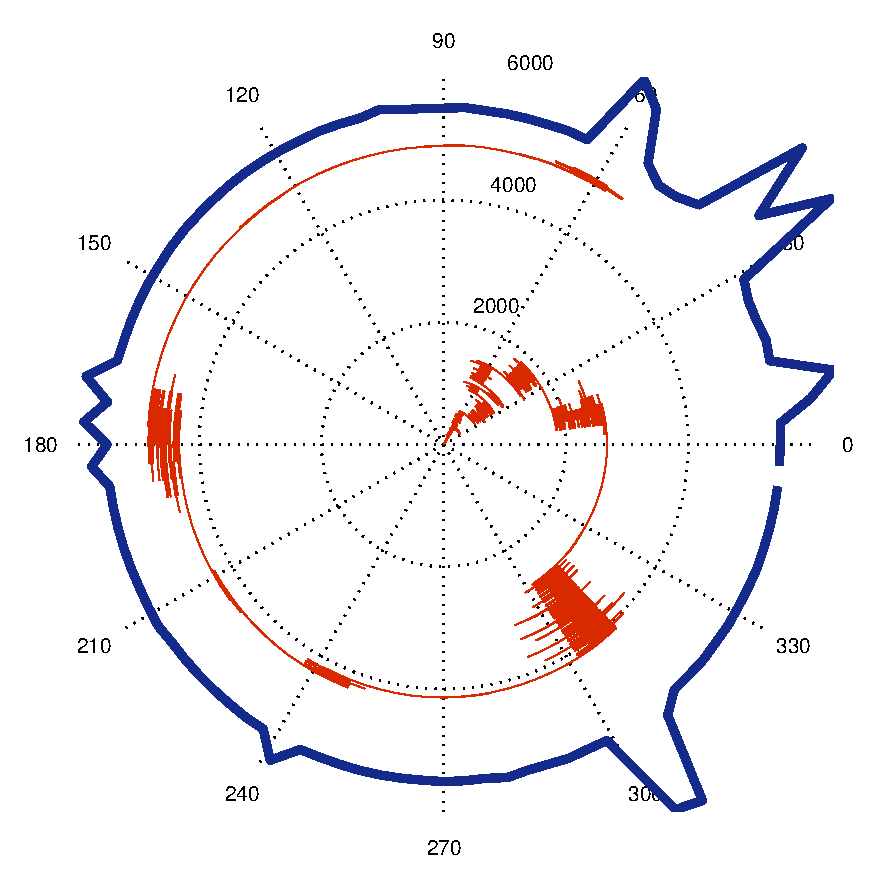
\includegraphics[height=6.5cm]{/Figs/polar_1_a.eps}
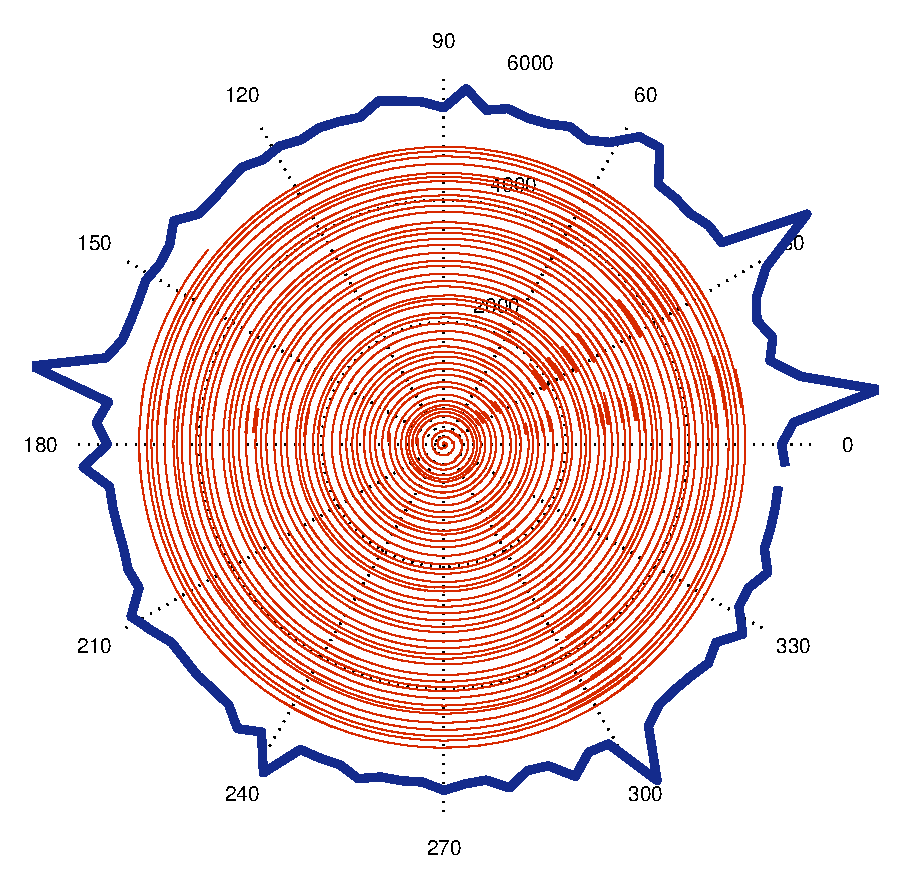
\includegraphics[height=6.5cm]{/Figs/polar_2_a.eps}
\caption{
Simulated trajectory of a particle on a disordered ring. The radial direction is time and the angle is the position. 
For small $s$ (top panel) the dynamics is overdamped, while for large $s$ (bottom panel) the dynamics is under damped. 
The thick line on the edge of the circle is the steady state distribution (See \Ap{Ap12}). For this figure there are $N=100$ sites, $\sigma=5$ and $s=0.88, \ 2.97$.
%Each panel shows several trajectories with the particle at randomly selected initial positions.
}
\label{traj}
\end{figure}

%%%%%%%%%%%%%%%%%%%%%%%%%%
%\begin{figure}[h]
%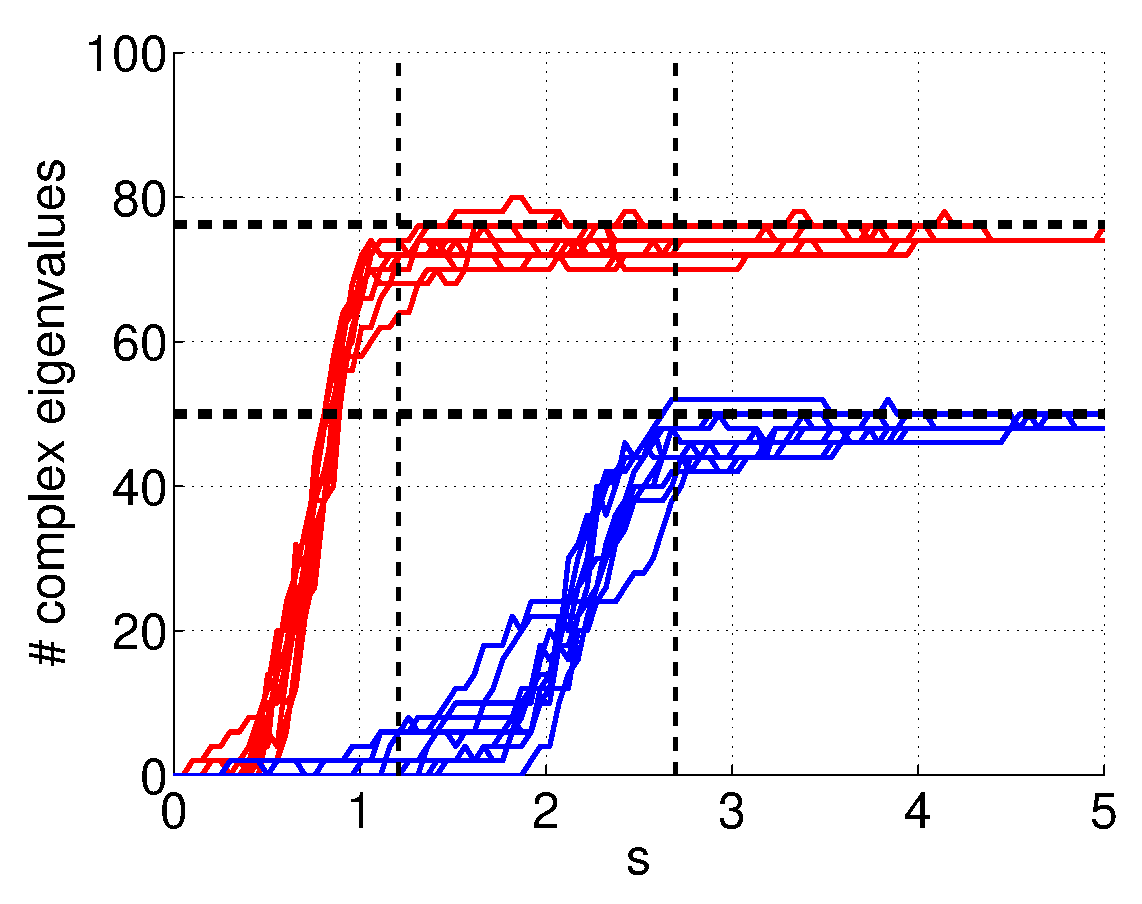
\includegraphics[height=5cm]{/Figs/numComplex_100}
%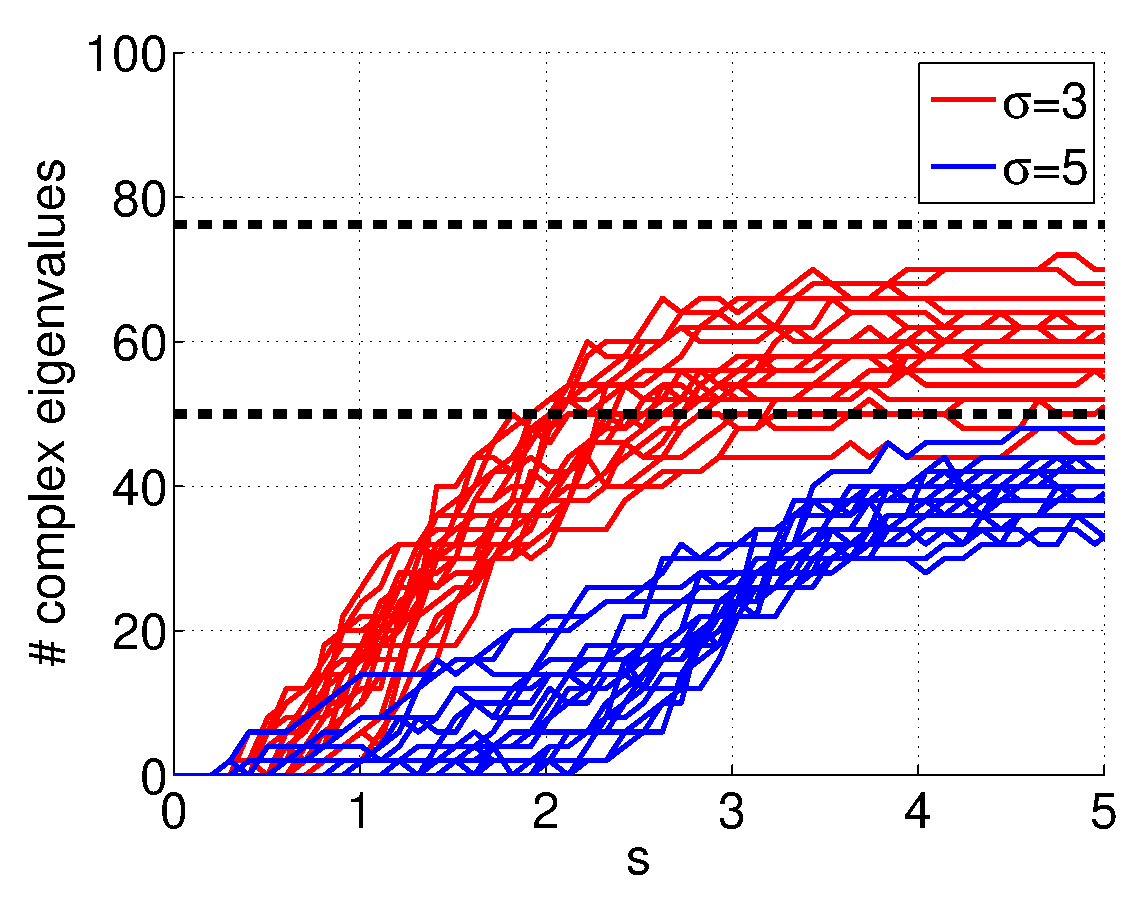
\includegraphics[height=5cm]{/Figs/numComplex_100_alpha}
%%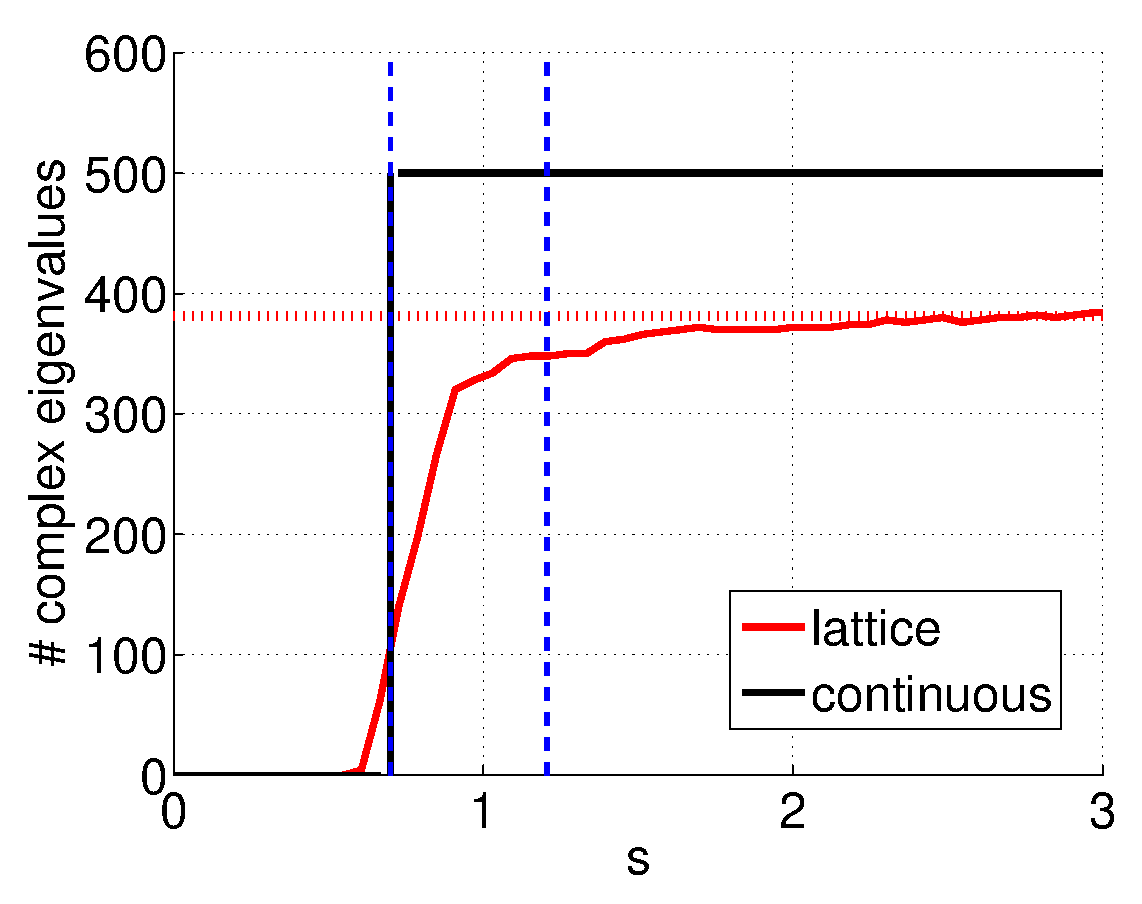
\includegraphics[height=5cm]{/Figs/numComplex_500}
%\caption{
%We count the number of complex eigenvalues
%for a ring with $N=100$ sites, for various values of the affinity $s$. Each red line corresponds to a different
%realization of field disorder with $\sigma=3$ (red) and $\sigma = 5$ (blue). 
%The black vertical lines are at values of $s_1(\sigma)$
%at which the sliding transition occurs. We see that the asymptotic fraction of complex eigenvalues saturates,
%which is quite different from what is known for non-conservative non-Hermitian matrices. The horizontal
%dashed line are analytical estimates of \Eq{e101}. 
%If the lattice were continuous and the disorder white noise, the number of complex eigenvalues would 
%go from 0 to 100 at $s=s_{1/2}$.
%On the bottom panel $\alpha=0.9$, the crossover is blurred and the saturation value is lower (the horizontal lines are calculated for $\alpha=\infty$).
%}
%%Top: Number of complex eigenvalues vs. $s$ for $N=100$ sites. 
%%Each red line corresponds to a different 
%%realisation of field disorder with $\sigma=3$ (red) and $\sigma=5$ (blue), and $\alpha=\infty$. The black vertical lines are at values of $s_1(\sigma)$ at which the sliding transition occurs.
%%Bottom: Number of complex eigenvalues vs. $s$ for $N=500$ sites and $\sigma=5$ (red)
%%vs. the result of the continuous, white noise, problem (black step function). 
%%The vertical dashed lines are $s_{1/2}$ and $s_1$. The dotted horizontal red line is the estimated saturation value, \Eq{e101}. 
%\label{figCplxSat}
%\end{figure}

%%%%%%%%%%%%%%%%%%%%%%%%%%%%%%%%%%%%%%%%%%%%%%%%%%%%%%%%%%%%%%%%%%%%%%%%%%%%%%%%%%%%%%%%%%%%%%%%%%%%%%%%%%%%%%%%%%%%
\section{Scope}

Our objective is to understand how the spectral properties of
the $\bm{W}$ matrix are affected as the affinity~$s$ is increased. 
A crucial observation is that the conservative property of 
the matrix implies that~$s$ affects not only the stochastic field, 
but also the diagonal elements. As in the work of \cite{Shnerb1} 
we can transform $\bm{W}$ into a non-hermitian $\bm{H}$ matrix.
This matrix features the following properties: 
{\ \bf (i)}~Off-diagonal disorder characterized by~$\alpha$;  
{\ \bf (ii)}~An affinity parameter~$s$. 
{\ \bf (iii)}~Diagonal disorder that is implied by the conservativity.
%
It is the last property that implies a dramatically different 
spectral scenario. In particular we would like to address the 
following questions:    
%
{\ \bf (1)}~How does the relaxation rate of the system depend on~$s$?
{\ \bf (2)}~What determines the threshold $s_c$ for getting a complex quasi-continuum?
{\ \bf (3)}~Why is there, and what determines the saturation of complexity?
{\ \bf (4)}~How is the sliding transition reflected in the spectrum?
{\ \bf (5)}~How is the percolation transition reflected in the spectrum?

In order to answer the above questions we translate the spectral problem 
into the language of Electrostatics in the two dimensional complex plane. 
%
Within the electrostatic picture we consider a system with charge density 
given by \Eq{e3} and derive a general criterion for the spectrum to become complex.
We show how the sliding transition 
thresholds $s_{\mu}$ are expressed in the spectral properties. 
In particular we show that ${s_c \rightarrow s_{1/2}}$, 
is the field required to get a sliding transition for~$D$.
We then apply the same criterion to several cases of interest.
%
{\ \bf (a)} We first explain that for a system with a wide distribution of symmetric transition rates ($\alpha < \infty, \sigma = 0$),
the delocalization process is determined 
by the percolation transition. 
We argue that for $\alpha<1/2$ the system is localized for any $s$ 
and that for $\alpha>1/2$ the system becomes delocalized for any $s>0$.
%
{\ \bf (b)} We address the simplest problem of a clean $N$-site ring with sparse field disorder.
We explain that \rmrk{$s_c \sim \sigma \sqrt{M}/N$}, 
which is the field required to overcome $M$ field defects.
%
{\bf {(c)}} We address the problem of a uniform stochastic field with a weak link, 
such that one of the $\bar{w}_n$'s is smaller than the rest. 
%
%{\ \bf (d)} Then we discuss a fully disordered ring. We show how the sliding transition 
%thresholds $s_{\mu}$ are expressed in the spectral properties. 
%In particular we show that ${s_c \rightarrow s_{1/2}}$, 
%which is the field required to get a sliding transition for~$D$.
%
{\ \bf (d)} Returning to the case of a fully disordered ring, we realize that for $s>s_{\infty}$, the real spectrum of an open chain is gapped. 
But for a closed ring the delocalization transition leads 
to a non-gapped complex $\lambda$-spectrum, that exhibits complexity saturation. 
%
{\ \bf (e)} We explain how the percolation-related transition affects the delocalization process.  
We show that for $\alpha < 1$ the saturation value is lower and that the crossover region is wider.
%



%%%%%%%%%%%%%%%%%%%%%%%%%%%%%%%%%%%%%%%%%%%%%%%%%%%%%%%%%%%%%%%%%
\section{Outline}

\begin{itemize}

%\item
%Diffusion and relaxation ($\lambda_1$ vs $s$)

\item
The secular equation for $\lambda_k$.

\item
The real spectrum  $\epsilon_k$ (discussing $\mu_s$ and $\mu_{\alpha}$). 

\item
The complex spectrum - Electrostatics.

\item
Determination of $s_c$. 

\item 
Complexity diminishes the real gap.

\item
Complexity saturation for $s \gg s_{\infty}$. 

\end{itemize}


Supplementary

\begin{itemize}

\item
Sliding transition - the definition of $s_{\mu}$.

\item
The similarity transformation (definition of $H$).

\item
The formula for the spectral determinant.

\item
Clean ring. 

\item
Ring with weak link ("$g$").

\item
Ring with single field defect.


\item
Ring with white disorder ("French").

\item
Step by step electrostatics. 

\end{itemize}



%%%%%%%%%%%%%%%%%%%%%%%%%%%%%%%%%%%%%%%%%%%%%%%%%%%%%%%%%%%%%%%%%%%%%%%%%%%%%%%%%%%%%%%%%%%%%%%%%%%%%%%%%%%%%%%%%%%%
\section{The secular equation}

Consider a stochastic process on an ${N}$-site ring with lattice spacing $a=1$, 
that is generated by a rate equation with near-neighbor hopping 
as described by the matrix $\bm{W}$ of \Eq{e2}, 
where the site index $n$ is defined modulo~$N$. 
For convenience we use the following notations:
%
\beq
\ora{w}_n &=& w_{n+1,n} \ = \ w_n \ \eexp{+\mathcal{E}_n/2} \\
\ola{w}_n &=& w_{n,n+1} \ = \ w_n \ \eexp{-\mathcal{E}_n/2}
\eeq
%
%The eigenvalues of the $\bm{W}$ matrix are denoted${\{ -\lambda_k \}}$. 
%Due to the conservativity of $\bm{W}$, the non-equilibrium steady state (NESS) is associated with ${\lambda_0=0}$. 
%The remaining eigenvalues have negative real part, 
%corresponding to decay modes and may be complex.
%The complexity of the other eigenvalues implies 
%that the relaxation process in not over-damped. 
%
% %
The question arises whether the sliding transition affects  
the global properties of the spectrum. In order to address 
this question we have to analyze the secular equation that 
is associated with the matrix~$\bm{W}$. 
%%%%%%%%%%%%%%%%%%%%%%%%%%%%%%%%%%%%%%%%%%%%%%%%%%%%%%%%%%%%%%%%%%%%%%%%%%%%%%%%%%%%%%%%%%%%%%%%%%%%%%%%%%%%%%%%%%%%
%\section{The secular equation}

By a similarity transformation of~ $\bm{W}$ one obtains
%
\be{16}
\tilde{\bm{W}} \ \ = \ \ \text{diagonal}\{-\gamma_{n}\} \ + \ \text{offdiagonal}\{w_{n}\eexp{\pm s/2}  \}
\eeq
%
where the "$\pm$" are for the "forward" and "backward" transitions respectively.
Note that the statistics of the $\mathcal{E}_n$ is still hiding in the diagonal elements.
The associated symmetric matrix $\bm{H}$ is defined by setting ${s=0}$.
Then one can define a spectral determinant $S(z)$ and associated spectrum as follows:
%
\beq
 \det(z-H) \ \ = \ \ \prod_k (z+\epsilon_k) \ \ = \ \ S(z)
\eeq
%
If the system is an  ${N}$-periodic infinite lattice, 
then ${\bm{W}}$ is similar to ${\bm{H}}$ by "gauge" transformation, 
hence one can regard the ${\{-\epsilon_k\}}$ as the spectrum of  an open chain.
But if the system is an ${N}$-periodic ring (periodic boundary conditions) 
then $s$ cannot be "gauged" away. 
Still there is a simple relation \cite{det1} that relates 
the spectral determinant of~$\bm{W}$ to that of~$\bm{H}$. Namely, 
%
\be{17}
\det(z-W) \ = \  \prod_k (z+\lambda_k)  \ \ \equiv \ \ S(z)-S_0 
\eeq
%
where
%
\beq
S_0 \ \ = \ \ 2\left[\cosh\left(\frac{Ns}{2}\right)-1\right]  \prod_n w_n
\eeq
%
The roots ${z=-\lambda_k}$ have real negative part, but may be complex in general.
The lowest eigenvalue ${\lambda_0=0}$ corresponds to the non-decaying 
non-equilibrium steady state (NESS). It is implied that 
%
\beq
S(0)=S_0 \ \ \ \ \ \ \ \text{implication of conservativity}
\eeq
%
We emphasize that the latter property is not true for a general 
non-Hermitian matrix, neither is the "positivity" of the ${\lambda_k}$.  
This has far reaching implications: in particular it should be 
clear that the NESS is an extended state, hence it follows that 
the localization length has to diverge in the limit ${\lambda\rightarrow0}$.
This is in essence the difference between the 
conventional Anderson model (Lifshitz tails at the band floor) 
and the Debye model (phonons at the band floor).     

From the above it follows that the secular equation for the $\lambda$ 
spectrum can be written as  
%
\be{20}
\prod_k \left(\frac{z+\epsilon_k(s)}{\overline{w}}\right) \ \ = \ \ 2\left[\cosh\left(\frac{Ns}{2}\right)-1\right]
\eeq
%
where ${\overline{w}}$ is the geometric average of all the rates.
The affinity~$s$ affects both the $\epsilon_k$ and the right hand side.

%%%%%%%%%%%%%%%%%%%%%%%%%%%%%%%%%%%%%%%%%%%%%%%%%%%%%%%%%%%%%%%%%%%%%%%%%%%%%%%%%%%%%%%%%%%%%%%%%%%%%%%%%%%%%%%%%%%%
\section{The real spectrum}

The main observation regarding the real spectrum $\epsilon_k$ of the associated symmetric matrix $\bm{H}$ 
is that for $s<s_{\infty}$ it is gapless and for $s>s_{\infty}$ a gap opens up. 
This can be seen both in the spetcral density and in the electrostatic potential along the real axis. Recall that  $\rho(\epsilon)\sim \epsilon^{\mu-1}$.
Consider first the case $\alpha \gg 1$, the percolation aspect is absent and $\mu=\mu_s$.
The simplest case is for $s>s_{\infty}$, where a gap opens up at $\epsilon_0 = e^{(s-\sigma)/2}$ and the spectral density is distributed log-box,
$\rho(\epsilon) = {N}/{\sigma \epsilon} $.
This holds as long as   $\alpha\gg 1$. The interesting case 
is when  $\alpha \lesssim 1$ and $s<s_{\infty}$, 
now there is a crossover in the spectrum between two anomalous behaviours. 
The bottom of the band is detemined by~${\mu_s}$ 
and the top of the band  by  ${\mu_{\alpha}}$, as show in  \Fig{fig2}.
As $\alpha$ decreases, the $\mu_s$  determined region becomes smaller.
%
This crossover is analogous to regular diffusion, where there  is a crossover from short time, diffusion limited spreading to long time drift limited spreading. 
In our case the crossover is from low energy (long time) sliding ($\mu_s$) to high energy (short time) percolation limited diffusion $\mu_{\alpha}$.
%

We remark that the the case of a continuous and open system with 
stochastic field that is guassian white noise has been studied extensively in \cite{odh3}.
Exact analytical results for the density of states and inverse localization (electrostatic potential) 
length were obtained (these are summarized in \Ap{A9}). 
We emphasize that the results of \cite{odh3} do not account for bond disorder and thus do not supply additional information (as shown in \Fig{fig2}), since it would be relevant only in the small $\epsilon$ regime in which the density of states calculated in \cite{odh3} reduces to that of \Eq{e7}.
It is noteworthy that, the electrostatic potential in \cite{odh3}
has a peculiar trait that  $V(\epsilon \to \infty) = \text{const}$,  
implying that the entire spectrum goes from real to complex at $s=s_{1/2}$, 
which is quite different than the complexity saturation effect in our model. 

%
\begin{figure}
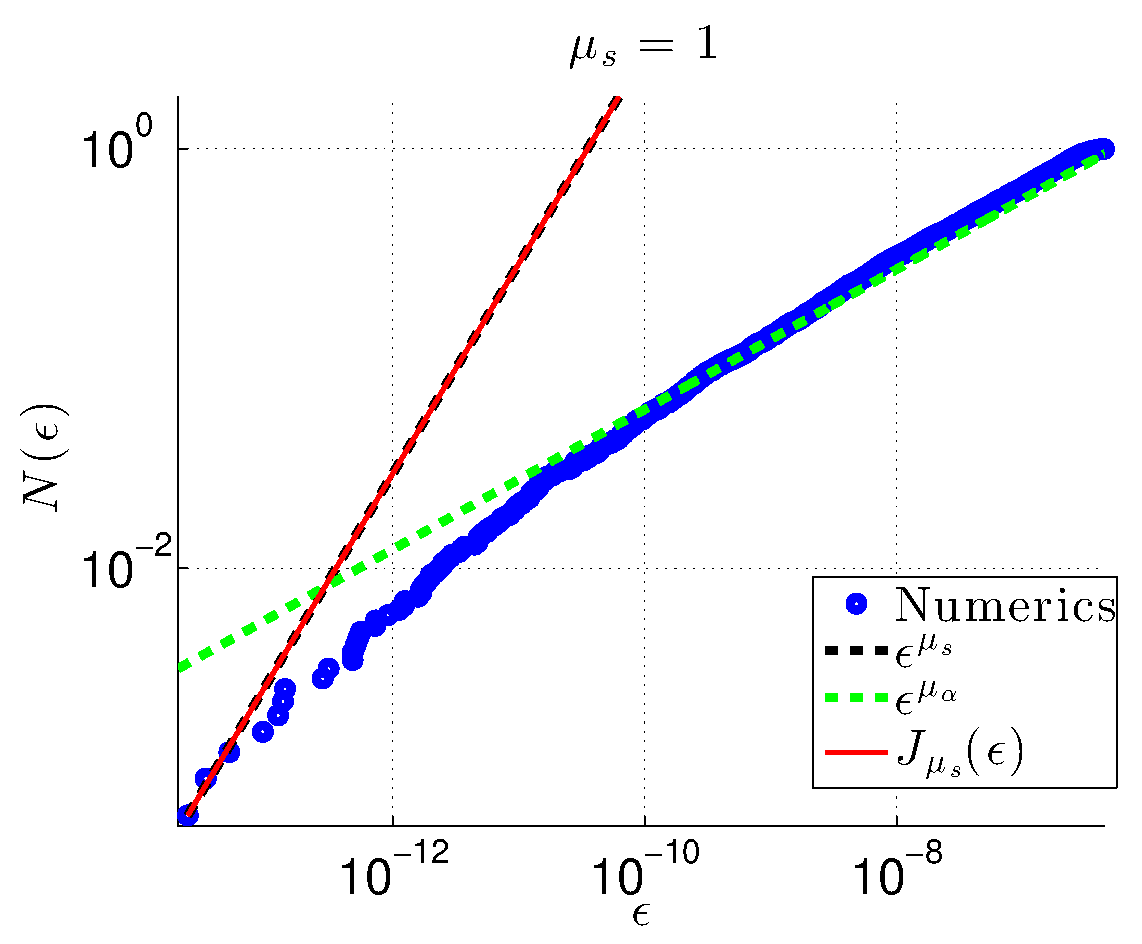
\includegraphics[height=5cm]{/Figs/N_E_1_1_french}
\caption{The integrated density of the $\epsilon_k$ for a ring with ${N=5000}$ sites. The
system is characterized by a percolation exponent ${\mu_{\alpha} = 1/3}$ and a scaled affinity ${\mu_s = 1}$.
 The width of the stochastic-field distribution is $\sigma=2$. 
 The blue points are are results of numerical diagonalization. 
 There is a crossover from density that corresponds to $\mu_s$ (dashed black line) to density that corresponds to $\mu_{\alpha}$ (dashed
green line). The thin red line is the result of \cite{odh3}, for small $\epsilon$, it coincides with the power law behavior that we assumed.
}
\label{fig2}
\end{figure}

%%%%%%%%%%%%%%%%%%%%%%%%%%%%%%%%%%%%%%%%%%%%%%%%%%%%%%%
%%%%%%%%%%%%%%%%%%%%%%%%%%%%%%%%%%%%%%%%%%%%%%%%%%%%%%%%%%%%%
\section{Electrostatics}

In order to get an insight into the secular equation we 
define an "electrostatic" potential as follows:
%
\be{22}
\Psi(z) \ \ = \ \ \sum_k \ln\left(\frac{z-\epsilon_k}{\overline{w}}\right) \ \ \equiv \ \ V(x,y)+iA(x,y)
\eeq
%
where ${z=x+iy}$.
 Note that compared with \Eq{e16} 
we have flipped the sign convention (${z\mapsto -z}$).
The potential for a given charge distribution $\rho(x)$ is 
%
\be{21}
{V(x,y)=\frac{1}{2} \int \ln \left[(x-x')^2 + y^2\right] \rho(x')dx'} 
\eeq
%
and along the real axis it is
%
\be{23}
V(\epsilon) =  \int \ln \left(|\epsilon-x \right|) \rho(x)dx 
\eeq
%
The constant ${V(x,y)}$ curves correspond to potential contours,
along which $|S(z)|$ is constant, and the constant ${A(x,y)}$ curves corresponds 
to stream lines, along which the phase of $S(z)$ is constant. 
The derivative $\Psi'(z)$ corresponds to the field, which can be regarded as 
either electric or magnetic field up to a 90deg rotation.       
Using this language the secular equation takes the form
%
\beq
V(x,y)=V(0); \ \ \ \ A(x,y)=2\pi*\text{integer} 
\eeq
%
Namely the roots are the intersection of the field lines with the 
potential contour that goes through the origin. 

\clearpage
\onecolumngrid

\begin{figure}
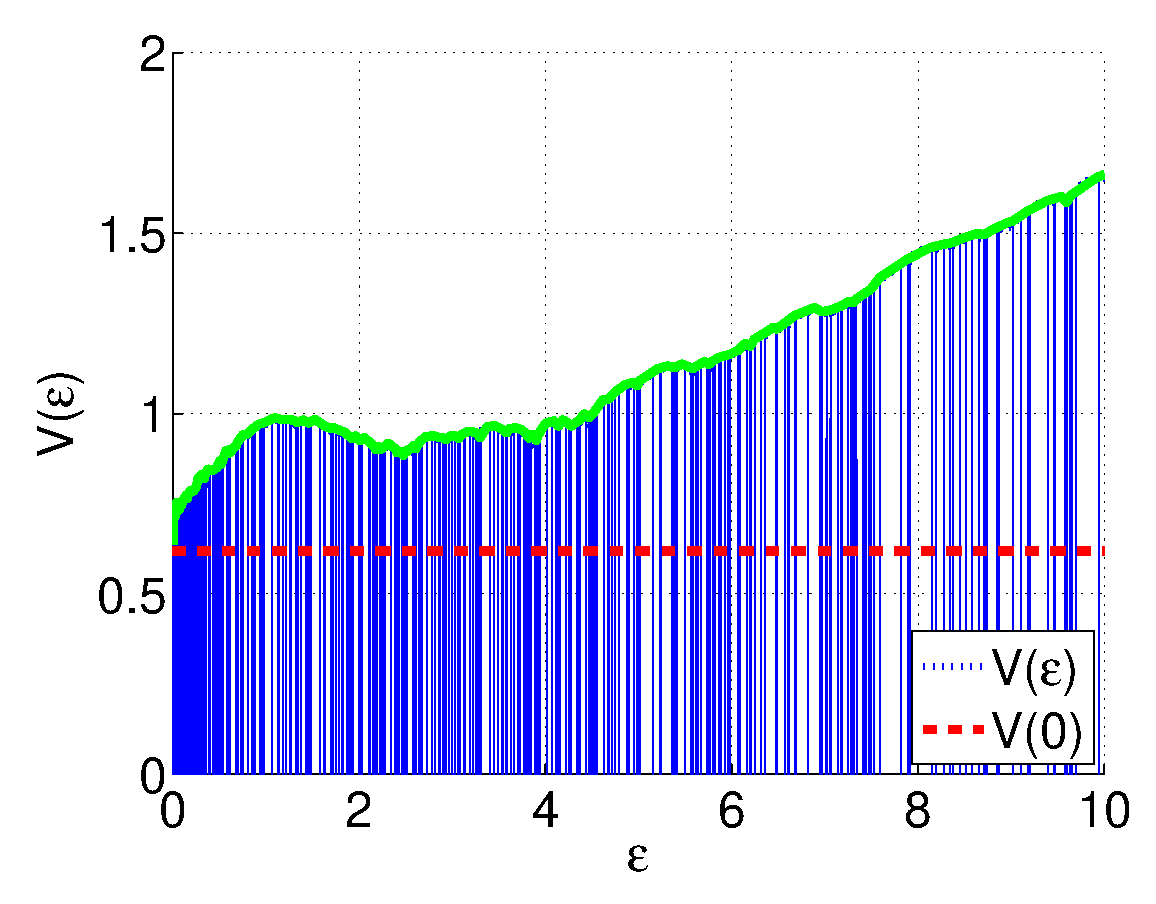
\includegraphics[height=4.5cm]{/Figs/V_E_1_2.eps}
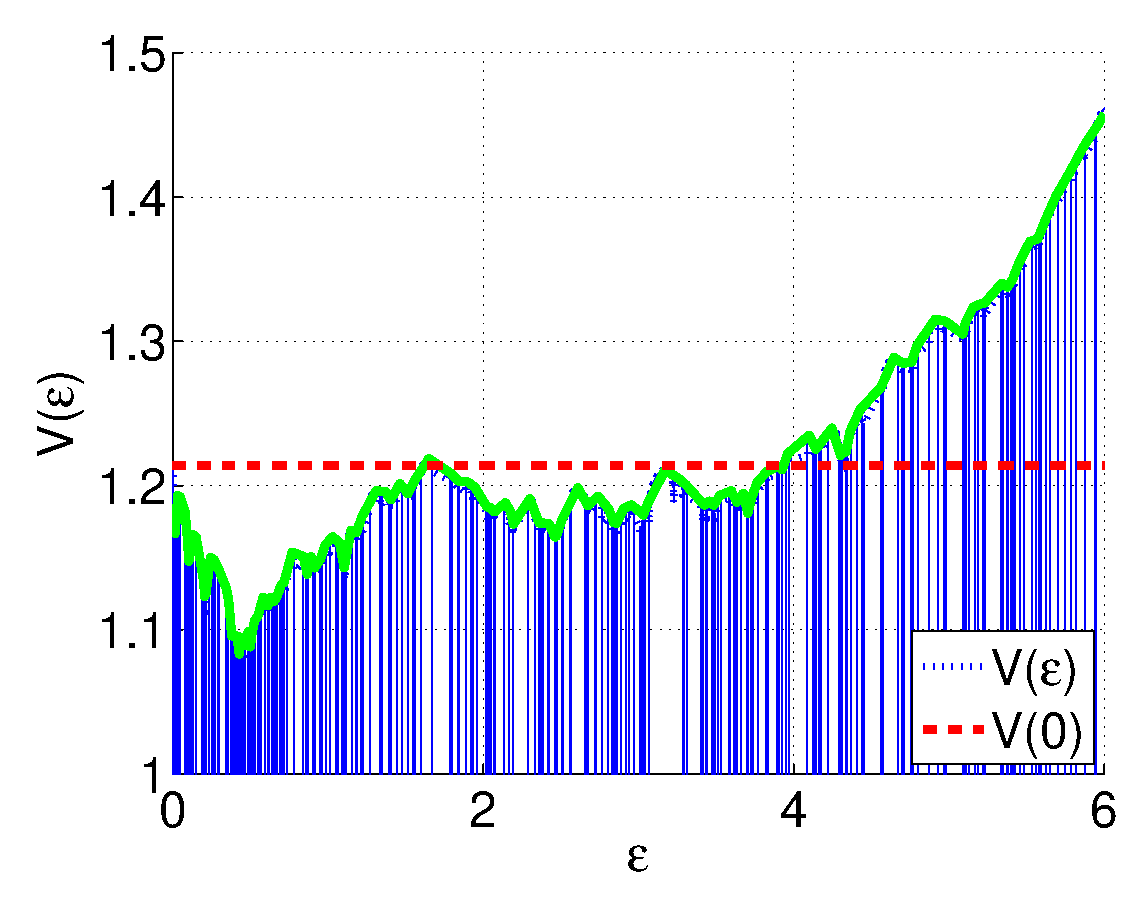
\includegraphics[height=4.5cm]{/Figs/V_E_1.eps}
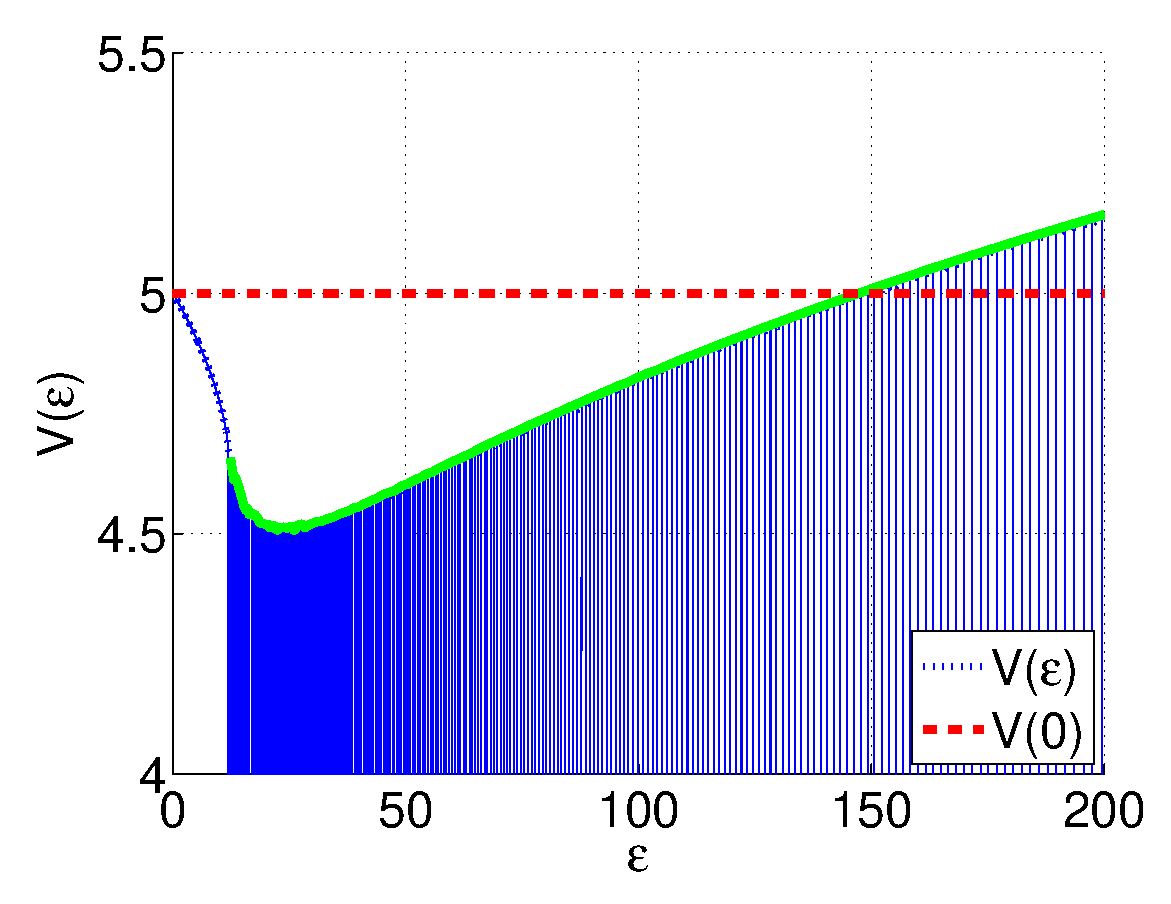
\includegraphics[height=4.5cm]{/Figs/V_E_2.eps}

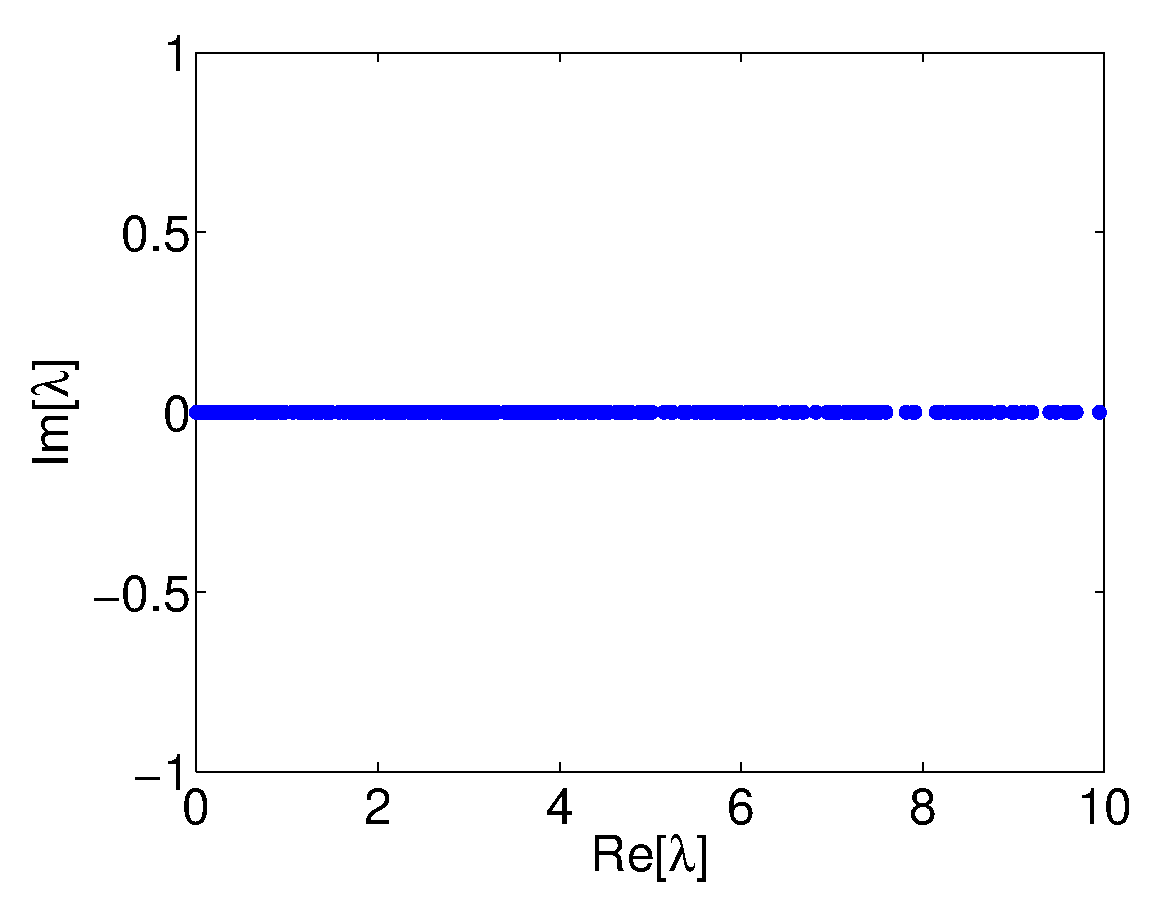
\includegraphics[height=4.5cm]{/Figs/spectrum_1_2.eps}
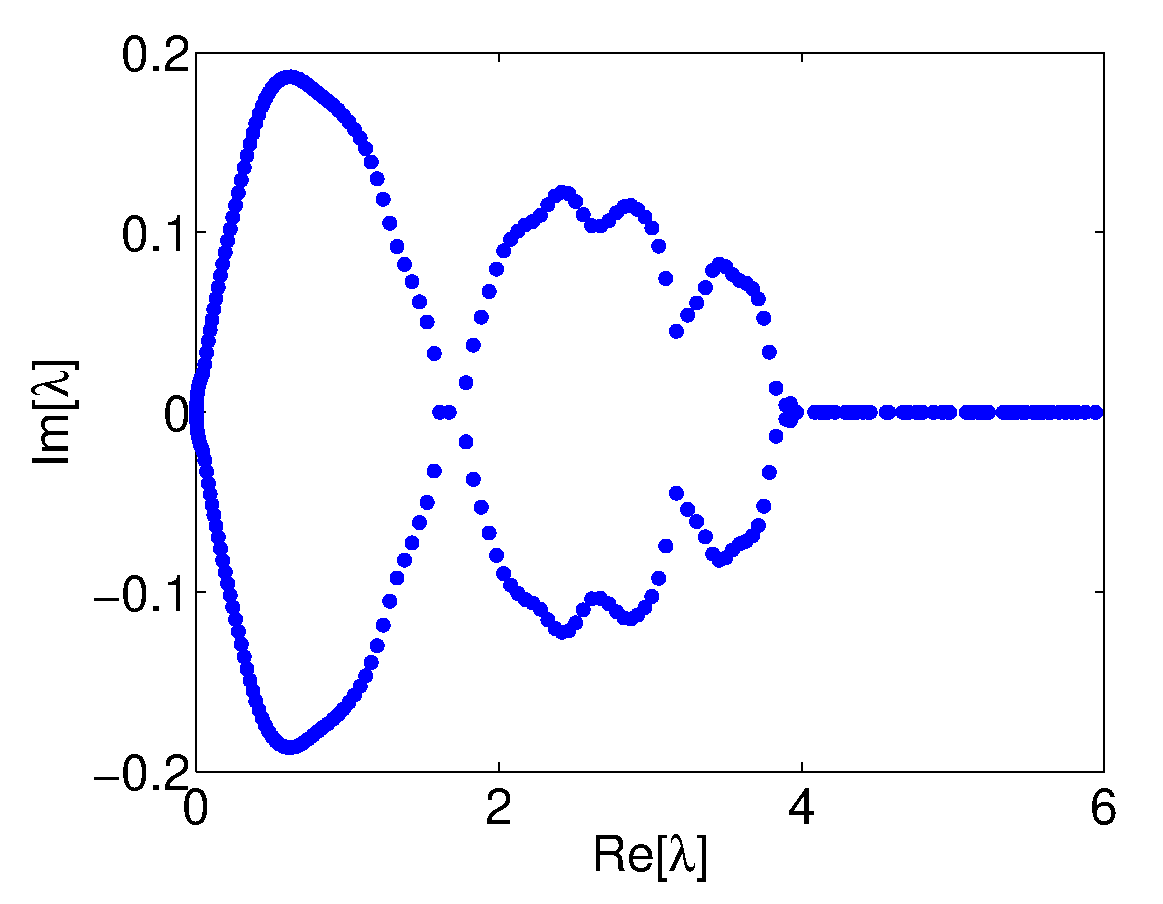
\includegraphics[height=4.5cm]{/Figs/spectrum_1.eps}
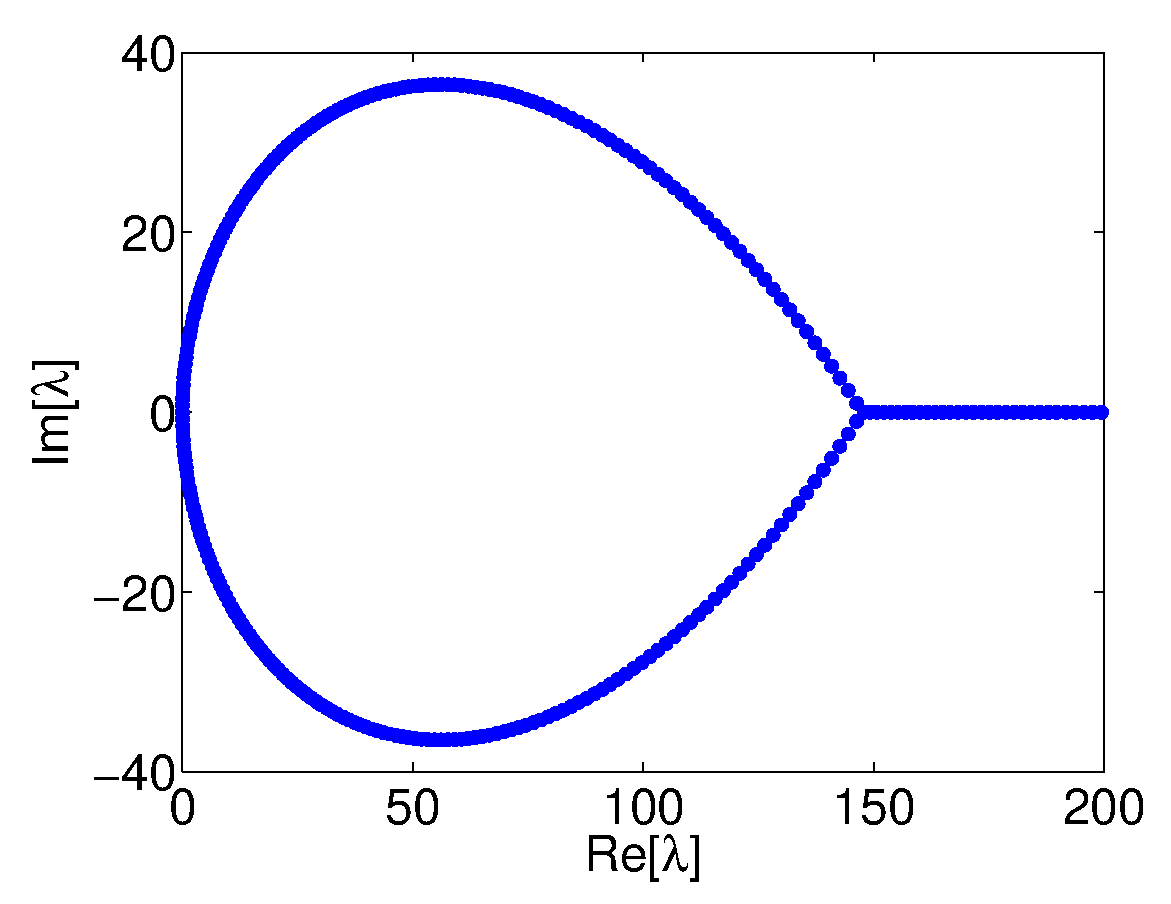
\includegraphics[height=4.5cm]{/Figs/spectrum_2.eps}
\caption{
Illustrating the route to complexity. The top row shows 
the electrostatic potential $V(\epsilon)$ along the real axis and the bottom row shows the associated spectrum in the complex plane. 
Here $N=500$, $\sigma = 5$, and (from left to right) $s=1.24, \ 2.43,\ 10$. For these parameters the threshold values are $s_{1/2}=1.77, \ s_1=2.7$ and $s_{\infty}=5$.
In the left hand column $s<s_{1/2}$ and the spectrum is real.
In the middle column $s_{1/2} <s <s_{\infty}$ and there is an interesting scenario of a mixed spectrum, where there might be several complex bubbles separated by real segments. 
In the right hand column  $s>s_{\infty}$ and the real spectrum has a gap (beginning with the first oscillation), but the complex spectrum does not (see also \Fig{figWeak}). 
Also, the spectrum is a fully developed complex bubble, where the bottom of the band is delocalized (underdamped modes) and the rest of the band 
is localized (or overdamped).
}
\label{f2}
\end{figure}

\twocolumngrid

%%%%%%%%%%%%%%%%%%%%%%%%%%%%%%%%%%%%%%%%
\section{Determination of $s_c$}

From the preceding section
we know that the potential at the origin is 
%
\beq
V(0) \ \ = \ \ \ln\left[2\cosh\left(\frac{Ns}{2}\right)-2\right]
\eeq
%
From a straightforward electrostatic calculation we find 
that for a charge density that is given by \Eq{e3} with some cutoff $\epsilon_c$,
the derivative of the electrostatic potential at the origin is 
given by (see \Ap{A1} for derivation)
%

\be{19}
V'(\epsilon) \approx  \frac{ \epsilon^{\mu-1}}{\epsilon_c^{\mu}} \pi \mu \cot(\pi \mu)
%V'(0) \sim \mu \cot(\pi \mu)
\eeq

%
Indicating that the sign changes from positive to negative at $\mu=1/2$.

Let us make a few observations regarding the potential $V(\epsilon)$ along the real axis.
For an illustration see \Fig{f2}. Clearly if the envelope of $V(\epsilon)$ is above 
the $V=V(0)$ line, then the spectrum is real, and the $\lambda_k$ are roughly 
the same as the $\epsilon_k$, shifted a bit to the left. 
The second observation is that the envelope of $V(\epsilon)$ is positive 
in segments where the $\epsilon_k$ forms a quasi-continuum. 
This follows from the observation that $(1/N)V(\epsilon)$ equals 
the inverse localization length \cite{Shnerb1}.
% 
In the case under study the quasi-continuum starts at ${\epsilon_s=0}$ 
for ${s<s_{\infty}}$ (\Fig{f2}), and at finite ${\epsilon_s}$ for ${s>s_{\infty}}$ (\Fig{figWeak}).
If follows that the threshold $s_c$ f,or getting a complex quasi-continuum 
is either ${V'(0)<0}$ or ${V(\epsilon_s)<V(0)}$ respectively. 
In the former case it follows from \Eq{e19} that ${s_c=s_{1/2}}$.
%
%\begin{figure}
%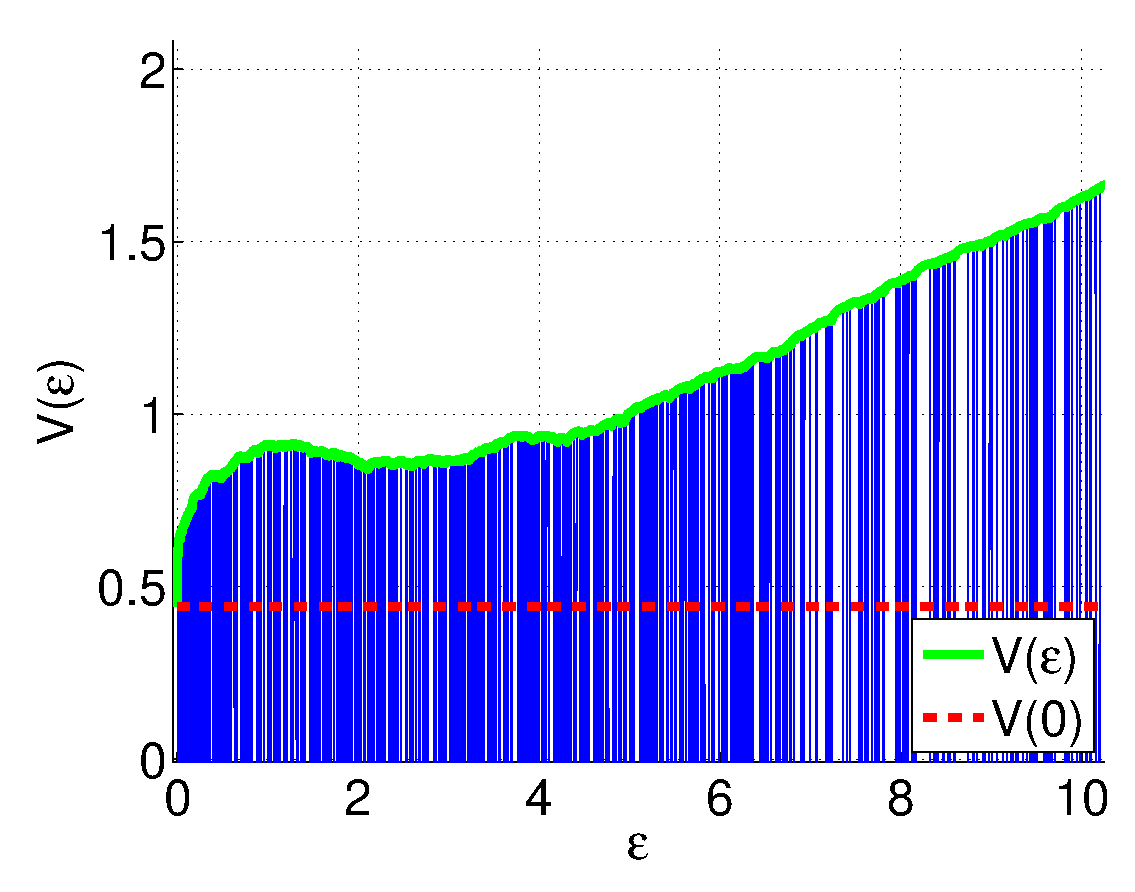
\includegraphics[height=5cm]{/Figs/V_E_localized.eps}
%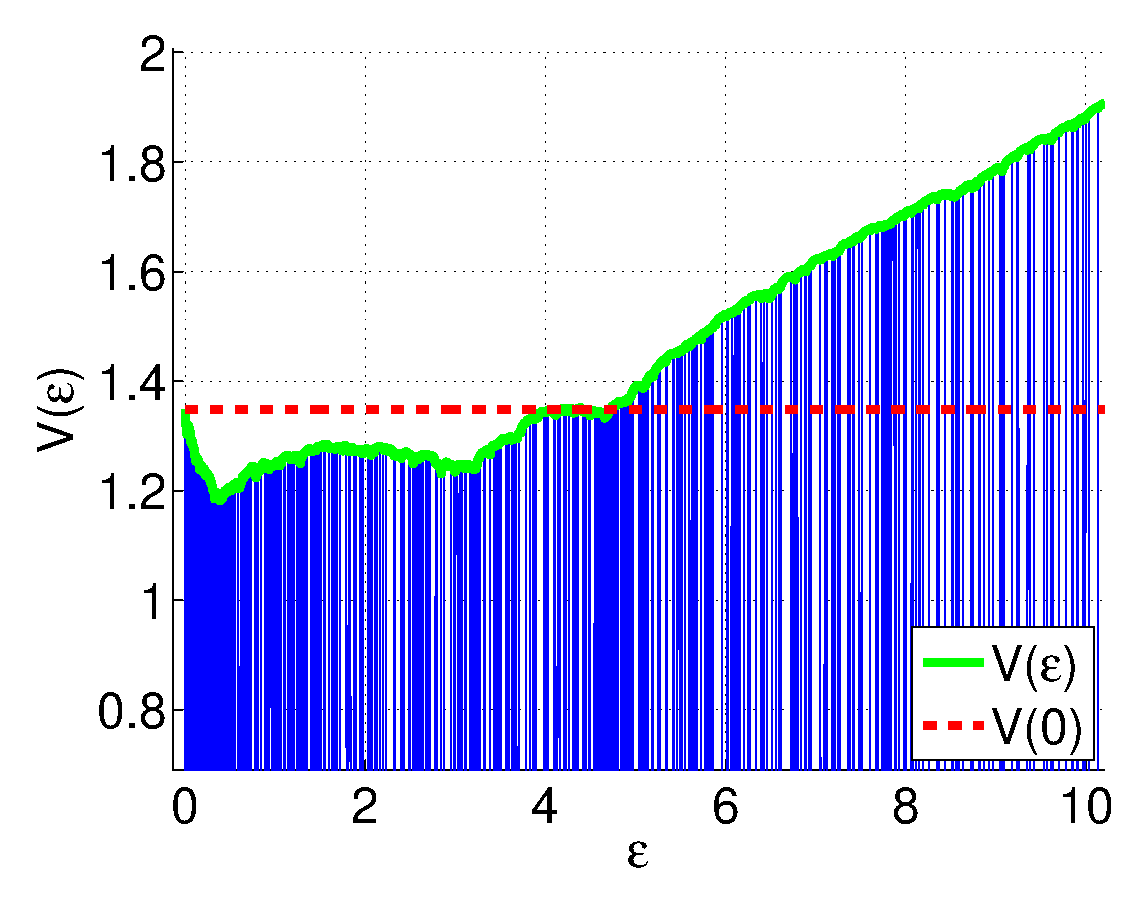
\includegraphics[height=5cm]{/Figs/V_E_delocalized.eps}
%\caption{
%The electrostatic potential $V(\epsilon)$ along the real axis. Here $N=1000$, $\sigma = 5$. 
%On the top panel $s<s_{1/2}$ and the spectrum is real.
%On the bottom panel $s>s_{1/2}$ and the spectrum becomes complex complex. 
%For $s > s_{\infty}$ the real spectrum has a gap as illustrated in \Fig{figWeak}a.}
%\label{f}
%\end{figure}
%%
%
%
%%%%%%%%%%%%%%%%%%%%%%%%%%%%%%%%%%%%%%%%%%%%%%%%%%%%%%%%%%%%%%%%%
%
\subsection{Determination of $s_c$ - Random resistor network with uniform field} 
\label{s8_1}
%
We consider now the case where all of the bonds are random and the field is uniform, $s\neq  0, \ \sigma=0$.
Using the electrostatic picture we have shown that $\mu=1/2$ provides the threshold value for complex eigenvalues. 
All one has to do is determine what is $\mu$ for the problem at hand. 
Recall that $\mu$ is the exponent of the associated real spectrum of ${\bm H}$.
For $s=0$, we already know $\mu$ is given by \Eq{e5}.
For large $s$, the matrix ${\bm H}$ is characterized by very large diagonal elements, ${\gamma_k = w_{k} e^{s/2} \gg w_k}$
and is thus "trivially localized" with eigenvalues $\epsilon_k = \gamma_k$. 
Therefore $\mu(s\gg 1) = \alpha$, by definition of $w_k$ (\Eq{e4}), 
while for small $s$, the exponent is given by \Eq{e5}.
So, for ${\alpha<1/2}$ also $\mu<1/2$ and the electrostatic picture tells us that the spectrum must be real, regardless of $s$.
On the other hand, if $\alpha>1/2$ also $\mu>1/2$ and the spectrum will become complex for any finite $s>0$.
%%%%%%%%%%%%%%%%%%%%%%%%%%%%%%%%%%%%%%%%%%%%%%%%%%%%%%%%%%%%%%%%%


\subsection{Determination of $s_c$ - white vs. sparse field disorder} 

The simplest case to exhibit a crossover to a complex spectrum is that of a single defect. 
There are two types of defects, either in the couplings $w_n$ or in the fields $\mathcal{E}_n$. 
The details are slightly different, but the analysis is essentially the same. 
The spectrum $\epsilon_k$ of the symmetric matrix $\bm{H}$ has two components: 
A continuum in the range $2\cosh(s/2)\pm 2$ and two additional states.
There are two additional states because by changing a single bond, two decay rates are altered. 
In the language of electrostatics we have a continuous charge distribution and two point charges 
$\gamma_1,\gamma_2$.
In general, one of these charges is immersed in the continuum and one of the charges is isolated, either well above or well below the continuum. 
Since the continuum does not contribute to the potential $V(\epsilon_s)$ (see \Ap{A10}), 
in the end 
%
\beq
V(\epsilon_s) &=&V(|\gamma_i - \epsilon_s|)
\eeq
%
where $V(|\gamma_i - \epsilon_s|) \approx \ln\gamma_i$ 
is the potential at $\epsilon_s$, generated by a single charge at a distance $|\gamma_i-\epsilon_s|$ from the continuum.
All that is required now it to find the $\gamma_i$'s for the configuration at hand.

For a single defect in the stochastic field the decay rates are 
%
\beq
\gamma_0  &=& 2\cosh(s/2)\\
\gamma_1  &=& e^{(s+\sigma)/2} + e^{-s/2} \\
\gamma_2  &=& e^{-(s+\sigma)/2} + e^{s/2}
\eeq
%
where $\gamma_1$ is above the continuum and 
$\gamma_2$  is immersed in the continuum, 
thus $V(\epsilon_s) = \ln\gamma_1 \approx \sigma/2$, so from the condition that $V(\epsilon_s)=V(0)$ 
we get 
%
\be{32} 
s_c = \frac{\sigma}{N}
\eeq 
%
Note that this result can be obtained in the continuum limit (see Appendix).

%
This argument can be extended to the case of $M$ defects, under the assumptions that
the field strength of each defect is different and that the defects are well separated. 
If there are $M$ field defects of varying strength $\sigma_i \in [-\sigma, \sigma]$ then there are
$M$ isolated charges $\gamma_i \approx e^{\sigma_i/2}$, so the potential is 
%
\beq
V(\epsilon_s) = \sum_{i=1}^M \ln \gamma_i  = \frac{1}{2}\sum_{i=1}^M \sigma_i \sim \frac{\sigma\sqrt{M}}{2}
\eeq
From  the condition ${V(\epsilon_s)=V(0)}$, one gets the threshold value 
%
\be{33}
s_c =\frac{ \sigma}{N}\sqrt{M}
\eeq
%
%This approximation for sparse disorder is tested in \Fig{sparse}.
Of course this approximation breaks down at some finite value 
of defect density $M/N$ since the assumption that the defects are well separated is no longer valid. 
At this point there should be a crossover to the fully disordered behaviour where ${s_c \rightarrow s_{1/2}}$.
In the numerics this happened at $M/N \sim 0.1$. 
This sparse disorder approximation is tested in \Fig{sparse}.

%%%%%%%%%%%%%%%%%%%%%%%
%
%Consider first a defect in the stochastic field, all of the transition rates are $e^{\pm s/2}$ except for a single bond where the rates are $e^{\pm(s-\sigma)/2}$. As a result there are 4 different decay rates 
%%
%\beq
%\gamma_0 &=& 2e^{-\sigma/2} \cosh(s/2),\\
%\gamma_1 &=& 2\cosh(s/2)\\
%\gamma_2 &=&e^{s/2}+e^{-(s-\sigma)/2}\\
%\gamma_3 &=&e^{(s+\sigma)/2}+e^{-s/2} 
%\eeq
%%
%The spectrum $\epsilon_k$ of the symmetric matrix $\bm{H$} is 
%composed of a continuum in the range $2\cosh(s/2)\pm 2$ 
%with three additional states: $\gamma_0$, which is immersed in the contiuum while $\gamma_2, \gamma_3$ are above the continuum by a factor of $\exp(\sigma/2)$.
%%
%The continuum contributes zero to the potential at $\epsilon_s$.
%The charges above the continuum contribute ${V(\epsilon_s) = \ln\gamma_2 + \ln \gamma_3 \approx \sigma}$. From  the requirement ${V(\epsilon_s)<V(0)}$, one gets 
%%
%\beq
%s_c = \frac{2\sigma}{N} 
%\eeq
%
%%%%%%%%%%%%%%%%%%%%%%%%%%%%%%%%%%%%%%
\begin{figure}
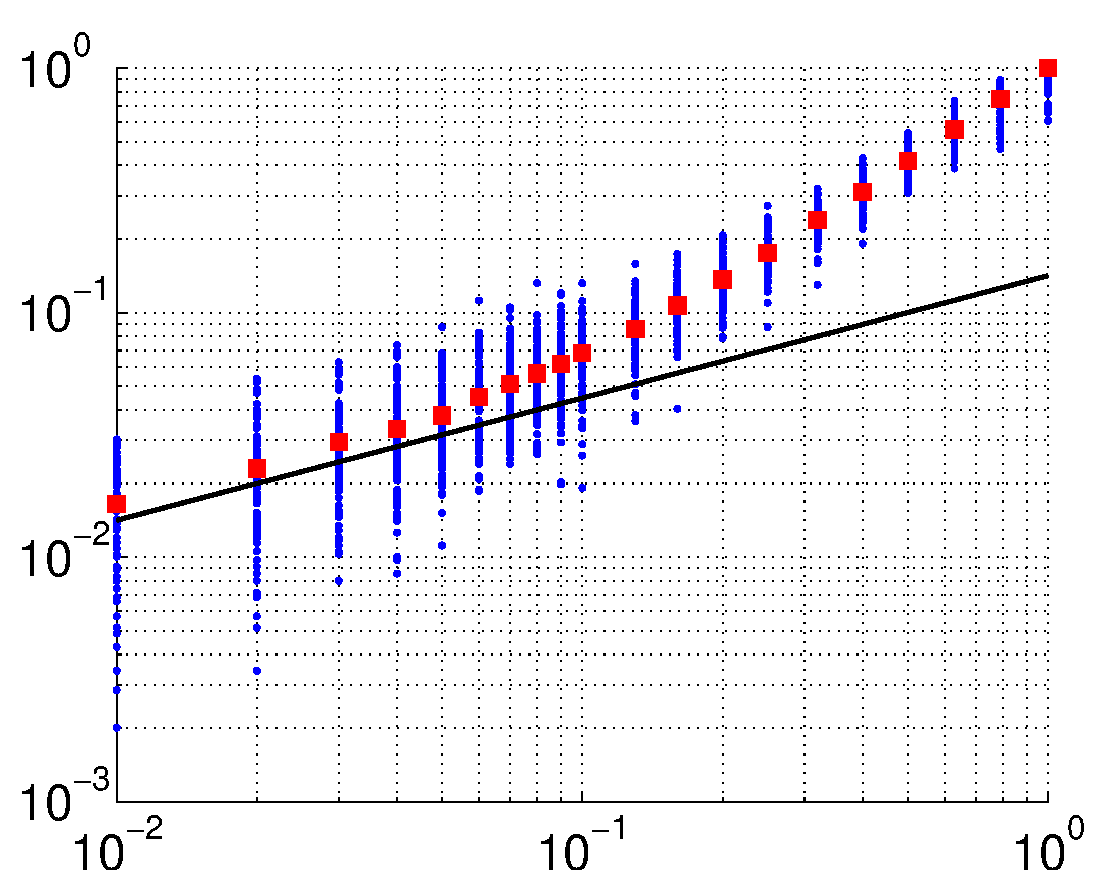
\includegraphics[height=5cm]{/Figs/s_c_sparse_100_loglog.eps}
\caption{The threshold value $s_c$ for the spectrum to be complex vs. the number of stochastic field defects $M$. Here $N=100$ sites and $\sigma=5$. 
The $x$ axis is the fraction of the lattice that has a disordered field, the rest of the lattice has a uniform field. For a fully disordered lattice we expect $s_c=s_{1/2}$, hence the scaling of the $y$ axis. 
The black line is the sparse disorder approximation, \Eq{e33}.
Blue dots correspond to 100 different realizations of disorder per $M/N$, red dots are their averages. }
\label{sparse}
\end{figure}
%%%%%%%%%%%%%%%%%%%%%%%%%%%%%%%%%%%%%%

\subsection{Determination of $s_c$ - weak link}

Consider now a single defect in the couplings, such that  $w_1 = g, \ w_{n\neq1}=1$ where $g\ll1$.
This setup can be treated exactly in the continuum limit, 
yet we can use the electrostatic picture to obtain an estimate for $s_c$ in the discrete lattice. 
In the continuum limit one considers a ring of length $L$ with diffusion coefficient $D$. 
A small segment of length $a\ll L$ has 
diffusion coefficient $D_1 \ll D$ such that $G=(L/a)(D_1/D) $  is the relative strength of the weak link. 
In the lattice version we have $g=D_1/D$.
By standard transfer matrix methods one  can derive the secular equation for the complex eigenvalues (see \Ap{A6})
%
\be{50}
 \cos(k) + \frac{1}{G} \frac{k^2+(\frac{S}{2})^2}{2k}\sin(k)= \cosh \left(\frac{S}{2} \right)
\eeq
%
where $k^2= {z L^2/D - S^2/4}$ is generally complex.
The envelope of the secular equation is
%
\beq
B(z) = \sqrt{1+\frac{1}{G^2} \frac{z^2}{4z - S^2}}
\eeq
%
and is related to the electrostatic potential by ${\Psi(z) = \ln\left[2B(z)-2\right]}$.
Note that the envelope function can be viewed as a smeared version of the potential, or alternatively 
as the $L\to \infty$ limit (where the spectrum is continuuous) of the potential.
This function has a minimum at $z = S^2/2$, thus the secular equation has real solutions provided 
%
\be{51}
\sqrt{1+\left(\frac{S}{2G}\right)^2} > \cosh \left(\frac{S}{2}\right)
\eeq
%
For $S/G \gg 1$ this equation becomes approximately ${S/(2G) = e^{S/2}}$. The solution is given in terms of the Lambert $W$ function
%
\beq
S_c = -2 W(-G/2)
\eeq
%
%
%We would like to test the electrostatic picture. 
%In the electrostatic picture, we consider the problem on a lattice. 
%As a result there is a finite number of charges. 
%

To illustrate the use of the electrostatic picture, we show to what extent one can reconstruct \Eq{e51}. 
By the prescription for finding the eigenvalues of the associated hermitian matrix $\bm{H}$, 
the charges $\epsilon_k$ are found numerically as zeros of \Eq{e50} with $S=0$ on the right hand side. 
These charges can be viewed as a forming a quasi contiuum beginning at $\epsilon_s \approx \epsilon_1= S^2/4$, 
however there must be an additional charge, $\epsilon_0 \gtrsim 0$. 
The extra charge corresponds to the state which upon analytic continuation becomes the NESS, $\lambda = 0$.
For a lattice, it would be at some finite but small value, but in the continuum limit this charge appears at the origin, so $\epsilon_0=0$.
This has to do with the fact that the region $|x|<a$ in which the diffusion coefficient is small has measure zero in the continuum limit (see \Ap{A6}).
Since the continuum does not contribute to the potential at $\epsilon_s$, 
the only contribution to the potential there is due to the charge at the origin, 
thus at $\epsilon_s$ the potential is
%
\be{511}
V(\epsilon_s) \approx \ln \left[\frac{S^2}{4C}\right]
\eeq
%
where $C$ is some constant that arises due to truncation of the spectrum and may be found by fitting.
As before, the condition for complexity is 
$V(\epsilon_s) < V(0)$.
%
Thus we have that the result in the contiuum limit (\Eq{e51}) agrees with the discrete electrostatic picture \Eq{e511} when $S/G \gg 1$.
%

%
%
%The ground state is pushed down from the quasi-continuum.
% \rmrk{(From numerical experiments, I still don't have the exact physical argument.)}
%$\epsilon_s = \epsilon_1/g = s^2/4g$.
%% $\epsilon_s = v^2/4D + D\pi^2/N^2 $ and a single
%%state $\epsilon_1 \approx s^2/4g$ that is pushed down from the continuum (but not zero). 
%%To obtain $\epsilon_1$ we use the same argument as in the continuum derivation. This ground state should be $v^2/4D$,  we assume that the local diffusion coefficient is $gD$ but that the drift velocity is not affected.
%%
%The potential at $\epsilon_s$ due to the continuum is approximately zero and the potential there, 
%generated by $\epsilon_1$ is  (Assuming $s\ll1, \ N\gg 1$)
%%
%\beq
%V(\epsilon_s) = \ln \left|\frac{\epsilon_s-\epsilon_1}{g}\right| \approx  \ln \left(\frac{s^2}{4g^2}\right) 
%\eeq
%%
%Complex eigenvalues appear when $V(\epsilon_s) < V(0)$, leading to the equation for $s_c$
%%
%\beq
%1+\frac{1}{2}\left(\frac{s}{2g}\right)^2 =\cosh\left(\frac{Ns}{2}\right)
%\eeq
%%
%The exact equation, derived from the continuum limit (see supplementary material) is 
%%
%\be{51}
%\sqrt{1+ \left(\frac{s}{2g}\right)^2}  \ = \  \cosh\left(\frac{Ns}{2}\right)
%\eeq
%%
%If there are $M$ defects ("sparse" disorder) then there are $M$ states that are separated from the continuum
%and they are equal in the vicinity of $s_c$ (numerically verified), all to together the contribute $M$ times to the potential
%${V(\epsilon_s) \approx M \ln(s^2/4g^2)}$. By reverse engineering we deduce that the correct equation for $s_c$ is 
%%
%\beq
%\sqrt{1+ \left(\frac{s}{2g}\right)^{2M}}  \ = \  \cosh\left(\frac{Ns}{2}\right)
%\eeq
%%%
%For small $S$ the ground state is approximately (see \Ap{A6_1})
%%
%\beq
%\epsilon_1 \approx \frac{S^2}{4} \frac{g}{1-g}
%\eeq
%%%
%\beq
%V(\epsilon_s) \approx \ln \left|\frac{\epsilon_s-\epsilon_1}{g}\right| =  \ln \left[\frac{s^2}{4}\frac{1-2g}{g(1-g)}\right]
%\eeq
%%
%where we have neglected the contribution of the continuum to the potential.
%\rmrk{Clarify the circumstances where this agrees or disagrees with \Eq{e51}.}


%%%%%%%%%%%%%%%%%%%%%%%%%%%%%%%%%%%%%%%%%%%%%%%%%%%%%%%%%%%%%%%%%


%%%%%%%%%%%%%%%%%%%%%%%%%%%%%%%%%%%%%%%%%%%%%%%%%%%%%%%%%%%%%%%%%
\section{Complexity diminishes the real gap}
%

For a clean ring (no disorder) the stochastic field is uniform ($\mathcal{E}=s$) 
and all the couplings are the same ($w_n=w$). 
The drift velocity and the diffusion coefficient are
%
\beq
v_0(s) &=& \ (\ora{w}-\ola{w}) \ \ = \ 2w \ \sinh(s/2) \\
D_0(s) &=& \frac{1}{2}(\ora{w}+\ola{w}) \ = \ w \ \cosh(s/2)
\eeq  
%
The continuum limit is transparent, and corresponds 
to the solution of a diffusion equation with a drift term.
%
It is easy to see that the eigenvalues ${\{ -\lambda_n \}}$ of the $\bm{W}$ matrix are  
%
\be{12}
\lambda_n = 2w \ \left[ \cosh\left(\frac{s}{2}\right)-\cos\left(\frac{2\pi}{N}n + i\frac{s}{2}\right)\right]
\eeq
%
The non-equilibrium steady state (NESS) is associated with ${\lambda_0=0}$.
The complexity of the other eigenvalues implies 
that the relaxation process in not over-damped. 
%
Even without any mathematics it is quite clear that 
the relaxation rate $\Gamma$ is limited by the lowest diffusion mode, 
namely 
%
\be{13}
\Gamma \ = \ \re[\lambda_1] \ = \ \left(\frac{2\pi}{N}\right)^2 D 
\eeq   
%
It is also physically clear that if the ring is ``opened", 
or optionally if one of the links is removed, then the relaxation 
becomes drift-limited. The result is 
%
\beq
\Gamma \ = \ 2w \left[\cosh\left(\frac{s}{2}\right)-1\right] \ \sim \ \frac{v^2}{4D} 
\eeq  
%
It is important to realize that in the latter case we 
have a ``gap" in the spectrum, meaning that $\lambda_1$ does   
does not diminish in the ${N\rightarrow \infty}$ limit.  

In \Fig{f1} we calculate $v(s)$ and $D(s)$ for a ring with disorder, 
deduce from it $\Gamma$ using \Eq{e13}, and compare with the numerically 
determined $\re[\lambda_1]$. We deduce that the non-monotonic behaviour of $\Gamma$ 
can be explained by the known theory of the sliding transition.  
In fact, an exact expression for $D$ is known in the limit $s>s_{\infty}$ (see for example, equation (60) of \cite{nes}).
In the following paragraph we derive $\Gamma$  in the limit $s>s_{\infty}$ using the electrostatic picture and obtain 
the same result, namely that 
%
\be{52}
\Gamma  \ \approx \ \frac{ 2\pi^2 }{N^2} e^{s/2-s_{1/2}}\cosh\left(\frac{\sigma}{2}\right)
\eeq
%
This estimate is tested in \Fig{f1}.
This means that even though the real spectrum of  $\bm{H}$ has an $N$-independent gap, ${\epsilon_s \propto \exp[(s-\sigma)/2]}$, 
the real part of the complex gap vanishes with the system size as $1/N^2$ but grows exponentially with $s$.

In the regime $s>s_{\infty}$, we have the following 2D electrostatic picture.
The charge density is $\rho(\epsilon) = N/\sigma\epsilon$, where $\epsilon \in [a,b]$ and 
${a=\epsilon_0,  \ b =  \exp[\sigma]\epsilon_0}$. 
The electrostatic potential along the real axis \Eq{e23}, can be calculated analytically and is given by
(see top panel of \Fig{figWeak})
%
\be{43}
 V(\epsilon) \  &=& \ 
 \ln(| \epsilon - b|) \ln\left(\frac{b}{\epsilon}\right) + \ln(|\epsilon-a|) \ln \left(\frac{\epsilon}{a}\right) +\\
 &+&
   \text{Li}_2\left( 1 -\frac{b}{\epsilon}\right) + \text{Li}_2\left( 1-\frac{a}{\epsilon}\right) 
\eeq
%
However, to determine the real part of the complex gap it is enough to realise 
that the equipotential contour in the complex plane, $V(x,y) =V(0)$,
 is approximately a parabola near the origin (see \Fig{figWeak} for an illustration).
% so $x=Cy^2$ should solve the equation. 
Thus, expanding \Eq{e22} to second order near the origin, we have 
%
\beq
V(x,y)
%&\approx & \int_a^b \left(\ln(X) -\frac{x}{X} + \frac{1}{2} \frac{y^2}{X^2} \right)\rho(X) dX = \\
\ &\approx & \ C_0 - C_1 x +\frac{1}{2}C_2y^2 
\eeq
%
where the coefficients $C_n$ are defined 
%
\beq
C_n = \int_a^b \frac{1}{x^n}\rho(x)dx
\eeq
%
Notice that $C_0 = V(0), \ \ C_1 = E_x(x,0)$.
Since we are interested in the contour $V(x,y) = V(0)$, we obtain
%
\be{48}
x = \frac{1}{2}\frac{C_2}{C_1} y^2 
\eeq
%
For the given density of states we obtain 
%
\be{488}
C \equiv  \frac{1}{2}\frac{C_2}{C_1} = \frac{1}{2} e^{-s/2}\cosh\left(\frac{\sigma}{2}\right) 
\eeq
%
The gap is determined by integrating the electric field, $\vec{E}(x,y) = - \vec{\nabla } V$, along the parabola of \Eq{e48}
%
\beq
\int_{0}^{\sqrt{\Gamma/C}} \left|\vec{E}(x,y)\right| dy \ = \ 2\pi
\eeq
%
This is equivalent, through Cauchy Riemann, to the requirement $A(\Gamma,0)=2\pi$.
%
The integrand is approximated by $|\vec{E}(x,y)| \approx |\vec{E}(0,0)|$ by which we obtain
%
\be{49}
\Gamma\approx \frac{4\pi^2 C}{ \left|\vec{E}(0,0) \right|^2}
\eeq
%
The coulomb integral for the electric field of a wire in two dimensions is
%
\beq
E_x = \int_a^b \frac{x-x'}{(x-x')^2 + y^2}\rho(x')dx' \\
E_y = \int_a^b \frac{y}{(x-x')^2 + y^2}\rho(x')dx' \\
\eeq
%
and at the origin
%
\beq
|\vec{E}| & = & E_x(0,0) \ = \  \int_a^b \frac{\rho(x)}{x}dx =\\
&=&\frac{2N}{\sigma} \sinh \left( \frac{\sigma}{2} \right) e^{-s/2} \ = \ Ne^{(s_{1/2}-s)/2}
\eeq
%
Inserting this along with \Eq{e488} in to \Eq{e49}, we obtain
 the estimate for the gap of \Eq{e52}.

%
%The same derivation can be repeated for density of states characterized by the exponent $\mu$ to obtain (see supplementary)
%%
%\beq
%\Gamma\sim \frac{1}{N^2}\frac{(\mu-1)^3}{\mu^2(\mu-2)}
%\frac{1- \left(\frac{a}{b}\right)^{\mu-2}}{\left(1- \left(\frac{a}{b}\right)^{\mu-1}\right)^3}b^{1-2\mu}
%\eeq
%

\begin{figure}
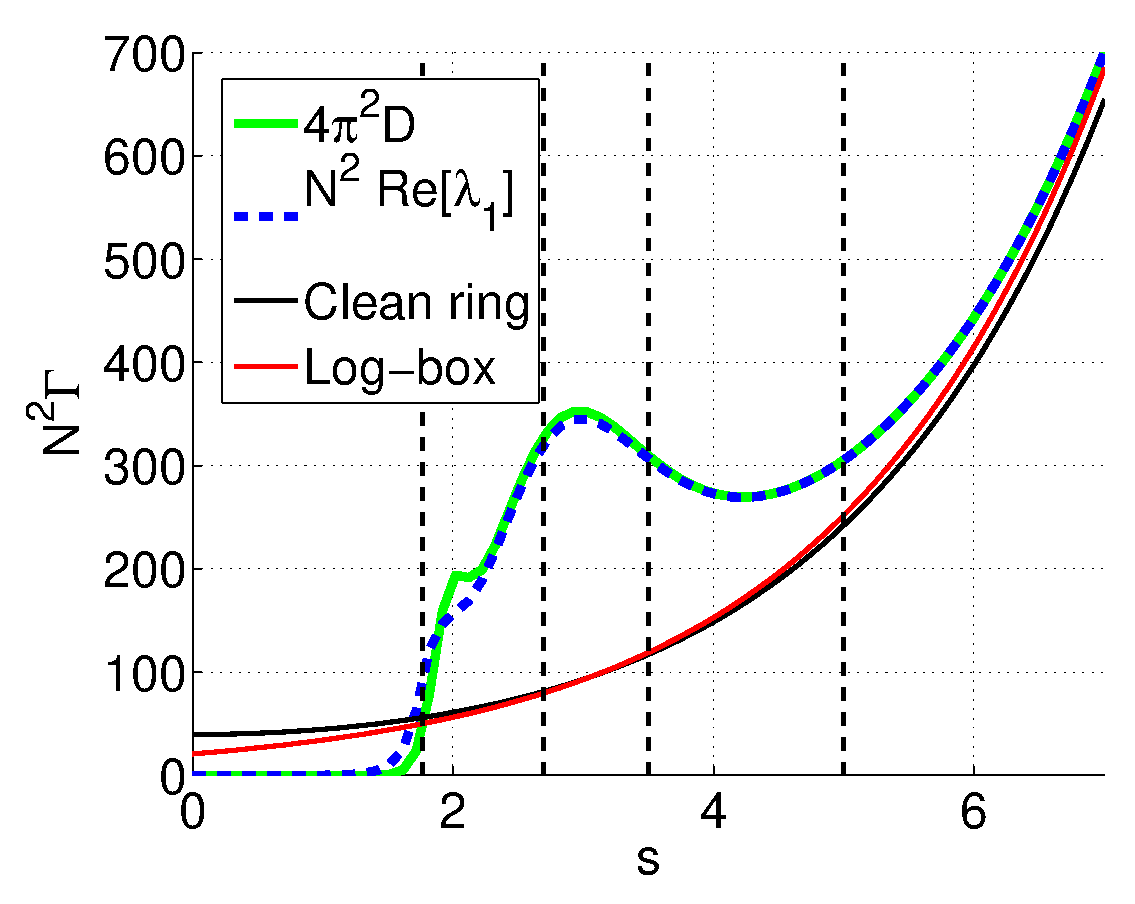
\includegraphics[height=6cm]{/Figs/gap_D_sigma5_N_1000.eps}
\caption{
The relaxation rate $\Gamma = \text{Re}[\lambda_1]$ versus the affinity $s$ for $N = 1000$ sites $\sigma = 5$. The non monotonic dashed blue line has been obtained via numerical diagonalization, whereas the solid green was obtained by calculating the diffusion coefficient as in \cite{nes}.
The monotonic lines correspond to the limits of
clean ring (\Eq{e13}, black) and $s>s_{\infty}$  (\Eq{e52}, red). The vertical dashed lines are the affinities 
$s_{\mu}$ that are associated with
the scaled values $\mu= 1/2, \ 1, \ 2, \ \infty$ (from left to right).}
%
%
%The real part of the gap of the complex spectrum $\Gamma = \text{Re}[\lambda_1]$ vs. $s$ for $N=1000$ sites and log-box field disorder with $\sigma=5$.
%The non monotonic dashed blue line was obtained by numerically diagonalization, 
%whereasthe solid green was obtained by calculating the diffusion coefficient as in \cite{nes}.
%The monotonic lines correspond to the limits if a clean ring \Eq{e13} (black) and $s>s_{\infty}$, \Eq{e52} (red).
%The vertical dashed lines from left to right are $s_{1/2},\  s_{1},\ s_{2}$ and $s_{\infty}$.    }t
\label{f1}
\end{figure}
%
\begin{figure}[h!]
 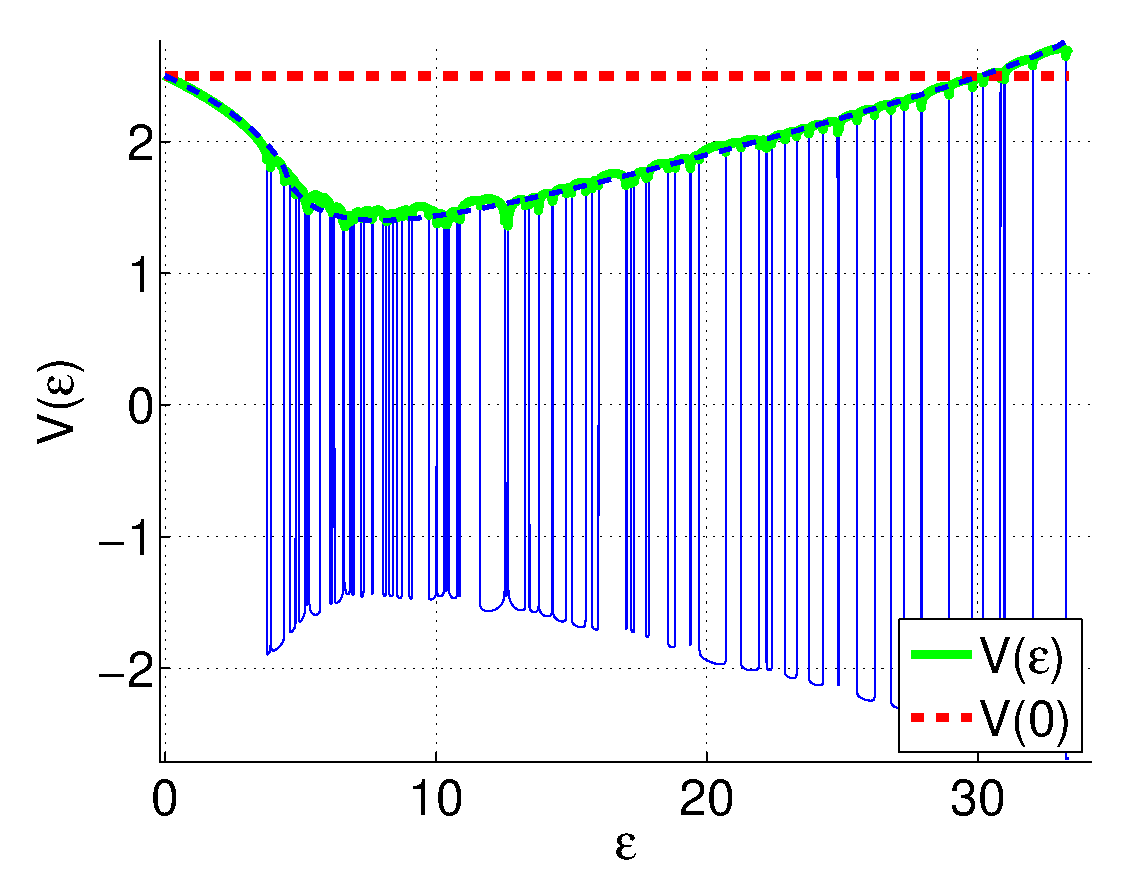
\includegraphics[width=6.2cm]{/Figs/V_E_s_inf}
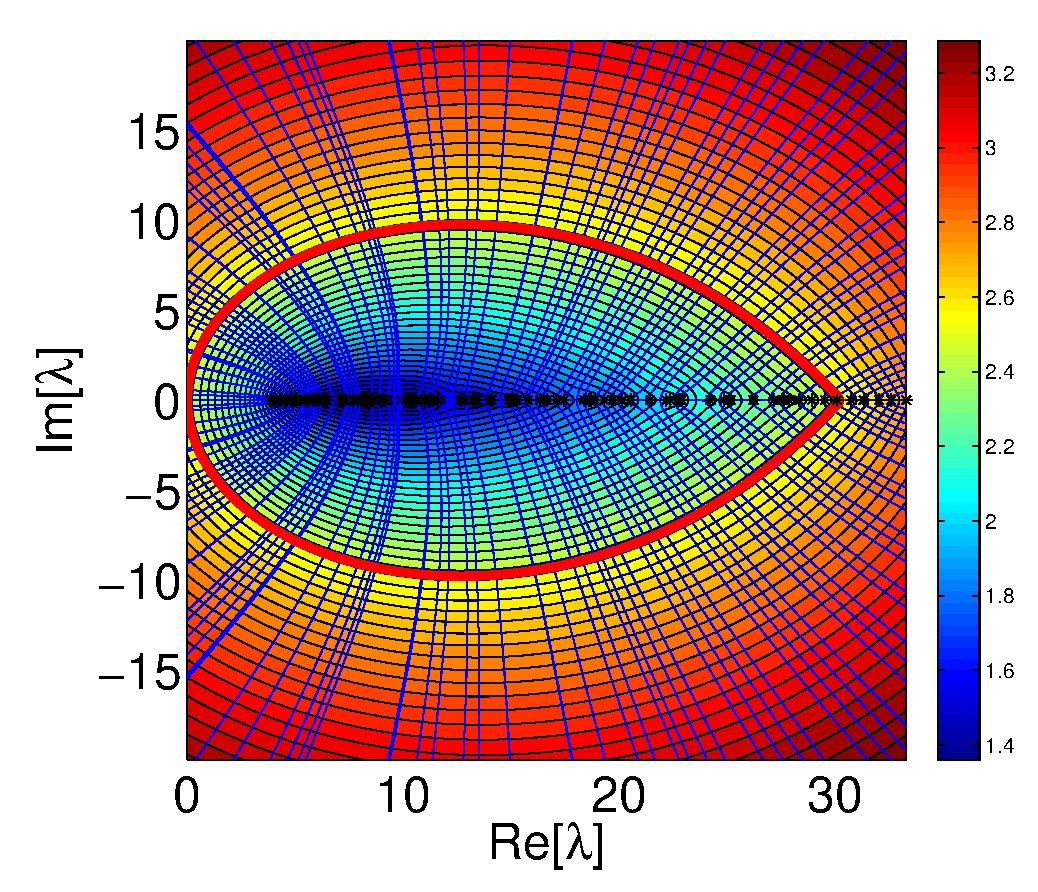
\includegraphics[width=7.5cm]{/Figs/electrostatics_large_S}
 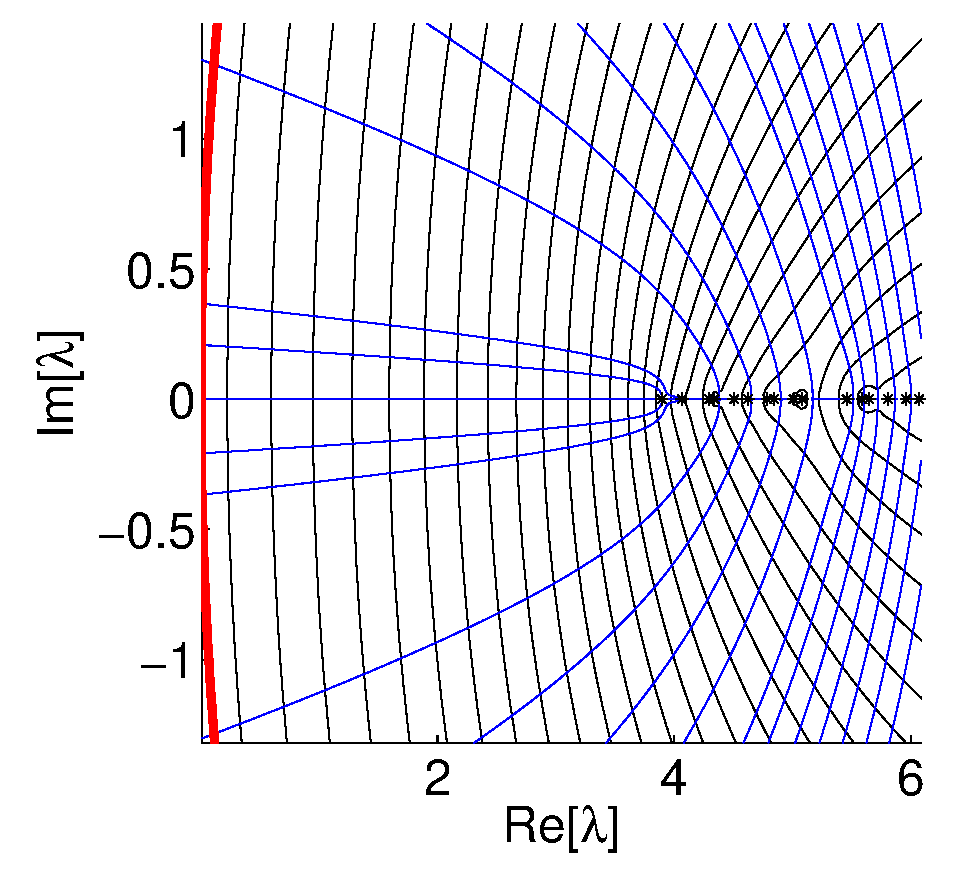
\includegraphics[width=7.5cm]{/Figs/electrostatics_large_S_zoom}

\caption{ {\bf Top panel}: The electrostatic potential $V(\epsilon)$ along the real axis. 
%The green points are the result of numerical diagonalization,
 The dashed blue line is the analytical result assuming $\rho=N(\sigma x)^{-1}$, \Eq{e43}. 
The stars 
indicate the position of the "charges", which are the eigenvalues of the associated Hermitian matrix, $\varepsilon_j$.
{\bf Middle panel}: 
The �electrostatic potential� $\Psi(z)$ of \Eq{e22}. Here we consider a ring with $N=100$
sites, $\sigma=2$ and $s=5$. The complex $\lambda_k$ spectrum is obtained by looking for the intersections of the field lineswith the red thick equipotential line $V(z)=V(0,0)$ that goes through the origin. 
%
{\bf Bottom panel}: Zoom. 
Note that the complex spectrum unlike the real spectrum does not have a gap.
%
%The red line is the equipotential line $V(\lambda) = V(0)$.
%The gap in the spectrum of $\bm{H}$  (black stars) is large, 
%but the real gap in the complex spectrum, (intersection
%of the contour $V=V(0)$and the first field line) diminishes as $1/N^2$.
%Here $N=100$ sites, $\sigma=2$ and $s=5$.
}
\label{figWeak}
\end{figure}

%%%%%%%%%%%%%%%%%%%%%%%%%%%%%%%%%%%%%%%%%%%%%%%%%%%%%%%%%%%%%%%%%
\section{Complexity saturation for $s \gg s_{\infty}$ }


The secular equation for the eigenvalues is given by \Eq{e20}.
%
In the nonconservative case, the eigenvalues of $\bm{H}$ do not depend on $s$,
 thus raising $s$ will eventually make the entire spectrum complex. 
For a conservative matrix, however, $V(\epsilon)$ is also a function of $s$, so increasing $s$ raises $V(\epsilon)$  at the same rate.
%
Due to the conservative property, the eigenvalues of the associated hermitian matrix, $\epsilon_j$ 
grow proportionaly to $e^s$. 
Increasing $s \to s+\Delta s$, we have
%
\beq
\sum_k \ln\left(\frac{z-\epsilon_k e^{\delta s}}{\overline{w}}\right)
&=&
 \ln \left[2\cosh\left(\frac{(s+\delta s)N}{2}\right) -2\right] \\
\sum_k \ln\left( \frac{z e^{-\delta s} - \epsilon_k}{\overline{w}}
 \right) 
 + N\Delta s &=&
 \ln \left[2\cosh\left(\frac{sN}{2}\right) -2\right] +N\delta s \ \ \ \ \ \ \ \ \
\eeq
%
but $z$ is just a dummy variable, so we can redefine $z := z e^{-\Delta s}$ and the equation is unchanged. Thus increasing $s$ does not change the number of complex solutions, as shown in \Fig{figCplxSat}.


%%%%%%%%%%%%%%%%%%%%%%%%%%%%%%%%%%%%%%%%%%%%%%%%%%%
To estimate the the saturation value of the fraction of complex eigenvalues, we assume $s \gg s_{\infty}$.
The eigenvalues have a log-box distribution so the potential along the real axis is 
%
\beq
V(\epsilon) \ \ &=& \ \  \int_a^b \ln|\epsilon - \epsilon'| \rho(\epsilon')d\epsilon'  =  \\
%\ \ &=& \ \ \int_{-\sigma}^{\sigma} \ln \left| e^{(s+\mathcal{E})/2} - e^{(s+\mathcal{E}_c)/2}\right| \rho(\mathcal{E})d\mathcal{E} = \\
\ \ &=& \ \ \frac{N}{2\sigma}\int_{-\sigma}^{\sigma} \ln \left| e^{(s+{\Delta}_c)/2} - e^{(s+\Delta)/2}\right| d\Delta
\eeq
%
Where we have defined the shifted stochastic field $\Delta = \mathcal{E}-s$  and 
 $\Delta_c$ such that the eigenvalues with $\Delta$ 
in the range ${-\sigma < \Delta < \Delta_c}$ are complex, $\Delta_c$ is determined by the equation ${V(\epsilon=e^{(s+\Delta_c)/2}) =  V(0) = sN/2}$, leading to 
%
\beq
\int_{-\sigma}^{\sigma} \ln \left| e^{{\Delta}/2} - e^{\Delta_c /2}\right| d\mathcal{E}  \ \ = \ \ 0 
\eeq
%
Clearly, $\Delta_c$ depends only on $\sigma$ (and not on $N$) (\Fig{figCplxSat}).
The fraction of complex eigenvalues  is just 
%
\be{101}
n =\frac{ \int_a^{\epsilon_c}  \frac{1}{ \epsilon} d\epsilon}{ \int_a^{b}  \frac{1}{ \epsilon} d\epsilon} = 
\frac{1}{\sigma}\ln\left( \frac{\epsilon_c}{a} \right) = 
\frac{\Delta_c + \sigma}{2\sigma}
\eeq
%


The percolation transition is reflected in the complexity saturation. 
If $\alpha \lesssim 1$ there is saturation, but the crossover is not as sharp and 
the saturation value is lower than \Eq{e101} and has a wider ensemble distribution.
This is demonstrated in the bottom panel of \Fig{figCplxSat}.
%
The argument for complexity saturation stems 
from the fact that for $s \gg s_{\infty}$ the matrix $\bm{H}$ is diagonal and the eigenvalues are trivially localized. 
If $w_n=1$ ($\alpha=\infty$), the eigenvalues are log-box distributed.
In the resistor network limit ($\sigma=0$ and finite $\alpha$), the eigenvalues are again trivially localized, but with the exponent derived in  \Sec{s8_1}. 
This leads to a lower saturation value that can be calculated by the same method used to derive \Eq{e101}.
In the general case where $\sigma \neq 0$ and $\alpha <\infty$, the calculation is more difficult, but it can be written formally as 
%
\beq
\int \ln \left(\epsilon_c-\gamma \right) P(\gamma) d\gamma \ = \ 0
\eeq
%
where $\gamma = w e^{\Delta/2}$, $w$ and $\Delta$ are random variables defined earlier and $P(\gamma)$ is the probability distribution of $\gamma$.
%
Generally, when $\alpha <\infty$ the couplings are no longer equal and can be very small,
thus for small $s$, $\bm{H}$ is no longer trivially localized and the eigenvalues have some complicated distribution. 
Specifically, the limits of the integral depend on the realization of disorder, which explains the dispersion of the saturation value from sample to sample.
%%%%%%%%%%%%%%%%%%%%%%%%%
\begin{figure}[h]
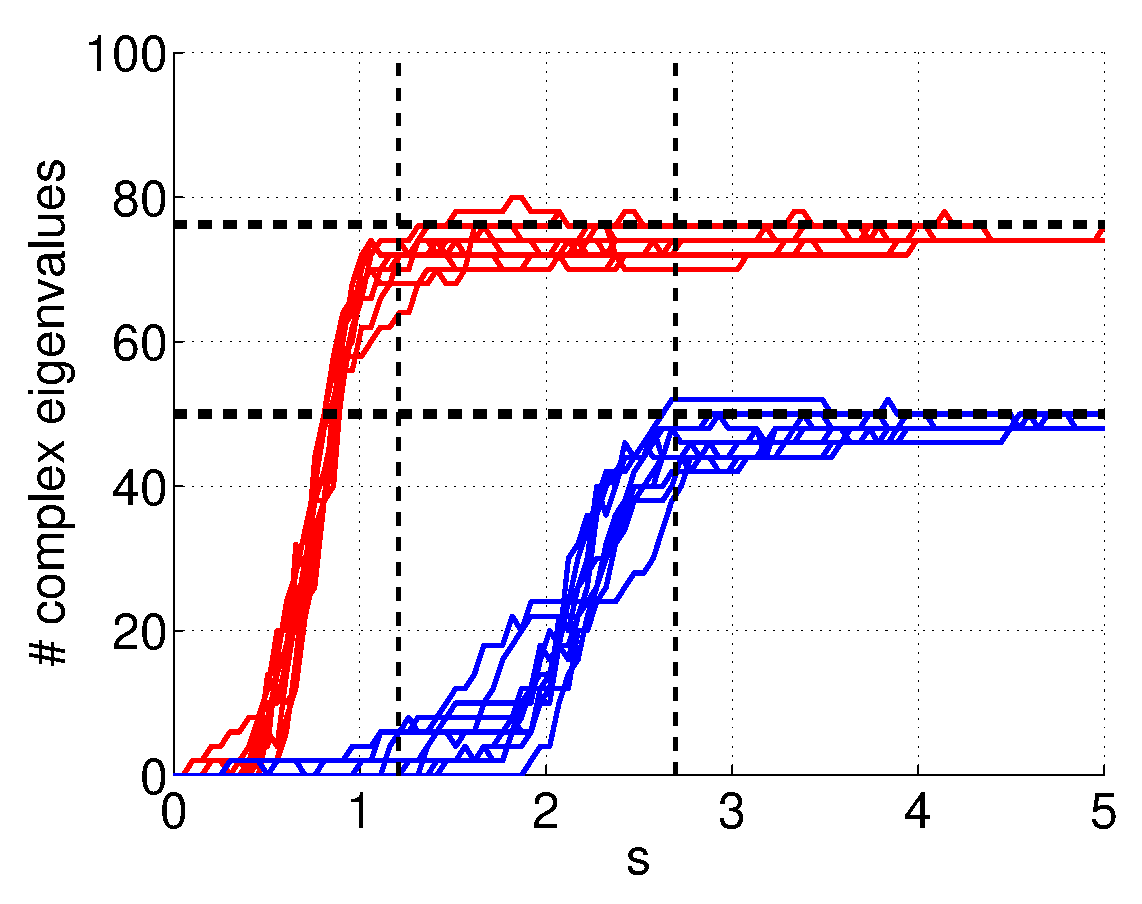
\includegraphics[height=5.4cm]{/Figs/numComplex_100}
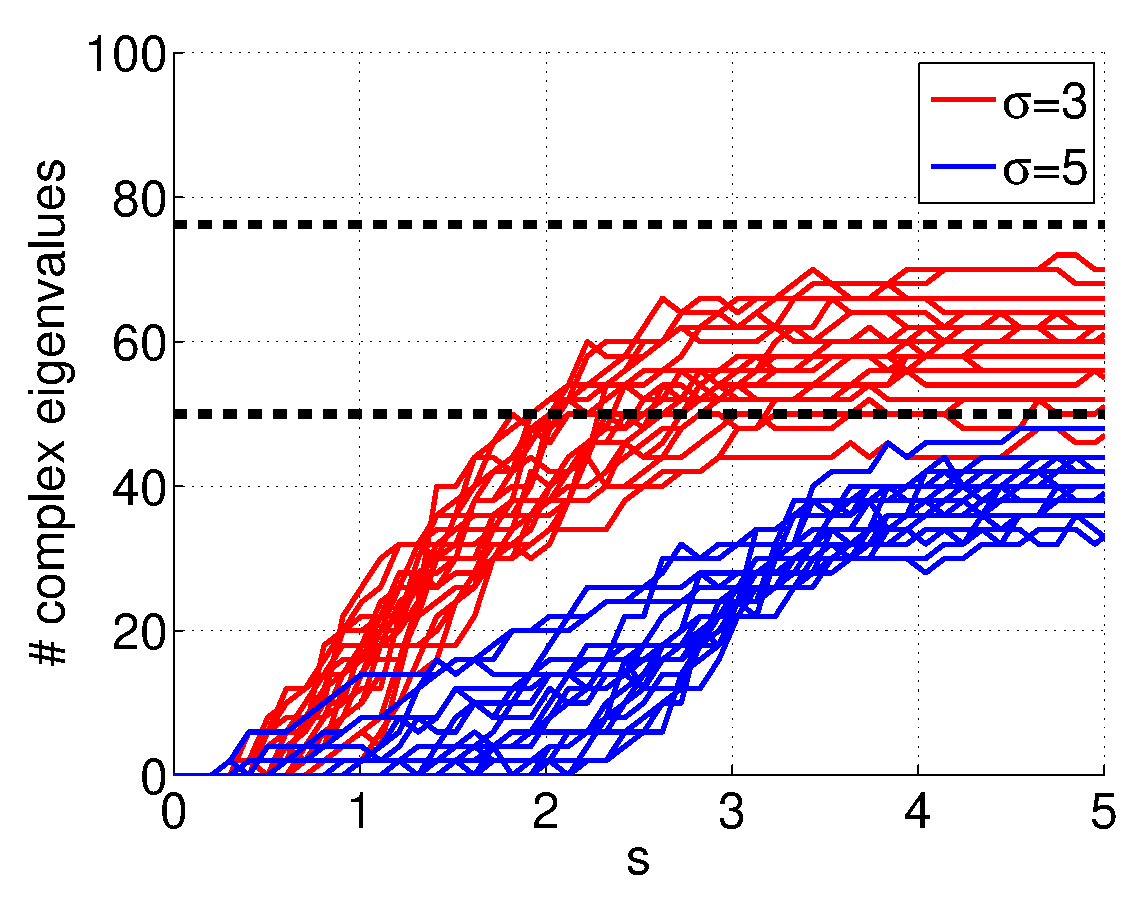
\includegraphics[height=5.4cm]{/Figs/numComplex_100_alpha}
%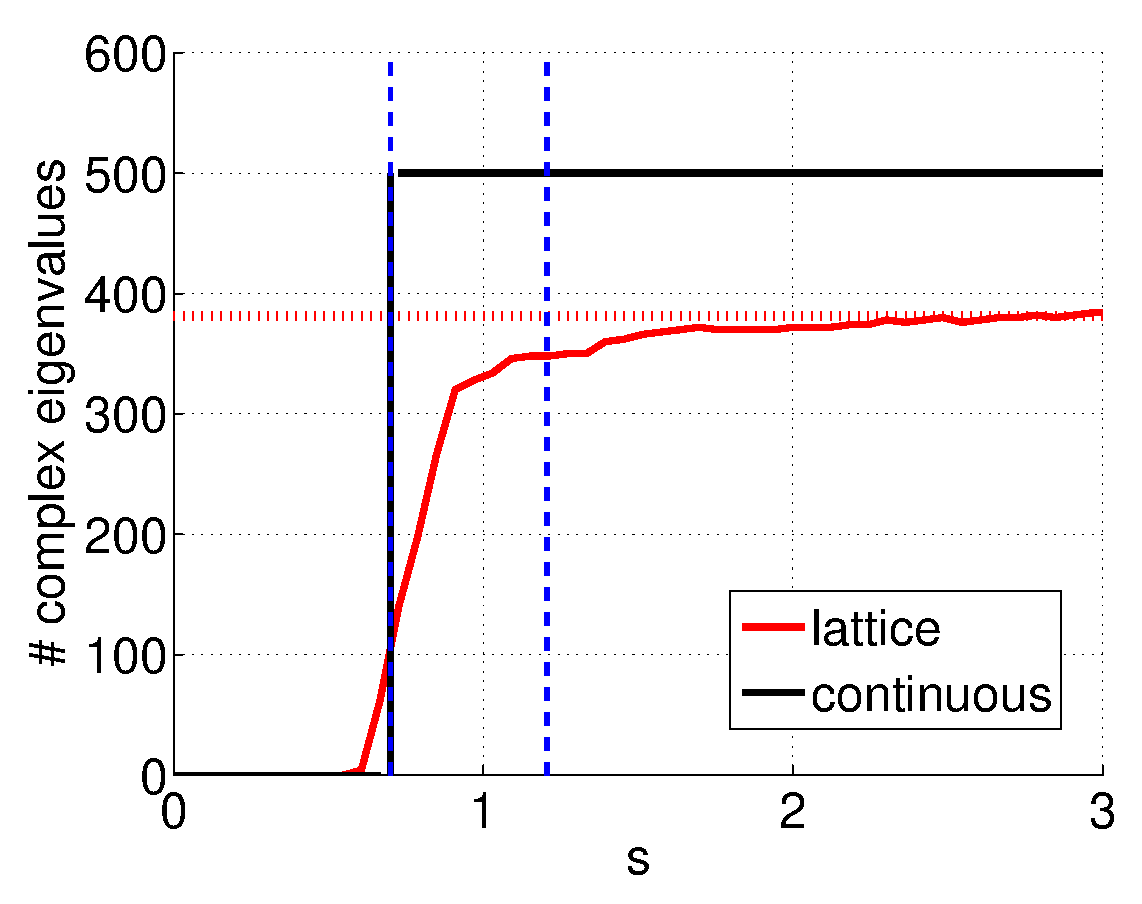
\includegraphics[height=5cm]{/Figs/numComplex_500}
\caption{
We count the number of complex eigenvalues
for a ring with $N=100$ sites, for various values of the affinity $s$. Each red line corresponds to a different
realization of field disorder with $\sigma=3$ (red) and $\sigma = 5$ (blue). 
The black vertical lines are at values of $s_1(\sigma)$
at which the sliding transition occurs. We see that the asymptotic fraction of complex eigenvalues saturates,
which is quite different from what is known for non-conservative non-Hermitian matrices. The horizontal
dashed line are analytical estimates of \Eq{e101}. 
If the lattice were continuous and the disorder white noise, the number of complex eigenvalues would 
go from 0 to 100 at $s=s_{1/2}$.
On the bottom panel $\alpha=0.9$, the crossover is blurred and the saturation value is lower (the horizontal lines are calculated for $\alpha=\infty$).
}
%Top: Number of complex eigenvalues vs. $s$ for $N=100$ sites. 
%Each red line corresponds to a different 
%realisation of field disorder with $\sigma=3$ (red) and $\sigma=5$ (blue), and $\alpha=\infty$. The black vertical lines are at values of $s_1(\sigma)$ at which the sliding transition occurs.
%Bottom: Number of complex eigenvalues vs. $s$ for $N=500$ sites and $\sigma=5$ (red)
%vs. the result of the continuous, white noise, problem (black step function). 
%The vertical dashed lines are $s_{1/2}$ and $s_1$. The dotted horizontal red line is the estimated saturation value, \Eq{e101}. 
\label{figCplxSat}
\end{figure}


%This explains the widening of the crossover and the dispersion of the saturation value.
%In the resistor network limit ($\sigma=0$), for very large $s$, $\bm{H}$ is again trivially localized with density of states $\rho \sim \epsilon^{\alpha-1}$, as explained in \Sec{s8_1}.

%
%%%%%%%%%%%%%%%%%%%%%%%%%%
%\begin{figure}[h]
%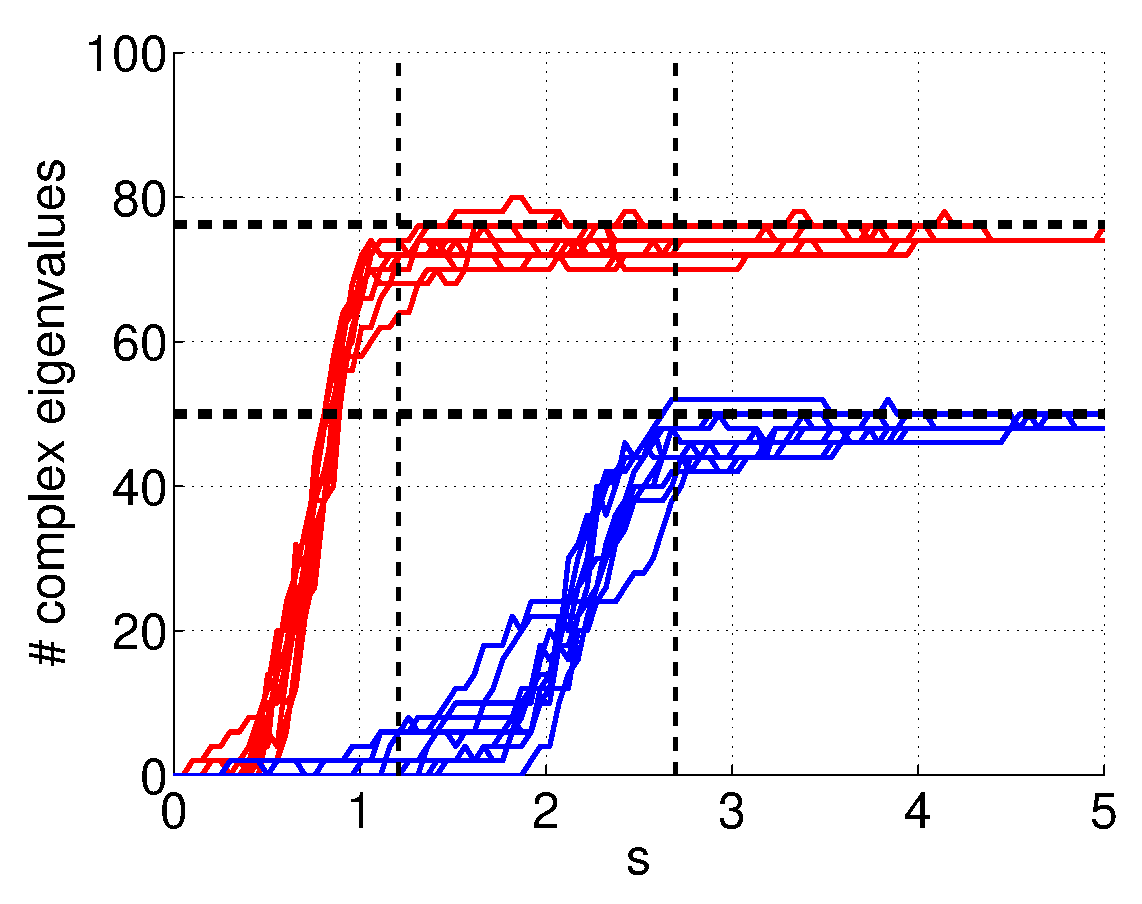
\includegraphics[height=5cm]{/Figs/numComplex_100}
%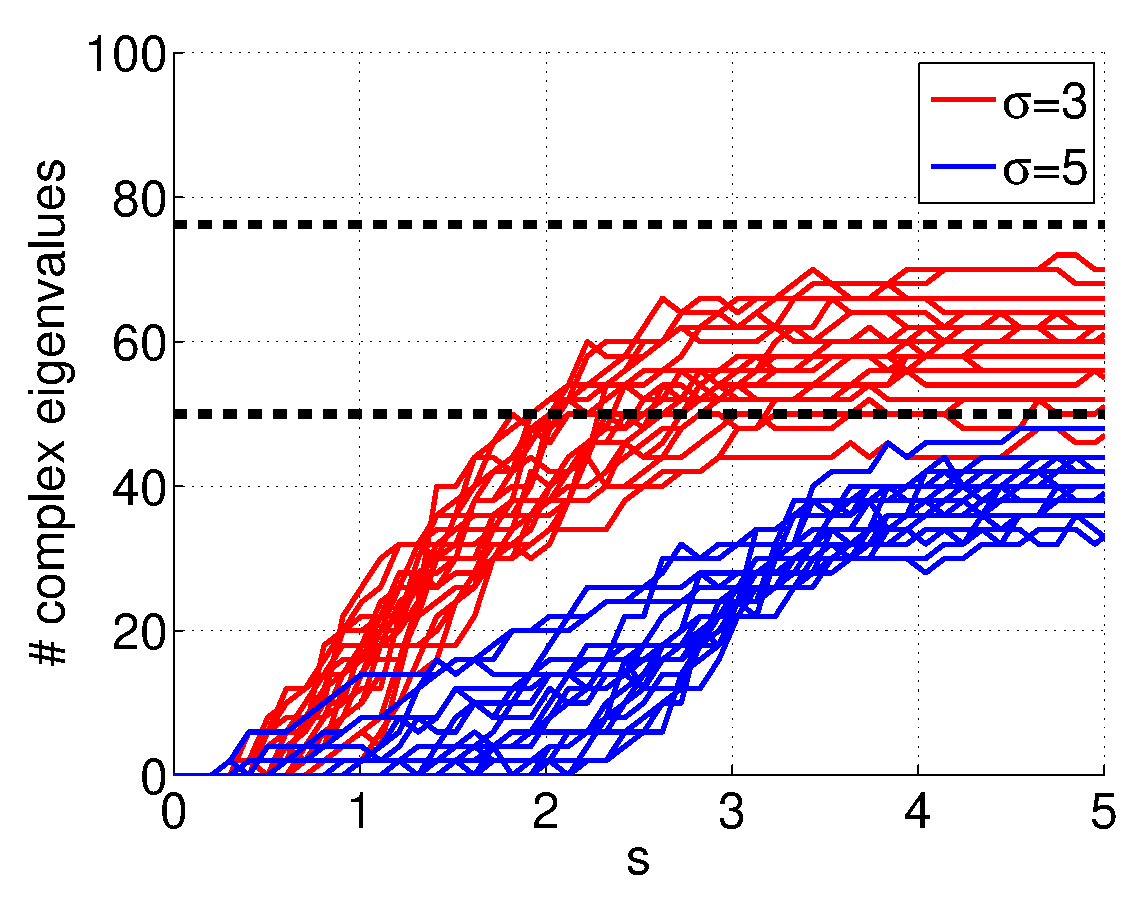
\includegraphics[height=5cm]{/Figs/numComplex_100_alpha}
%%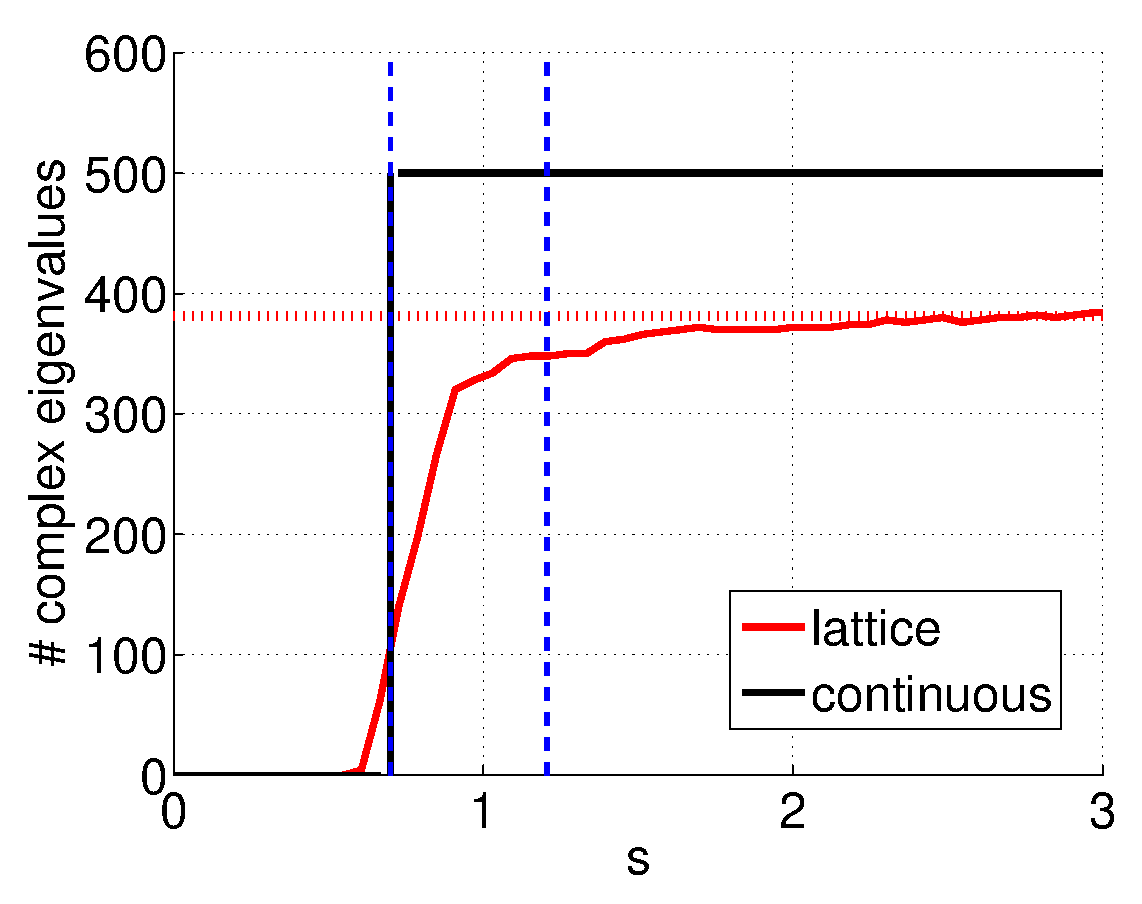
\includegraphics[height=5cm]{/Figs/numComplex_500}
%\caption{
%We count the number of complex eigenvalues
%for a ring with $N=100$ sites, for various values of the affinity $s$. Each red line corresponds to a different
%realization of field disorder with $\sigma=3$ (red) and $\sigma = 5$ (blue). 
%The black vertical lines are at values of $s_1(\sigma)$
%at which the sliding transition occurs. We see that the asymptotic fraction of complex eigenvalues saturates,
%which is quite different from what is known for non-conservative non-Hermitian matrices. The horizontal
%dashed line are analytical estimates of \Eq{e101}. 
%If the lattice were continuous and the disorder white noise, the number of complex eigenvalues would 
%go from 0 to 100 at $s=s_{1/2}$.
%On the bottom panel $\alpha=0.9$, the crossover is blurred and the saturation value is lower (the horizontal lines are calculated for $\alpha=\infty$).
%}
%%Top: Number of complex eigenvalues vs. $s$ for $N=100$ sites. 
%%Each red line corresponds to a different 
%%realisation of field disorder with $\sigma=3$ (red) and $\sigma=5$ (blue), and $\alpha=\infty$. The black vertical lines are at values of $s_1(\sigma)$ at which the sliding transition occurs.
%%Bottom: Number of complex eigenvalues vs. $s$ for $N=500$ sites and $\sigma=5$ (red)
%%vs. the result of the continuous, white noise, problem (black step function). 
%%The vertical dashed lines are $s_{1/2}$ and $s_1$. The dotted horizontal red line is the estimated saturation value, \Eq{e101}. 
%\label{figCplxSat}
%\end{figure}

%%%%%%%%%%%%%%%%%%%%%%%%%%%%%%%%%%%%%%%%%%%%%%%%%%%%%%%%%%%%
\section{Discussion}

To summarize \cite{brm2}, they use a different method, bypassing the hermitization procedure.
The long time behavior of $v$ and $D$ is deduced by numerical observations of the lower edge of the spectrum (small $|\lambda|$).
In fact the hermitization procedure is claimed to obscure the complexity transition (we found it!).
Somehow they do not bridge between complexity of the spectrum and the sliding transition in a purely conservative model. 
They make some comments regarding complexity and sliding in the following respect.
They consider a model where there are two types of unit cells. Each unit cell is made of two bonds.
The chain is composed of unit cells drawn from a bimodal distribution. 
Real eigenvalues only appear due to non conservative diagonal disorder  (detachment rate).
They do not find an explicit crossover to complexity and do not handle the purely conservative case.

\clearpage

%%%%%%%%%%%%%%%%%%%%%%%%%%%%%%%%%%%%%%%%%%%%%%%%%%%%%%%%%%%%%%%%%
\hide
{\section{Garbage}

\[ V(R) = \int_{0}^{x_c} \rho(x) \ln|x-R| dx \]

\[ V(R) = -\int_{0}^{x_c} \frac{(x/x_c)^{\mu}}{x-R} dx \]

More convenient to consider

\[ -\frac{1}{2} \int_{-u_c}^{u_c} \frac{ u^{2\mu+1} }{u^2-R} dx \]

For ${\mu=0}$ we recover the log potential of a point charge.
For ${\mu>0}$ the singularity is smeared and  ${V(0)}$ becomes finite.

\[ V(0) = - \frac{1}{\mu}  \]

In general ${x_c}$ is the border between the ${x^{\mu}}$ region 
and the "clean ring" region that extends up to the upper band edge.  
Accordingly ${V(0)}$ is shifted upwards.   

For ${\mu=1/2}$ we get  

\[V(R) = \{ (R/x_c)^{1/2}-1; \ \ \ \ -1(R>0) \} \] 

For general ${\mu}$ we need the derivative. 
For ${R<0}$ the calculation is straightforward

\[ V'(R<0) = -\int_{-u_c}^{u_c} \frac{ u^{2\mu+1} }{(u^2-R)^2} dx \]
 
leading to infinite slope at ${R=-0}$ for ${\mu<1}$.
Only for ${\mu>1}$ the left slope ${V'(-0)}$ becomes finite and continuous.

The expressions for ${V'(+0)}$ required regolarization in the regime ${R>0}$, 
leading for any ${\mu}$ to a finite-slope result

\[ V'(+0) = -\Gamma(2\mu-2) \frac{1}{x_c} \]

For Math see

Computing the Hilbert Transform of the Generalized Laguerre and Hermite Weight Functions 
http://link.springer.com/article/10.1023%2FA%3A1021915128433

The slope change sign at ${\mu=1/2}$, 
hence for ${\mu>1/2}$ the minimum of ${V(R)}$ is to the right of ${R=0}$. 
 }


%%%%%%%%%%%%%%%%%%%%%%%%%%%%%%%%%%%%%%%%%%%%%%%%%%%%%%%%%%%%%%%%%%%%%%%%%%%%%%%%%%%%
%%%%%%%%%%%%%%%%%%%%%%%%%%%%%%%%%%%%%%%%%%%%%%%%%%%%%%%%%%%%%%%%%%%%%%%%%%%%%%%%%%%%
\clearpage
\bibliography{neg_bib.bib}{}
%\bibliographystyle{ieeetr}


%%%%%%%%%%%%%%%%%%%%%%%%%%%%%%%%%%%%%%%%%%%%%%%%%%%%%%%%%%%%%%%%%%%%%%%%%%
%%%%%%%%%%%%%%%%%%%%%%%%%%%%%%%%%%%%%%%%%%%%%%%%%%%%%%%%%%%%%%%%%%%%%%%%%%

\section*{Acknowledgements}

This research has been supported by  by the Israel Science Foundation (grant No. 29/11).


\hidea{
\section*{Author contributions statement}

Both authors have contributed to this article. 


\section*{Additional information} 

% Reprints and permissions information is available at www.nature.com/reprints\\
The authors declare that they have no competing financial interests.
% Correspondence and requests for materials should be addressed to avardi@bgu.ac.il or dcohen@bgu.ac.il

}
%%%%%%%%%%%%%%%%%%%%%%%%%%%%%%%%%%%%%%%%%%%%%%%%%%%%%%%%%%%%%%%%%%%%%%%%%%
%%%%%%%%%%%%%%%%%%%%%%%%%%%%%%%%%%%%%%%%%%%%%%%%%%%%%%%%%%%%%%%%%%%%%%%%%%
\clearpage
\appendix  
\onecolumngrid


\section{ Finding the sign of $V'(0)$}
\label{A1}

To derive \Eq{e19} we assume an integrated density of states corresponding to \Eq{e3}, 
${\mathcal{N}(\epsilon) = (\epsilon/\epsilon_c)^{\mu}}$, where $\epsilon_c$ is some cutoff due to the discreteness of the lattice.
The electrostatic potential along the real axis is given by (integration by parts of \Eq{e23})
%
\beq
V(\epsilon) &=& -  \int_0^{\epsilon_c} \frac{\mathcal{N}(x)}{x-\epsilon}dx
\eeq
and the derivative with respect to $\epsilon$ at the origin is (after integrating by parts)
%
\beq
V'(\epsilon) \ \ &=& \ \ \int_0^{\epsilon_c} \frac{\mathcal{\rho}(x)}{x-\epsilon}dx = \\
\ \ &=& \ \   \frac{\mu}{\epsilon_c^{\mu}}\int_0^{\epsilon_c} \frac{x^{\mu-1}}{x-\epsilon}dx \ =  \\
&=&\frac{\mu}{\epsilon_c^{\mu}} \epsilon^{\mu-1} \int_0^{z_c} \frac{z^{\mu-1}}{z-1}dz = 
 \frac{\mu}{\epsilon_c^{\mu}}  \epsilon^{\mu-1}I(\epsilon) = \rho(\epsilon) I(\epsilon)
\eeq
%
where we substituted $z=x/\epsilon$ and defined
%
\beq
I(\epsilon) = \int_0^{z_c} \frac{z^{\mu-1}}{z-1}dz \  , \ \ \ z_c=\frac{\epsilon_c}{\epsilon}
\eeq
%
The integral converges for ${\mu<1}$. 
The integral can be written in terms of Incomplete Euler Beta functions defined as 
%
\beq
B_u(a,b) = \int_0^u x^{a-1}(1-x)^{b-1}dx
\eeq
%
However one must be careful and take only the Cauchy principal part
\beq
\!\!\!\! \lim_{\epsilon \to 0} I  &=& \lim_{\epsilon \to 0}  \int_0^{z_c}\frac{z^{\mu-1}}{z-1}dz =\\
\!\!\!\! & \ \ = \ \ &\lim_{\epsilon \to 0}  \lim_{\delta \to 0} \left[ \int_0^{1-\delta}x^{\mu-1}(1-z)^{-1}dz + 
\int_{1+\delta}^{z_c} z^{\mu-1}(1-z)^{-1}dz \right]= \\
&=&\lim_{\epsilon \to 0}  \lim_{\delta \to 0}  \left[ B_{1-\delta}(\mu,0) + 
\int_{1+\delta}^{z_c} z^{\mu-1}(1-z)^{-1}dz \right]\\
&=&\lim_{\epsilon \to 0}  \lim_{\delta \to 0}  \left[ B_{1-\delta}(\mu,0) - 
\int_{1/z_c}^{1-\delta} t^{-\mu}(1-t)^{-1}dx \right]\\
&=&\lim_{\delta \to 0}  \left[ B_{1-\delta}(\mu,0) - B_{1-\delta}(1-\mu,0) \right] = \\
&=& \psi(1-\mu)-\psi(\mu) = \pi \cot(\pi \mu)
\eeq
%
where $\psi(z)$ is the digamma function and the last equality was obtained by the reflection formula. 
%
To go from the fourth to the fifth line  we took the limit $z_c=\to \infty$, which corresponds to $\epsilon\to0$.
%
It is clear that $C$ and thus $V'(0^+)$ changes sign from positive to negative at $\mu=1/2$.\\
%
%\beq
%V'(0^+) =\lim_{R\to 0^+} \frac{ R^{\mu}}{x_c^{\mu}} \pi\mu \cot(\pi \mu)
%\eeq

%%%%%%%%%%%%%%%%%%%%%%%%%%%%%%%%%%%%%%%%%%%%%%%%%%%%%%%%
\section{Sliding transition - the definition of $s_{\mu}$}
\label{A2}

In order to understand the dependence of $v$ and $D$ on $N$ and $s$, 
it is useful to recall known results that have been obtained 
for the time-dependent spreading in an $N=\infty$ lattice.
Recall that the drift is induced by the stochastic field, \Eq{e6}
whose affinity is defined
%
\beq
s = \frac{1}{N}\sum_{n=1}^N \mathcal{E}_{n}
\eeq
%
The cummulant generating function of the stochastic field 
can be written as $g(\mu)=(s-s_{\mu})\mu$, where $s_{\mu}$ 
is defined via the following expression:   
%
\be{362}
\left\langle  e^{-\mathcal{E}\mu}\right\rangle \ \ \equiv \ \ \eexp{-(s-s_{\mu})\mu} 
\eeq
%  
If the stochastic field has normal distribution 
with standard deviation $\sigma$, then ${s_{\mu}=(1/2) \sigma^2 \mu}$.
For our box distribution with $\mathcal{E} \in [s-\sigma,s+\sigma]$,
%
\beq
s_{\mu}  \ \ = \ \ \frac{1}{\mu} \ln\left( \frac{\sinh (\mu \sigma)}{\mu \sigma} \right)
% \frac{ \sinh (\mu \sigma)}{\mu \sigma} \ \eexp{-\mu s}  \ \ = \ \ 1
\eeq
%
which is monotonically ascending from zero to $s_{\infty} = \sigma$. 
The positive monotonic function $s_{\mu}$ can be inverted,
hence we can define a scaled affinity $\mu(s)$.
Note that \Eq{e362} implies that $\mu(s)$ is the value 
of $\mu$ for which the left-hand-side equals unity. 
%

It has been shown in \cite{odh1} that the velocity (first moment) exhibits a transition at $s_1$ from zero to finite velocity. 
The diffusion (second moment) at $s_2$ goes from finite to divergent.
In the text we showed that the delocalization transition occurs at $s_{1/2}$, 
which also corresponds to the diffusion coefficient going from sub-ohmic to super-ohmic \cite{nes}.

\section{The Poisson limit}
\label{A11}

In \cite{nes} we have shown that the diffusion coefficient in the large $s$ limit is given by
%
\beq
D(s>s_{\infty}) &=&  \frac{N^2}{2} \left[\left( \sum_{n=1}^N \frac{1}{w_n} \right)^{-3} \left(\sum_{n=1}^N \frac{1}{w_n ^2}\right)\right] \\
&=& \frac{1}{2} \left\langle \frac{1}{w}\right\rangle ^{-3}   \left\langle \frac{1}{w^2}\right\rangle = \\
&=&  \frac{1}{2}\frac{\sigma^2}{4} \frac{\cosh(\sigma/2)}{\sinh^2(\sigma/2)}e^{s/2} = \frac{1}{2}\cosh\left(\frac{\sigma}{2}\right) \exp\left(\frac{s-s_{1/2}}{2}\right)
\eeq
%
where we transformed to an integral $\sum_n \to \int \rho(\mathcal{E}) d\mathcal{E}$.
%For a log-box distribution of transition rates, $w_n = e^{\mathcal{E}/2}$, $\mathcal{E} \sim [s-\sigma, s+\sigma]$ we obtain 
%%
%\beq
%D = 
%\eeq
%%


\section{ The similarity transformation (definition of H)} 
\label{A3}

The associated hermitian matrix ${\bm H}$ is obtained by a similarity transformation to a basis in 
which the stochastic field is uniform $\epsilon=s$, followed by setting $s=0$ on the off diagonals.
%
\beq
{\bm W}
&=&
\left(
\begin{array}{cccccc}
-\gamma_1 & w_1 e^{\mathcal{E}_1/2}& & w_N e^{-\mathcal{E}_N/2} \\
w_1 e^{-\mathcal{E}_1/2} & \ddots & \ddots&  & & \\
 & \ddots & \ddots & w_{N-1} e^{\mathcal{E}_{N-1}/2}\\
w_n e^{\mathcal{E}_N/2} & &w_{N-1} e^{-\mathcal{E}_{N-1}/2} & -\gamma_N
\end{array}
\right)
\eeq
%
where the decay rates are determined by conservativity
%
\beq
\gamma_n = w_{n-1}e^{-\mathcal{E}_{n-1}/2} + w_{n} e^{\mathcal{E}_n/2}
\eeq
%
The following similarity transformation 
%
\be{3000}
\left\{e^{{-\bm V}/2} \right\}_{ij}& = & \delta_{ij}\exp\left[ -\frac{1}{2}\sum_{k=1}^{j-1} \mathcal{E}_k \ + \frac{j-1}{2}\bar{s}\right], \\
\bar{s} & =  & \frac{1}{N}\sum_{k=1}^N \mathcal{E}_k
\eeq
%
reduces the rate equation to 
%
\beq
{\bm \tilde{W}} = e^{{\bm V/2}} W e^{-{\bm V/2}} &=&
\left(
\begin{array}{cccccc}
-\gamma_1 & w_1 e^{\bar{s}/2}& & w_N e^{-\bar{s}/2} \\
w_1 e^{-\bar{s}/2} & \ddots & \ddots&  & & \\
 & \ddots & \ddots & w_{N-1} e^{\bar{s}/2}\\
w_n e^{\bar{s}/2} & &-w_{N-1} e^{-\bar{s}/2} & -\gamma_N
\end{array}
\right)
\eeq
%
The associated hermitian matrix is defined by setting $\bar{s}=0$,
%
\beq
{\bm H} &=&
\left(
\begin{array}{cccccc}
-\gamma_1 & w_1& & w_N\\
w_1  & \ddots & \ddots&  & & \\
 & \ddots & \ddots & w_{N-1}\\
w_n  & &-w_{N-1}  & -\gamma_N
\end{array}
\right)
\eeq
%
which is of course real, symmetric and has real eigenvalues $\epsilon_k$.

\subsection{Definition of conservative property}

Most commonly, a conservative matrix is defined such that each column of the matrix sums to zero. 
In the previous section we showed that a conservative matrix ${\bm W}$ can be transformed 
by a similarity transformation to a seemingly non conservative matrix ${\bm H}$, whose columns do not sum to zero. 
So we ask, what properties must ${\bm H}$ have to represent a conservative hopping process?
It turns out that ${\bm H}$ is similar (by similarity transformation) to a conservative ${\bm W}$ if and only if 
${\bm H}$ can be written as $AA^{\dag}$, where $A$ is a lowering operator defined as 
%
\beq
A |n\rangle = \sqrt{w_n} \left[ e^{-\mathcal{E}_n/4} |n \rangle + e^{\mathcal{E}_n/4} |n-1 \rangle \right]
\eeq
%
Then $H=AA^{\dag}$ describes a hopping process with rates $w_n$ 
and on site energies $\gamma_n$
%
\beq
\gamma_n =w_n e^{-\mathcal{E}_n/2}+w_{n+1} e^{-\mathcal{E}_{n+1}/2}
\eeq
%
Then, by the similarity transformation of \Eq{e3000} (considering the case of $\bar{s}=0$)
%
\beq
{\bm W} = e^{-V/2} {\bm H} e^{V/2}
\eeq
%
describes a conservative stochastic process with rates $w_n e^{\pm \mathcal{E}_n/2}$ and NESS $p_n \propto e^{-V_n}$.

\section{The formula for the spectral determinant}

For the purpose of this section it makes things easier to define ${\bm \Gamma} = -{\bm W}$, the goal is 
to derive an expression for the spectral determinant 
%
\beq
\det ( {\bm\Gamma} - \lambda {\bm I})   = 0
\eeq
%
in terms of the hermitian eigenvalues $\epsilon_k$.
This determinant can be calculated using a formula due to Molinari \cite{det1} for tridiagonal matrices. 
We define the matrix 
%
\beq
T_n &=& \left(
\begin{array}{cc}
 \gamma_{n} -\lambda& -w_{n-1}^2 \\
1 & 0
\end{array}
\right)
\eeq
%
The key point is that the matrices $T_n$ are the same for ${\bm\Gamma}$ and for ${\bm H}$. 
Using the formula for the deteminant for both matrices, we obtain
%
\beq
\det \left( {\bm H} - \lambda \bm{I} \right) &=&  \mathrm{tr}  \left[\prod_{n=1}^N T_n\right] - 2 \left[ \prod_{n=1}^N w_n \right]  \\
\det \left( {\bm \Gamma} - \lambda {\bm I} \right) &=&  \mathrm{tr}  \left[\prod_{n=1}^N T_n\right] - 2 \left[ \prod_{n=1}^N w_n \right] \cosh\left(\frac{N\bar{s}}{2}\right)\\
\eeq
%
subtracting the equations and writing the characteristic polynomial of the Hermitian matrix 
%
\beq
\det \left( {\bm H} - \lambda \bm{I} \right) \ = \ \prod_{n=1}^N \left(  \epsilon_n - \lambda\right) 
\eeq
%
we obtain an equation for the eigenvalues $\lambda$ (\Eq{e17})
%
\beq
 \prod_{n=1}^N \left(  \lambda - \epsilon_n \right)  \ = \   \left[\prod_{n=1}^N w_n\right]  2\left(\cosh\left(\frac{N\bar{s}}{2}\right) -1\right)
\eeq
%

According to Thouless, for the corresponding Hermitian problem
%
\beq
e^{ N / \xi} = \prod_{n=1}^N{ \left(\frac{  \epsilon - \epsilon_n }{  w_n }\right)}
\eeq
%
where $\xi(\epsilon)$ is the energy dependent  localization length.

\section {Clean ring}
\label{A4}

The real spectrum of a clean ring is doubly degenerate, see \Fig{figClean}. The spectrum is completely complex.
The potential oscillates and does not reach the "cosh line" and appears to have $N/2$ maxima. 
Introducing a small perturbation to one of the bonds, say $g=1-\varepsilon$ removes the degeneracy and
raises the remaining maxima from $-\infty$.

\begin{figure}[h]
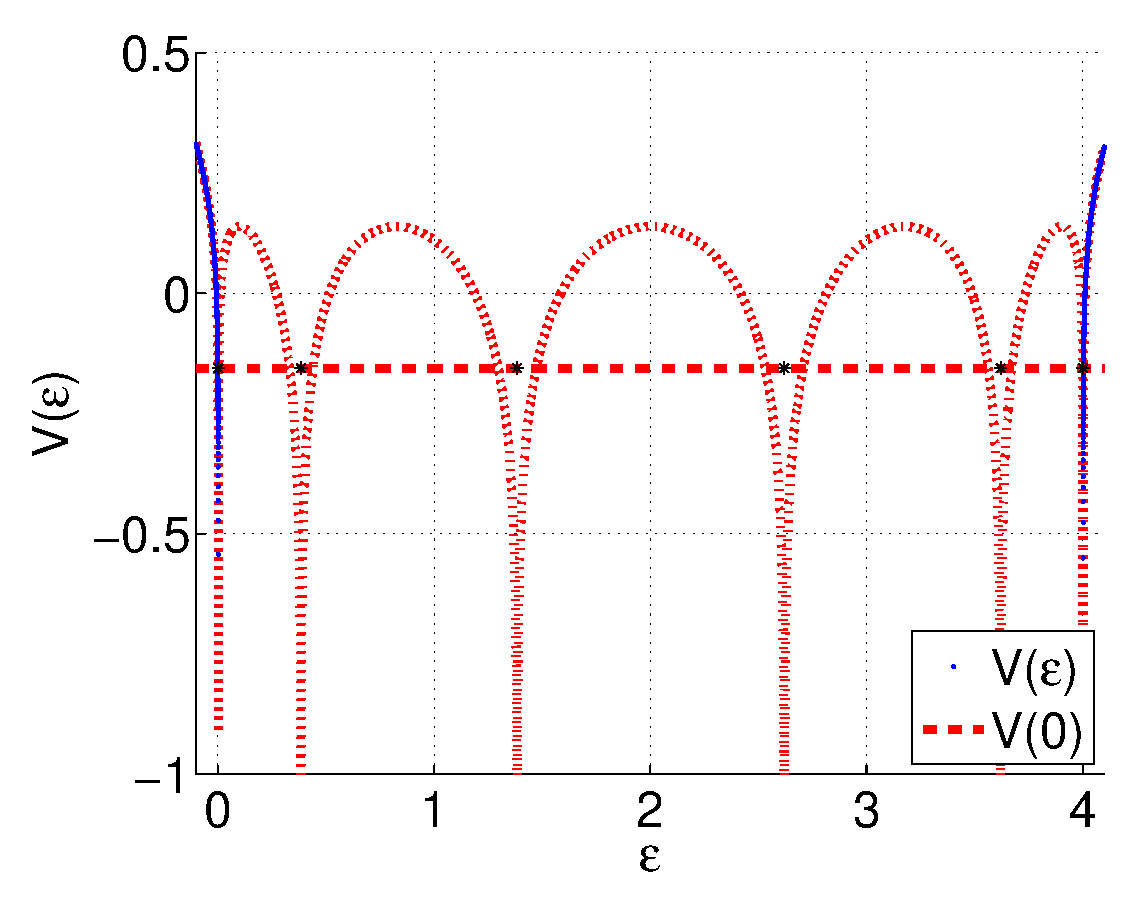
\includegraphics[height=5cm]{/Figs/V_clean_1}
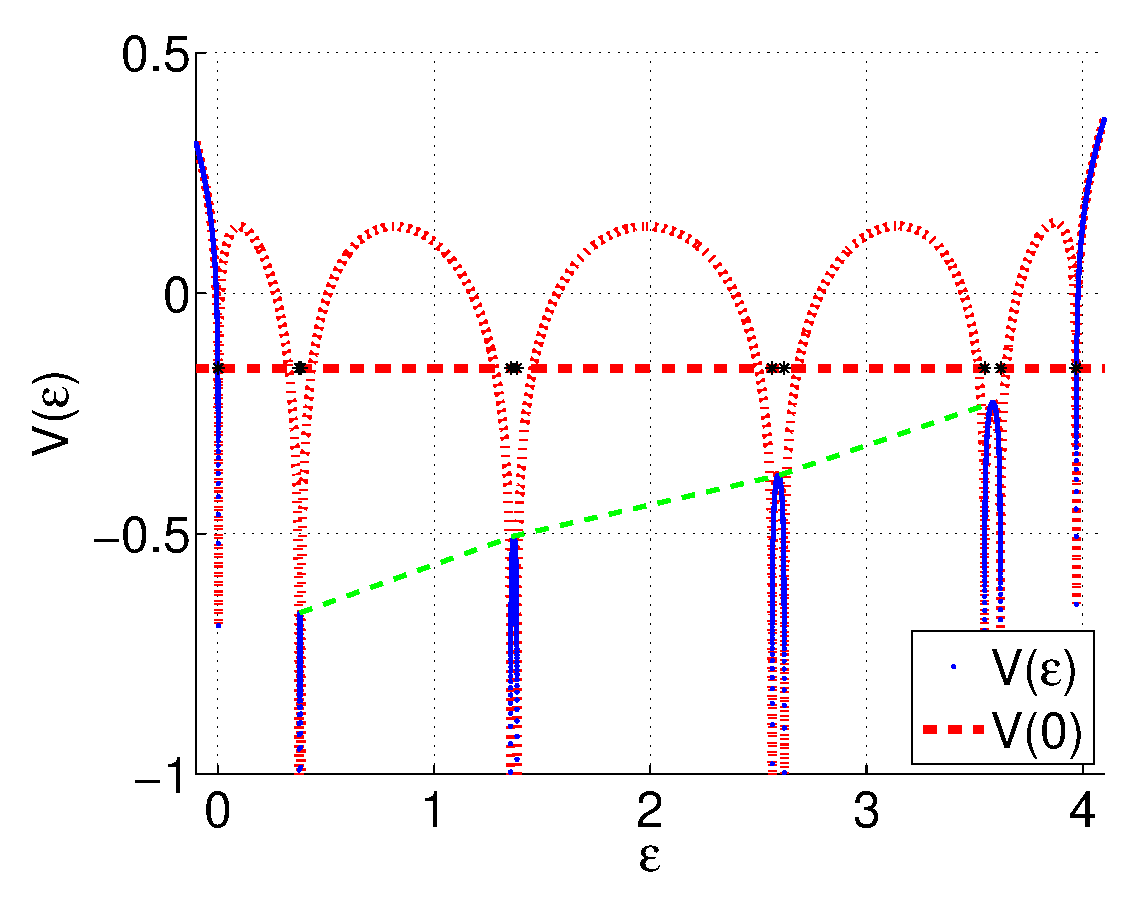
\includegraphics[height=5cm]{/Figs/V_clean_2}
\caption{Solving the secular equation for a clean ring. 
The left panel shows the electrostatic potential of a clean ring, which is doubly degenerate. 
In the right panel one of the bonds is perturbed. Here $N=10$ and $g=0.9$ and $s=0.1$
}
\label{figClean}
\end{figure}

\section{Continuous ring}
\label{A5}

The purpose of this appendix is to derive the secular equations for the continuous version of a weak link and a stochastic field defect. 
The derivation is based on the transfer matrix method applied to the diffusion equation. 
We first present the transfer matrix method applied to the diffusion equation.
In the following sections we introduce the matching conditions for piecewise constant $D(x)$ and $u(x)$ which are used to construct a weak link and a stochastic field defect.  

The dynamics of the continuous limit is described by a diffusion equation
with spatially dependent diffusion coefficient $D(x)$ and drift velocity $u(x)$
%
\be{1011}
\frac{\partial \psi}{\partial t} &=&\frac{\partial}{\partial x} \left[ D(x) \frac{\partial \psi}{\partial x}-u(x)\psi\right] 
\ = \ \frac{\partial}{\partial x} \left[ D(x) \frac{\partial \psi}{\partial x}\right] -
 \frac{\partial}{\partial x} \left[u(x)\psi\right] 
\eeq
%
Assuming that $D(x)$ and $u(x)$ are piecewise constant, the 
solution to the diffusion equation in each region is  simply  $\psi \sim e^{-\lambda t + ikx}$, inserting this in \Eq{e1011}, we obtain the dispersion relation 
%
\beq
\lambda &=& Dk^2 + iuk \ = \ D\left(k+\frac{iu}{2D}\right)^2 + \frac{u^2}{4D} \\
k_{\pm} &=& \frac{-iu \pm \sqrt{4\lambda D -u^2}}{2D} = \frac{-is}{2} \pm \sqrt{\frac{\lambda}{D}-\frac{s^2}{4}} \\
\ \ & \equiv & \ \   \frac{-is}{2} \pm \tilde{k}
\eeq
%
So, in each region the solution to \Eq{e1011} is a superposition of clock wise ($k_+$) and counterclockwise ($k_-$) waves
%
\be{1012}
\psi(x)  &=&  Ae^{ik_{+} x}+ Be^{ik_{-} x} = \\
& = & \eexp{\frac{u}{2D}x} \left(Ae^{i\frac{\sqrt{4\lambda D -u^2}}{2D}x}+Be^{-i\frac{\sqrt{4\lambda D -u^2}}{2D}x}\right) = \\
& = & \psi^{+}(x) + \psi^{-}(x)
\eeq
%
From now on we replace $\tilde{k} \to k$.
We define the vector 
%
\beq
\left( \begin{array}{c}
\psi ^+ (x)\\
\psi ^- (x)
\end{array}
\right)
\eeq
%
In the next section it will be more convenient to work with the vector 
%
\beq
\left( \begin{array}{c}
\psi \\
\partial \psi
\end{array}
\right) =  
\left(
\begin{array}{cc}
 1 & 1 \\
ik_+ & ik_- \\
\end{array}
\right)
\left( \begin{array}{c}
\psi ^+ (x)\\
\psi ^- (x)
\end{array}
\right)
\eeq
%
The transfer matrix is along a distance $x$ is $UT(x)U^{-1}$ where
%
\beq
U = \left(
\begin{array}{cc}
 1 & 1 \\
ik+\frac{i s}{2} & -ik+\frac{i s}{2} \\
\end{array}
\right)
\eeq
and 
%
\beq
T = \left(
\begin{array}{cc}
 e^{i \left(k-\frac{i s}{2}\right) x} & 0 \\
 0 & e^{i \left(-k-\frac{i s}{2}\right) x} \\
\end{array}
\right)
\eeq
%
such that for a segment of length $L$
%
\beq
\left.\left( \begin{array}{c}
\psi \\
\partial \psi
\end{array}
\right)\right|_{x=0}  \ \ = \ \ UT(L)U^{-1}
\left.\left( \begin{array}{c}
\psi \\
\partial \psi
\end{array}
\right)\right|_{x=L} 
 \eeq
 %
 
\section{ Ring with weak link "$g$"}
\label{A6}

The purpose of this section is to derive \Eq{e51}, which is the condition for complexity 
in a ring with a weak link, in the continuum limit.
The ring has circumference $L$ and a weak link, which is a small region $|x|<a/2$ where the diffusion
coefficient is much lower than the rest of the ring.
We define 
%
\beq
D(x) = \left\{ \begin{array}{cc}
D_0, & |x|<a/2 \\
D, & |x|>a/2 
\end{array}
\right.
\eeq
%
To make life simple we define dimensionless variables.
The strength of the scatterrer 
%
\beq
G \ & \equiv & \ \frac{L}{a}\cdot \frac{D_0}{D} 
\eeq
%
where $g$ is constant in the limit $a\to 0,\  D_0 \to 0$.
For the diffusion equation to be continuous we demand continuity of the wave function $\psi$ and of the current $J=D(x)\partial \psi -u(x) \psi$ in all of space.
Specifically, this must hold at the points $x=\pm a/2$. In matrix form, this requirement can be written as 
%
\beq
\left.\left( \begin{array}{c}
\psi \\
\partial \psi
\end{array}
\right)\right|_{\pm\frac{1}{2} a^-} =  
\left(
\begin{array}{cc}
 1 & 0 \\
0 & \left(\frac{D}{D_0}\right)^{\pm1} \\
\end{array}
\right)
\left.
\left( \begin{array}{c}
\psi \\
\partial \psi
\end{array}
\right) \right|_{\pm\frac{1}{2} a^+} 
\eeq
%
thus we define the matrix
%
\beq
S = \left(
\begin{array}{cc}
 1 & 0 \\
0 & \frac{D}{D_0} \\
\end{array}
\right)
\eeq
%
constructing the path across the barrier, we write
%
\beq
\vec{\psi}(-a/2)=S^{-1}UT(a)U^{-1}S\vec \psi(a/2) \eeq
%
Taking the limit $a \to 0$ and $D_0 \to 0$ we obtain the matching requirement across a weak link
%
\beq
M = \lim_{a,D_0\to 0} S^{-1}UT(a)U^{-1}S = \left( \begin{array}{cc}
1 & L/g \\
0 & 1
\end{array}
\right)
\eeq
%
Note that we set $s=0$ within the segment $|x|<a/2$, this is ok since we took the limit $a\to 0$ later on. 

To obtain the secular equation, we simply construct the path along the entire ring and apply periodic boundary conditions
%
\beq
\vec{\psi}(0) = UT(L/2)U^{-1} M  UT(L/2)U^{-1} \vec{\psi}(0)
\eeq
%
this equation has a non trivial solution provided that 
%
\beq
\det \left(T(L/2)U^{-1} M  UT(L/2) - I \right) = 0
\eeq
%
restoring the notation of $\tilde{k}$, this equation reduces to 
%
%
\be{1071}
\cos(\tilde{k}L) + \frac{L}{G } \frac{\tilde{k}^2 + s^2/4}{2\tilde{k}}\sin(\tilde{k}L) = \cosh(sL/2)
\eeq
%
where 
%
\beq
\tilde{k} = \sqrt{\frac{\lambda}{D}-\frac{s^2}{4}}
\eeq
%
defining dimensionless momentum $q=\tilde{k}L$ and total affinity $S=sL$, the secular equation is 
\be{1081}
\cos(q) + \frac{1}{G} \frac{q^2 + S^2/4}{2q}\sin(q) = \cosh(S/2)
\eeq
%
The left hand side is an oscillating function within an envelope
%
\beq
A(q)=\sqrt{1+\frac{1}{G^2}\left( \frac{q^2+S^2/4}{2q}\right)^2}
\eeq
%
which has a minimum at $q_{min}=S/2$, so complex solutions are possible provided $A(q_{min}) > \cosh(S/2)$, which yields an equation
for the value of $S$ necessary for complex eigenvalues to appear. 
%
\beq
\sqrt{1+\left(\frac{S}{2G}\right)^2} > \cosh \left(\frac{S}{2}\right)
\eeq
%
%
%The quasi momentum $z = \tilde{k}L$ and entropy production $S = sL$. 
%The eigenvalues are 
%%
%\beq
%\lambda \ &=& \ \frac{D}{L^2}\left( z^2 + \frac{S^2}{4}\right) 
%\eeq
%%
%Requiring that the diffusion equation \Eq{e1011} be continuous dictates that 
%the distribution function $\psi(x)$ 
%and the current $D(x)\partial_x \psi(x)-v\psi(x)$ 
%be continuous.
%This is in contrast to the Schroedenger equation, 
%where the continuity requirement is on the derivative $\partial_x\psi(x)$ and not on the current. 
%Let us denote the wave function inside the barrier $|x|<a/2$ as $\psi_0$. Outside, it is $\psi$.
%%
%\beq
%\psi_0 &=& A e^{ik_0x} + Be^{-ik_0x} \\
%\partial \psi_0 &=& ik_0\left(A e^{ik_0x} - Be^{-ik_0x}\right) \\
%\eeq
%%
%where $k_0 = \sqrt{\lambda/D_0}$.
%Since we will later take the limit $a\to 0$, we assume that the drift term doesn't play a role within the diffusion barrier. 
%
%Inside the barrier, the probability distribution is freely propagating. The values of $\psi_0$ and $\partial\psi_0$ at each of the boundaries $x=\pm a/2$ can be shown to be  related by the linear equation
%%
%\beq
%\left.\left( \begin{array}{c}
%\psi_0 \\
%\partial \psi_0
%\end{array}
%\right)\right|_{-a/2} = 
%\left( \begin{array}{cc}
%\cos(k_0a) & \frac{1}{k_0} \sin{k_0a} \\
%-k_0 \sin{k_0a} & \cos(k_0a)
%\end{array}
%\right)
%\left.\left( \begin{array}{c}
%\psi_0 \\
%\partial \psi_0
%\end{array}
%\right)\right|_{a/2} 
%\eeq
%%
%And requiring continuity of the distribution and the current, we can stitch the interior solution $\psi_0$ to the exterior solution $\psi$
%%
%\beq
%\left.\left( \begin{array}{c}
%\psi\\
%\partial \psi
%\end{array}
%\right)\right|_{-a/2}  = 
%%\left( \begin{array}{cc}
%%1 & 0 \\
%%0 & \frac{D_0}{D}
%%\end{array}
%%\right)
%%\left( \begin{array}{cc}
%%\cos(k_0a) & \frac{1}{k_0} \sin{k_0a} \\
%%k_0 \sin{k_0a} & \cos(k_0a)
%%\end{array}
%%\right)
%%\left( \begin{array}{cc}
%%1 & 0 \\
%%0 & \frac{D}{D_0}
%%\end{array}
%%\right)
%%\left.\left( \begin{array}{c}
%%\psi \\
%%\partial \psi
%%\end{array}
%%\right)\right|_{a/2} = \\
%\left( \begin{array}{cc}
%\cos(k_0a) & \frac{D}{D_0 k_0} \sin{k_0a} \\
%-\frac{D_0 k_0}{D} \sin{k_0a} & \cos(k_0a)
%\end{array}
%\right)
%\left.\left( \begin{array}{c}
%\psi \\
%\partial \psi
%\end{array}
%\right)\right|_{a/2}
%\eeq
%%
%Taking, carefully, the limit $a\to 0$, 
%%
%\beq
%\left.\left( \begin{array}{c}
%\psi\\
%\partial \psi
%\end{array}
%\right)\right|_{-a/2}  \approx
%\left( \begin{array}{cc}
%1 & D\frac{a}{D_0 }  \\
%0 & 1
%\end{array}
%\right)
%\left.\left( \begin{array}{c}
%\psi \\
%\partial \psi
%\end{array}
%\right)\right|_{a/2}
%\eeq
%%
%rewriting these two equations explicitly, we obtain the diffusion barrier matching conditions
%%
%\be{1061}
%\psi(a/2)-\psi(-a/2) &=& -\frac{a}{D_0}D \partial \psi(a/2)\\
%\partial \psi(a/2) &=& \partial \psi(-a/2) 
%\eeq
%%
%To check, notice that if $D_0 \to 0$ faster than $a\to 0$, Neumann boundary conditions are recovered.\\
%If $D_0=D$, periodic boundary conditions are recovered. 
%The matching conditions of \Eq{e1061} can be written in matrix form with the matching matrix $M$
%%
%\beq
%M =  
%\left( \begin{array}{cc}
%1 & D\frac{a}{D_0 }  \\
%0 & 1
%\end{array}
%\right)
%\eeq
%%
%%Let us define 
%%%
%%\beq
%%\alpha = \frac{a}{D_0}, \ \ g \ = \ \frac{a}{L} \cdot \frac{D}{D_0}
%%\eeq
%%%
%%as the strength of the diffusion barrier, 
%%in analogy with a delta function potential  $u\delta(x)$ in the Schroedenger equation.
%%
%%
%The transfer matrix across a segment of length $L$ with bias $s$ is 
%%
%\beq
%T(s,k;L)\equiv
%\frac{e^{s L/2}}{k}
%\left(
%\begin{array}{cc}
%-\frac{s}{2}\sin\left(kL\right) + k\cos \left(kL\right) & \sin\left(kL\right)\\
%-\left(\frac{s^2}{4}+k^2\right)\sin \left(kL\right) & \frac{s}{2} \sin \left(kL\right) + k \cos \left(kL\right)
%\end{array}
%\right)
%\eeq
%%
%%
%Using the matching conditions of \Eq{e1061} and the solution of the form of \Eq{e1012}, together with periodic boundary conditions, we have 
%%
%\beq
%\left.\left( \begin{array}{c}
%\psi \\
%\partial \psi
%\end{array}
%\right)\right|_{x=0}  \ \ = \ \ T M T 
%\left.\left( \begin{array}{c}
%\psi \\
%\partial \psi
%\end{array}
%\right)\right|_{x=0} 
% \eeq
% %
% A non trivial solution is possible only if 
% %
% \beq
% \det\left(TMT-I\right)=0
% \eeq
% %
%which leads to the secular equation
%%
%\be{1071}
%\cos(\tilde{k}L) + \alpha \frac{\lambda}{2\tilde{k}}\sin(\tilde{k}L) = \cosh(sL/2)
%\eeq
%%
%where $\alpha = \frac{a}{D_0}$,
%which can also be written simply as 
%%
%\beq
%\sqrt{1+\alpha^2\frac{\lambda^2}{4\tilde{k}^2}} \cos \left[ \tilde{k}L - \arctan \left(\alpha\frac{ \lambda}{2\tilde{k}}\right)\right] = \cosh(sL/2)
%\eeq
%%
%where  
%\beq
%\tilde{k} &\equiv & k + \frac{is}{2} =  \sqrt{\frac{\lambda}{D}-\frac{s^2}{4}} 
%\eeq
%%

%%
%
%In more conventional notations, \Eq{e1071} can be written as follows
%%
%\be{1081}
%\cos\left( \gamma(\lambda)\right) = \sqrt{g(\lambda)} \cosh\left(\frac{sL}{2}\right)
%\eeq
%%
%where
%%
%\beq
%g(\lambda) = \left[1+\left(\frac{\lambda}{2\tilde{k}}\alpha\right)^2\right]^{-1}, \ \ \ 
%\gamma(\lambda) =  \tilde{k}L - \arctan \left(\frac{ \lambda}{2\tilde{k}}\alpha\right) 
%\eeq
%
%Alternatively, the secular equation can be written in the form 
%%
%\be{1018}
%\cos \left(L \sqrt{\frac{\lambda}{D}- s^2/4} \right)
%%
%+\frac{1}{2} \frac{a}{D_0}\frac{\lambda}{\sqrt{\frac{\lambda}{D}-s^2/4}}\sin \left(L\sqrt{\frac{\lambda}{D}- s^2/4}\right) = \cosh\left( \frac{sL}{2}\right)
%\eeq
%%
%or in terms of dimensionless variables
%%
%\be{1019}
% \cos(z) + \frac{1}{g} \frac{z^2+(\frac{S}{2})^2}{2z}\sin(z)= \cosh \left(\frac{S}{2} \right)
% \eeq
%%
\subsection{Electrostatic reconstruction of the secular equation}

To demonstrate the use of the electrostatic picture, we show to what extent one can reconstruct \Eq{e51}. 
By the prescription for finding the eigenvalues of the associated hermitian matrix $\bm{H}$, 
%
\be{1020}
\epsilon_k &=& D\left(k^2+\frac{s^2}{4}\right)
\eeq
%
we define $q_{\epsilon} = k_{\epsilon}L$ according to \Eq{e1020}.
The charges $\epsilon_k$ are the zeros of \Eq{e50} with $S=0$ on the right hand side, namely
%
\be{1021}
 \cos(q_{\epsilon}) + \frac{1}{G} \frac{q_{\epsilon}^2+(\frac{S}{2})^2}{2q_{\epsilon}}\sin(q_{\epsilon})= 1
\eeq
%
For demonstration purposes it suffices to obtain these solutions numerically.
These charges can be viewed as a forming a quasi contiuum beginning at $\epsilon_s \approx S^2/4$, 
however there must be an additional charge, $\epsilon_0 \gtrsim 0$. 
The extra charge corresponds to the state which upon analytic continuation becomes the NESS, $\lambda = 0$.
For a lattice, it would be at some finite but small value, but in the continuum limit this charge appears at the origin, so $\epsilon_0=0$.
This has to do with the fact that the region $|x|<a$ in which the diffusion coefficient is small has measure zero in the continuum limit.
The total electrostatic potential of $M+1$ charges may be written as
%
\beq
V(z) &=& V_0 + V_{\text{charges}} + \const = \\
&=& \ln(|z-\epsilon_0|) + \sum_{k=1}^M \ln(|z-\epsilon_k|) + \const
\eeq
% 
The constant arises because the discretization procedure does not tell us how to transform 
$\bar{w}$ in the denominator of \Eq{e22} to the continuum limit, however
it can be treated as a fitting parameter. Of course the secular equation, \Eq{e51} is an infinite series 
and the electrostatic potential is a polynomial of degree $M$ (the number of charges), resulting in a deviation of $V(z)$ from
\Eq{e51}. The reconstruction is demonstrated in \Fig{figReconstruction} 

Since the continuum does not contribute to the potential at $\epsilon_s$, 
the only contribution to the potential there is due to the charge at the origin, 
thus at $\epsilon_s$ the potential is
%
\beq
V(\epsilon_s) = \ln \left[\frac{\epsilon_s}{gC}\right] \approx  \ln \left[\frac{s^2}{4gC}\right] 
\eeq
%
where $C$ is some constant that arises due to truncation of the spectrum and may be found by fitting.
and the condition for complexity is that 
%
\beq
V(\epsilon_s) < V(0)
\eeq



\begin{figure}[h]
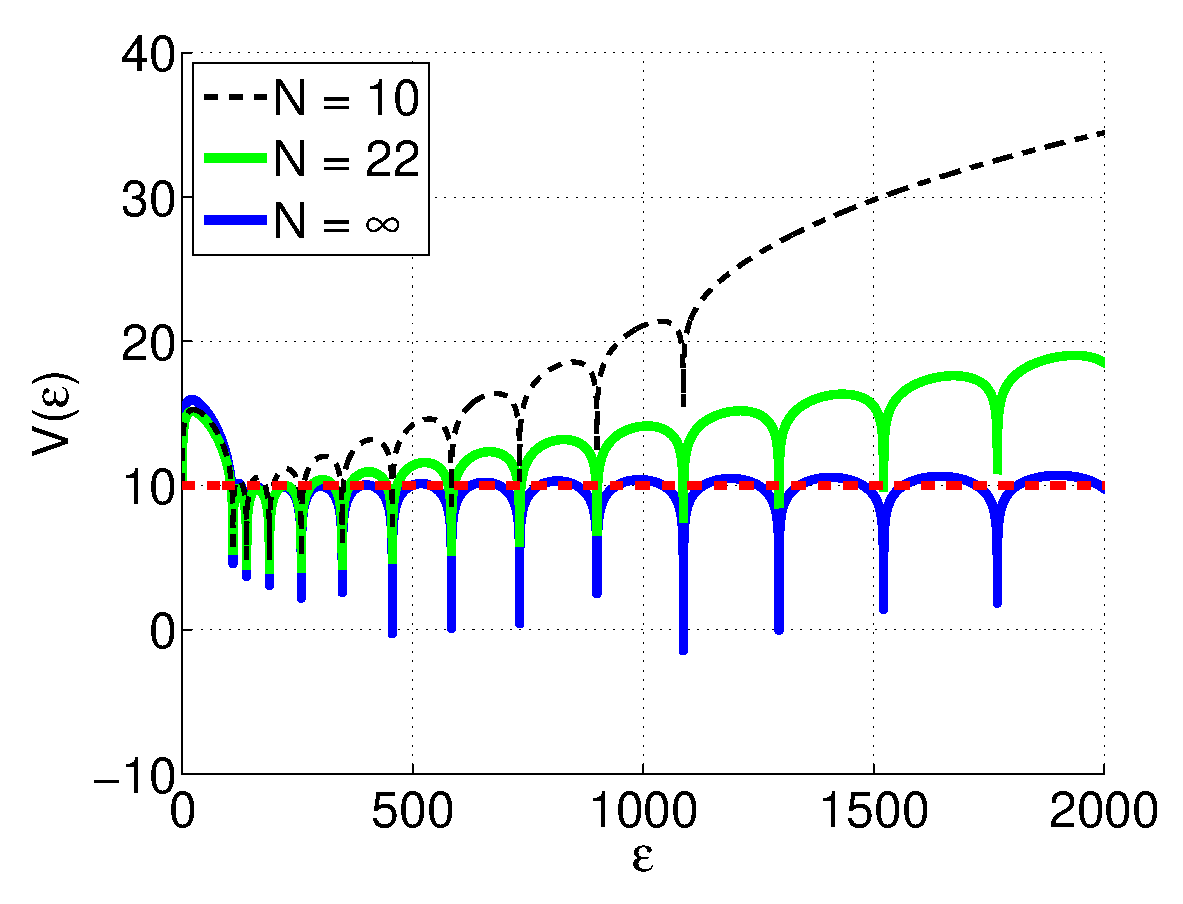
\includegraphics[height=5cm]{/Figs/gRing_ES_vs_cont}
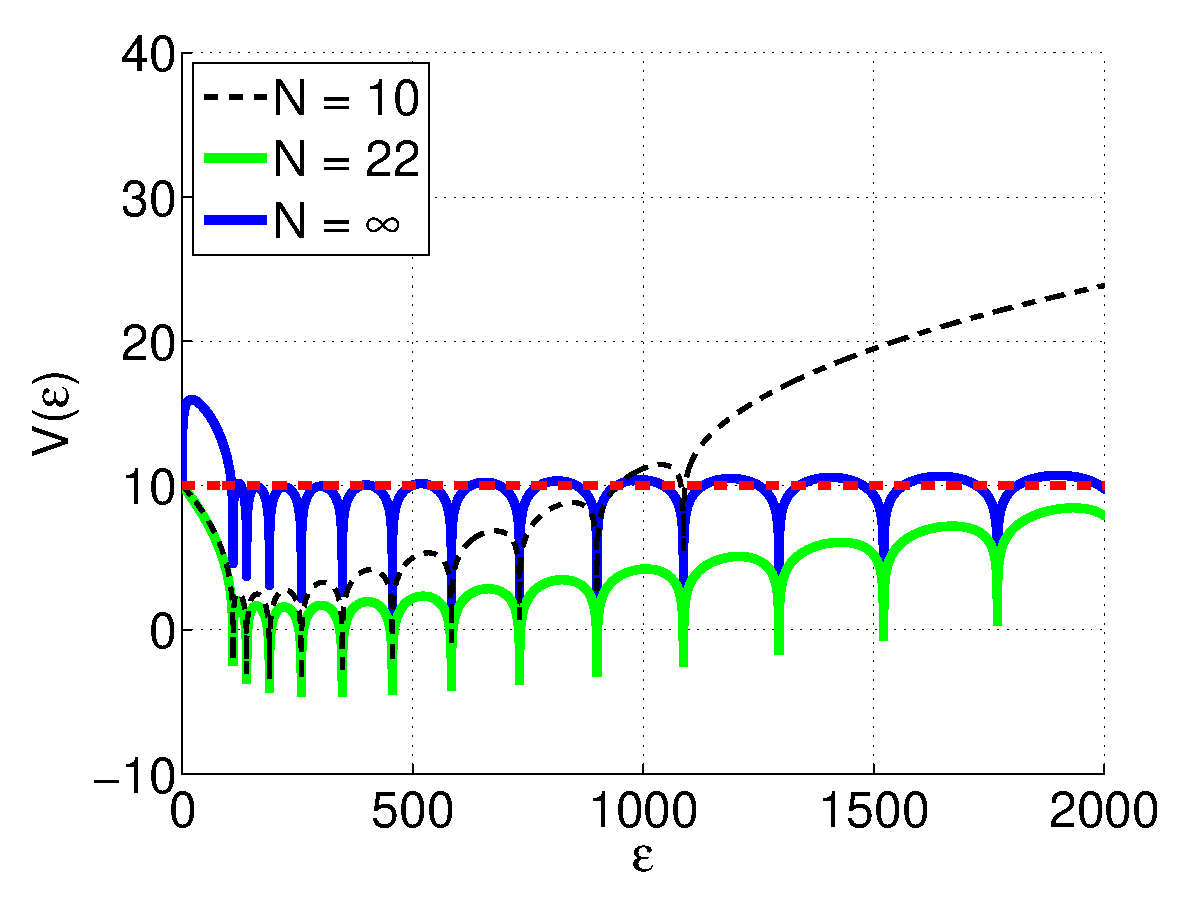
\includegraphics[height=5cm]{/Figs/gRing_ES_vs_cont2}
\caption{The secular equation of a continuous ring (solid blue) reconstructed using the electrostatic picture (green and black lines).
On the left panel the charge at the origin is included, while on the right it is not. 
The dashed red horizontal line is $V(0)=\ln(2\cosh(S/2)-2)$.
The charge at the origin is essential to determine the low energy behavior 
(On the left panel there is good agreement of the blue and green lines along the first few oscillations) , 
while the linear trend that appears in the electrostatic reconstruction is due to finite size truncation (as the number of charges is increased, the slope becomes smaller). 
For this figure, ${L=1, \ G=10^{-3}, \ s=20}$.}
\label{figReconstruction}
\end{figure}
%
%
%\subsection{Ground state of associated hermitian problem, $\epsilon_1$}
%\label{A6_1}
%If $S=0$ , then $\epsilon_k = \lambda_k$, so when $S$ is small we expect some correction.
%Thus, we expand \Eq{e1021} around $q_{\epsilon} = iS/2$ which corresponds to $\lambda = 0$, expand in powers of $S$ and solve for $q_{\epsilon_0}$ to obtain 
%%
%\beq
%q_{\epsilon_0}^2 = \frac{S^2}{4}\frac{1}{G-1}
%\eeq
%%
%and from \Eq{e1020}
%%
%\beq
%\epsilon_1= \frac{S^2}{4}\frac{G}{G-1}
%\eeq
%%
%\subsection{The spectrum}
%
%%
%To characterize the spectrum vs. $s$,  it is good to keep in mind two limiting cases.
%When $g=1$, we have a clean ring, and all eigenvalues are complex and they form a gapless continuum.
%When $g=0$, we have a chain, where all the eigenvalues are real. In this case there is a gapped continuum that begins at $\Gamma = s^2/4$. Note that the secular equation 
%derived earlier on is not valid for $g=0$.
%
%For finite $g$, the spectrum is gapped, however a "bubble" of complex eigenvalues can appear in the continuum. We obtain an analytical expression for the gap
%when the spectrum is real and prove that the gap is finite even when there are complex eigenvalues in the spectrum.
%
%Let us assume that $\lambda$ is real. 
%For given $S$, the left hand side of the secular equation \Eq{e1081} is oscilliatory, provided $\lambda > S^2/4$, otherwise, the trigonometric functions become hyperbolic.
%The oscillations are within an envelope function $\kappa(\lambda)$,
%%
%\beq
%\kappa(\lambda) = \sqrt{1+ \frac{1}{g^2}\frac{\lambda^2 }{4\lambda-S^2}}
%\eeq
%%
%There are real solutlons to the secular equation as long as the envelope function satisfies
%\beq
%\kappa(\lambda) > \cosh\left( \frac{ S}{2}\right)
%\eeq
%%
%which leads to the expression for the gap, provided that the spectrum is entirely real (\Fig{lambda_star}),
%%
%\be{1017}
%\text{Re}[\lambda] \geq {2g^2 \sinh^2(S/2)} \left[ 1 + \sqrt{1- \frac{S^2}{4g^2 \sinh^2(S/2)}}\right] \ \ =  \ \ \Delta(s)
%\eeq
%%
%
%\begin{figure}[h]
%\includegraphics[height=7cm]{real_lambda_contour.eps}
%\caption{The real part of the eigenvalues for an $L=100, \ D=1$ ring with a single diffusion barrier with 
%$g=10^3$ plotted vs. the affinity $s$. 
%The dashed black line is  \Eq{e1017}, which is the value of the gap and also indicates where the eigenvalues become complex.
%Notice that at the bottom of the band there is an eigenvalue that is always real.
%This plot was generated by producing a contour plot of \Eq{e1018} for real $\lambda$'s, it shows only real eigenvalues.
%}
%\label{lambda_star}
%\end{figure}
%
%When $S$ increases such that  $\cosh(S/2)>\kappa(\lambda)$, a complex "bubble" of eigenvalues appears.
%The bubble structure is due to the fact that the envelope function $\kappa(\lambda)$ has a global minimum at 
%$\lambda_{\min}=S^2/2$, so for  $\lambda > \lambda_{\min}$ the envelope function grows monotonically and will eventually intersect with $\cosh(S/2)$.
%This scenario is illustrated in \Fig{fig_f}.
%%
%The minimum value of the envelope function is
%%
%\beq
%  \kappa_{\text{min}} =\sqrt{ 1+\left(\frac{S}{2g}\right)^2}
%\eeq
%%
%The critical value $S_g$ such that for $S>S_g$ there are complex
%eigenvalues in the spectrum is determined by the transcendental equation (\Eq{e51})
%%
%\beq
% 1+\left(\frac{S}{2g}\right)^2 \ =  \ \cosh^2\left( \frac{S}{2} \right)
%\eeq
%%
%%
%%
%\begin{figure}[h]
%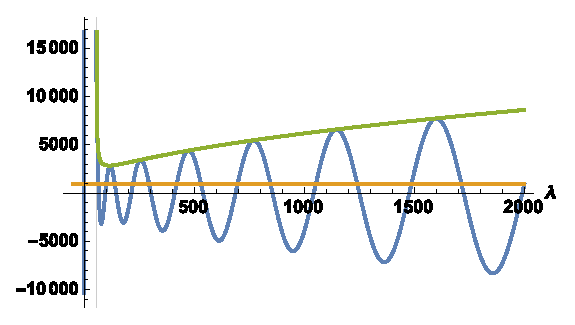
\includegraphics[width=7cm]{gRing3.eps}
%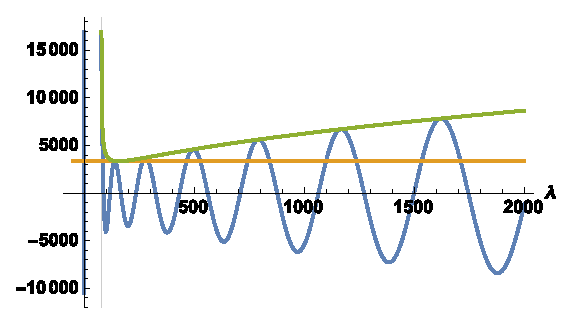
\includegraphics[width=7cm]{gRing2.eps}
%
%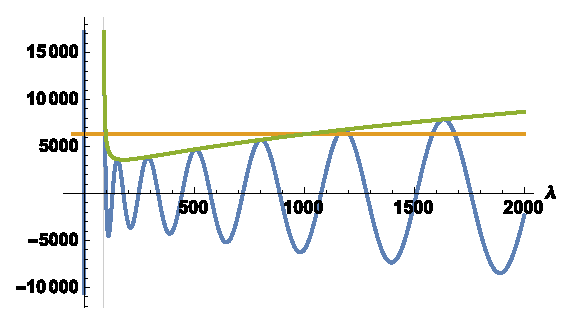
\includegraphics[width=7cm]{gRing1.eps} 
%
%\ \ \ \  \ \ \includegraphics[width=6cm]{gRing1Diagram}
%%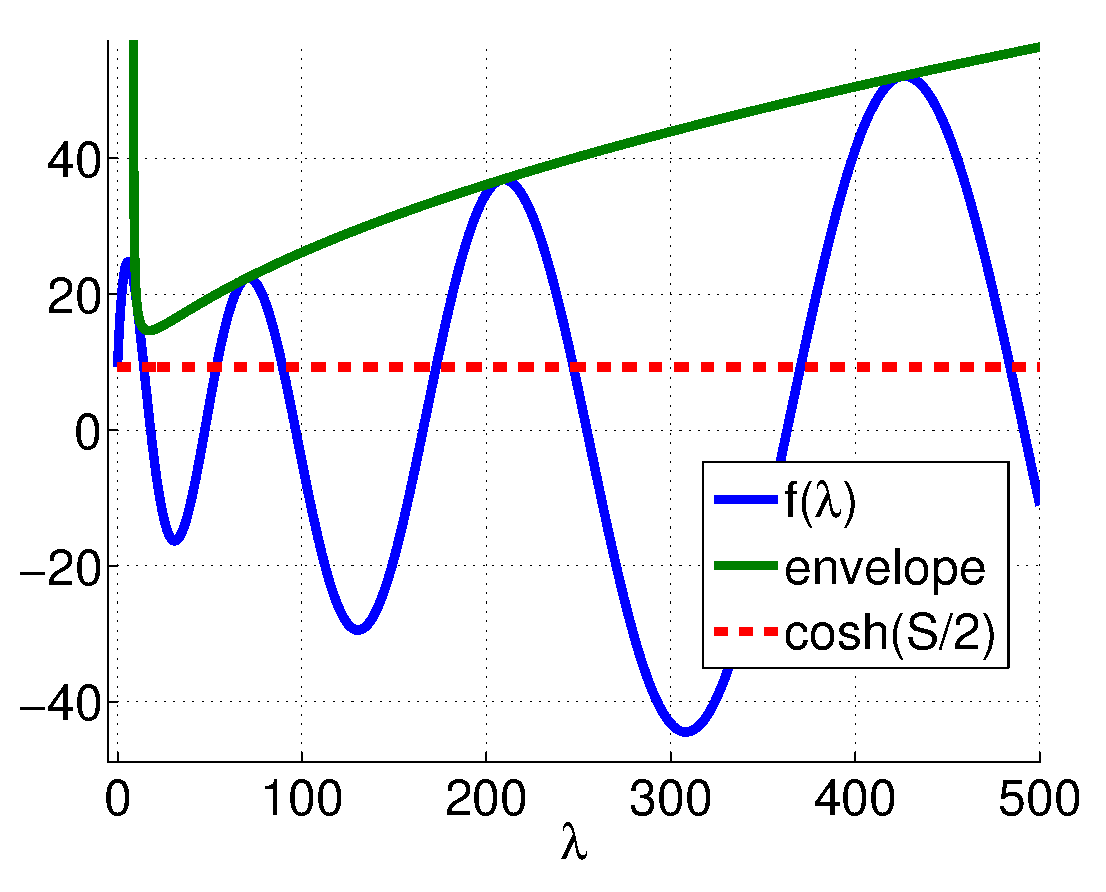
\includegraphics[height=4cm]{f_sg_m.eps}
%%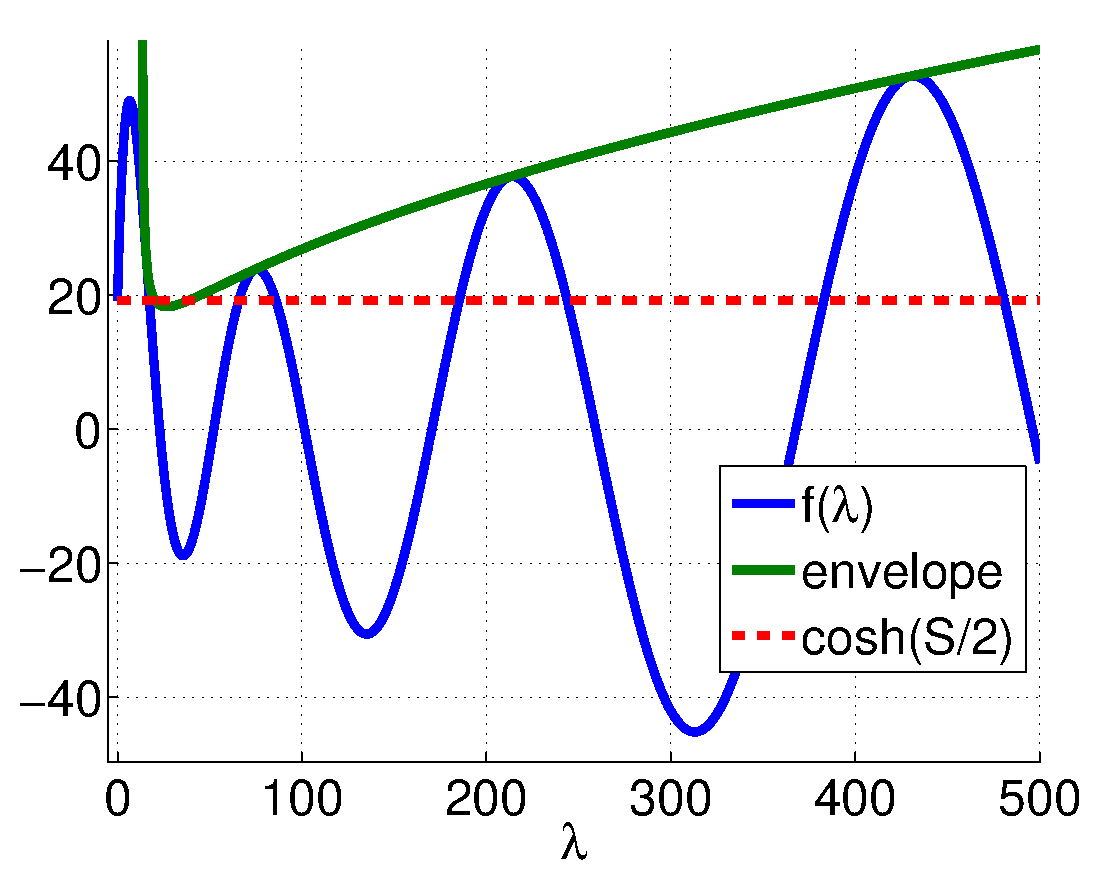
\includegraphics[height=4cm]{f_sg.eps}
%%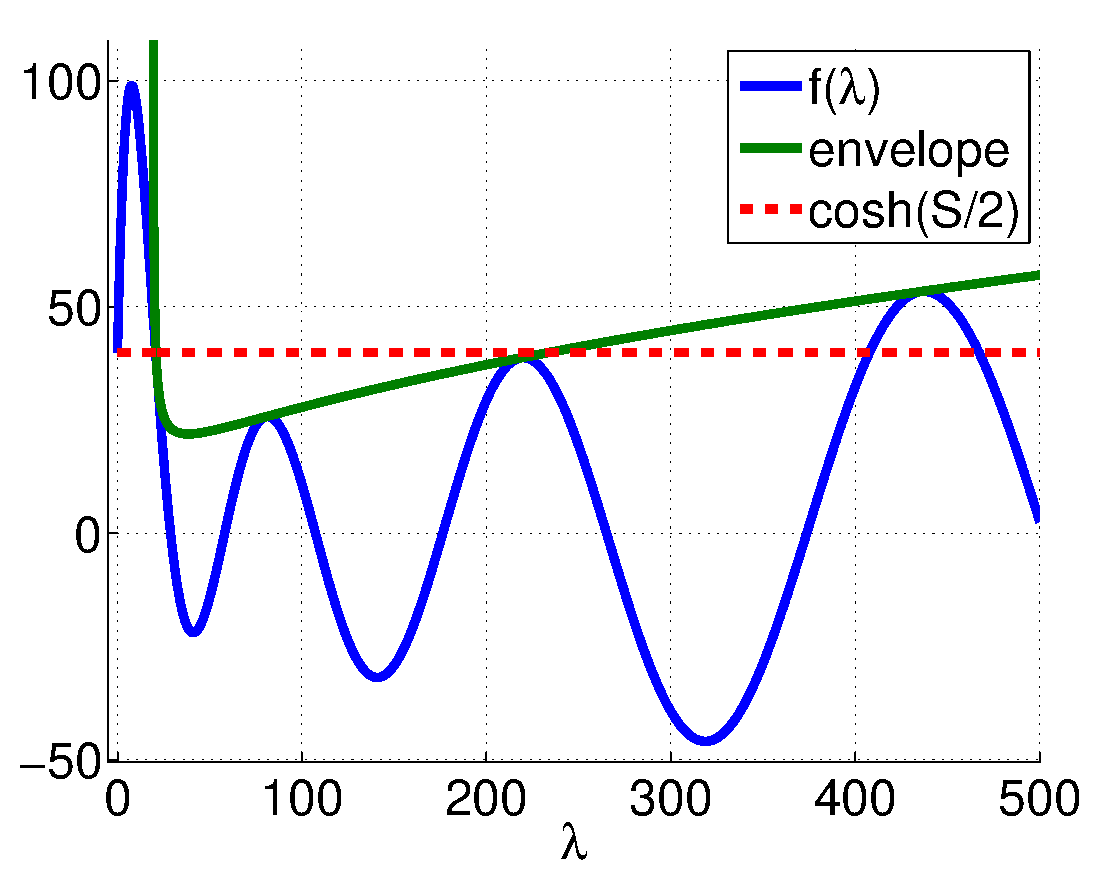
\includegraphics[height=4cm]{f_sg_p.eps}
%\caption{
%The secular equation $f(\lambda)=\cosh(S/2)$ for $g=1/380$, so $S_g=17.6$.
%Top row:  (left)  $S =15$ , all eigenvalues are real. 
%(right) $S = S_g$, marginal case.
%Middle row:l $S = 19$, the fully developed scenario, where the spectrum is initially real, then there is a "bubble" of complex eigenvalues and then the spectrum becomes real again. The high eigenvalues correspond to modes that decay very fast. Intuitively, since the high eigenvalues decay quickly, they cannot complete a trip around the ring before they decay, so they must be real. 
%The blue line is the oscillating part of the secular equation. The green line is the envelop function and 
%the horizontal orange line is $\cosh(S/2)$.
%In the bottom row we draw a schematic diagram of the spectrum in the complex plane of $\lambda$,
%corresponding to the fully developed scenario.}
%\label{fig_f}
%\end{figure}
%
%%%%%%%%%%%%%%%%%%%%
%\subsection{Proof the gap is finite}
%
%To show that the gap remains finite even when there are complex eigenvalues, it is more convenient 
%to use the second form of the secular equation 
%where the wave vector is  $z=x+iy$.
% The eigenvalues can be expressed in the following form 
% %
% \beq
%\lambda = (x+iy)^2+\left(\frac{S}{2}\right)^2 = x^2-y^2 + \left(\frac{S}{2}\right)^2 +2ixy
%\eeq
%%
%There is a trivial eigenvalue at $x=0, \ y=S/2$. 
%To show that the gap is finite, 
%it is sufficient to show that for $x\neq 0$,  $y<{S}/{2}$.
%Inserting $z=x+iy$, the secular equation splits in to two equations (for real and imaginary parts).
%%
%The real part of equation \Eq{e19} is 
%%
%\beq
%& &\cos (x) \left[ \cosh (y) - \frac{y}{g} \sinh (y) \frac{x^2+y^2 - S^2/4}{2(x^2+y^2)} \right] +\\
%&+& \sin(x) \left[ gx \cosh(y)\frac{x^2+y^2 + S^2/4}{2(x^2+y^2)}   \right]
%= \cosh\left(\frac{S}{2}\right)
%\eeq
%%
%This equation has the form $A(x,y) \sin(x) + B(x,y) \cos(x) = \cosh(S/2)$.
%For finite $x=x_1$, $y_1$ is determined by the 
%condition that the envelope of the function intersects with $\cosh(S/2)$
%%
%\beq
%\sqrt{A^2+B^2} = \cosh(S/2)
%\eeq
%%
%To prove that $y_1 < S/2$ it is enough to show that for $y=S/2$ the envelope satisfies
%$\sqrt{A^2+B^2} > \cosh(S/2)$.
%Assume that $g\gg 1$ and $S \gg S_g$, in this case there is a large bubble of complex eigenvalues so the gap is complex. Also, we can approximate 
%$\cosh y \approx \sinh y \approx e^y$ 
%and 
%$\cosh(S/2)\approx e^{S/2}$.
%%
%In this limit the envelope is 
%%
%\beq
%& & \left. \frac{1}{2g} e^y \sqrt{x^2+y^2} \sqrt{1+ \frac{S^2(x^2-y^2+S^2)}{2(x^2+y^2)}} \right|_{y=S/2} = \\
% & &
%\frac{e^{S/2}}{2g}
%\sqrt{x^2+(S/2)^2}
%\sqrt{1+\frac{S^2(x^2+3(S/2)^2)}{2(x^2+(S/2)^2)}} \ \ > \ \ e^{S/2}
%\eeq
%%
%so the solution must be $y<S/2$.
%%

\section{ Ring with single field defect}
\label{A8}

The field defect of the discrete ring translates to a defect in the velocity field in the continuum limit. 
We define a region $|x|<a/2$ in which the velocity field is different.
For $|x|>a$ we have $u/D=s$ and for $|x|<a$ we have $u/D=s+\sigma$. Note that for there to be a transition
from real to complex $s$ and $\sigma$ must have opposite signs. 
The boundary conditions are that the wave function and the current be continuous everywhere. 
Applying the boundary conditions across the defect and taking the limit $a\to 0$ such that $a\sigma = \Sigma(\text{const})$ we obtain the matching matrix at each boundary of the defect
%
\beq
S=\left(
\begin{array}{cc}
 1 & 0 \\
 \sigma  & 1 \\
\end{array}
\right)
\eeq
%
where $S$ is at $x=a/2$ and $S^{-1}$ at $x=-a/2$.
The transfer matrix is along a distance $x$ is $UT(x)U^{-1}$
where
%
\beq
U = \left(
\begin{array}{cc}
 1 & 1 \\
i\tilde k_{\sigma}+\frac{i s}{2} & -i\tilde k_{\sigma}+\frac{i s}{2} \\
\end{array}
\right)
\eeq
and 
%
\beq
T = \left(
\begin{array}{cc}
 e^{i \left(\tilde k_{\sigma}-\frac{i s}{2}\right) x} & 0 \\
 0 & e^{i \left(-\tilde k_{\sigma}-\frac{i s}{2}\right) x} \\
\end{array}
\right)
\eeq
%
Note that inside the defect $s\to s+\sigma$ and $\tilde k\to \tilde k_{\sigma} =  \sqrt{\lambda/D-(s+\sigma)^2/4}$ 
while outside the defect $s\to s$ and $\tilde k\to \sqrt{\lambda/D - s^2/4}$.
The matching condition between two sides of the defect is obtained by propagating the wave 
between the edges of the defect and taking the limit $a\to 0 $ while keeping $a\sigma$ constant,
%
\beq
M =\lim_{a\to 0} S^{-1} U_{\sigma} T_{\sigma}(a) U_{\sigma}^{-1} S= 
\left(
\begin{array}{cc}
 e^{\Sigma } & 0 \\
 \left(-1+e^{\Sigma }\right) s & 1 \\
\end{array}
\right)
\eeq
%
The subscript $\sigma$ is to indicate that $\sigma \neq 0$/
For a ring the wave function must obey
%
\beq
\left.\left( \begin{array}{c}
\psi \\
\partial \psi
\end{array}
\right)\right|_{x=0}  \ \ = \ \ 
T(L/2) M T(L/2)
\left.\left( \begin{array}{c}
\psi \\
\partial \psi
\end{array}
\right)\right|_{x=0} 
 \eeq
 %
which is possible only if 
%
\beq
\left|  T(L/2) {M} T(L/2) -I \right| =0
\eeq
%
This is the secular equation, which takes the explicit form
%
\beq
\cos \left(\frac{1}{2} \sqrt{4 \lambda -S^2}\right)\cosh \left(\frac{\Sigma }{2}\right)  \ + \ \frac{\sin \left(\frac{1}{2} \sqrt{4 \lambda -S^2}\right)}{\sqrt{4 \lambda -S^2}}S \sinh \left(\frac{\Sigma }{2}\right) \
= \cosh\left(\frac{S+\Sigma}{2}\right)
\eeq
%
It is easy to verify that $\lambda=0$ is a solution as required.
The envelope function is 
%
\beq
A(\lambda) \ = \ \sqrt{ \cosh^2 \left(\frac{\Sigma }{2}\right) \ + \
\frac{S^2}{{4 \lambda -S^2}} \sinh^2 \left(\frac{\Sigma }{2}\right) }
\eeq
%
with $A(0) = \cosh\left((S+\Sigma)/2\right)$.
The envelope function is monotonically decreasing for $\lambda > S^2/4$ reaching an asymptotic value 
%
\beq
\lim_{\lambda \to \infty} A(\lambda) = \cosh \left(\frac{\Sigma }{2}\right)
\eeq
%
Note that the true envelope function does not really explode at $\lambda=S^2/4$, because $\sinh(x)/x \to 1$ as $x\to 0$.
The condition for complexity is that 
%
\beq
A(0) > A(\infty)
\eeq
%
So $S_c$ is defined by the equation 
%
\beq
 \cosh \left(\frac{S+\Sigma }{2}\right) =  \cosh \left(\frac{\Sigma }{2}\right)
\eeq
%
As defined in the text, the affinity is the mean of the stochastic field, $s=(S+\Sigma)/L$,
thus the equation has a solution at $sL = \Sigma$
%
\beq
s_c L = \sigma a \ \ \Rightarrow \ \ s_c = \frac{\sigma}{N}
\eeq
%
as in \Eq{e32} of the text.

%%%%%%%%%%%%%%%%%%%%%%%%%%%%%%%%%%%%%%%%%%%%%%%%%%%%%%%
\section{ Ring with white disorder (�French�) }
\label{A9}
In the continuum limit, 
the density of states and electrostatic potential can be obtained analytically
for a an open ($L\to \infty$) one dimensional diffusion problem 
with a stochastic force field that is gaussian white noise 
with variance $\text{Var}(\mathcal{E}) = \sigma_g^2/a^2$ \cite{odh3}. 
First we present the basic equations in the continuum limit and proceed to present a summary of the results here in our notations.


We begin with the Langevin equation
%
\beq
\frac{dx}{dt} = \frac{1}{\gamma} F\left[x(t)\right] + \eta(t)
\eeq
%
where the environment is represented by thermal white noise 
%
\beq
\overline{\eta(t)} &=& 0 \\ 
\overline{\eta(t)\eta(t')} &=& \frac{2kT}{\gamma} \delta(t-t')
\eeq
%
and in the absence of disorder, by the Einstein relation we have 
%
\beq
D_0 = \frac{kT}{\gamma}
\eeq
%
The random force is gaussian 
%
\beq
\langle F \rangle &=& F_0 \\ 
\langle F(x)F(x') \rangle - F_0^2 &=& \sigma_g^2 \delta(x-x')
\eeq
%
where the overline represents averaging over thermal histories per given realization of disorder
and brackets represent ensemble average over different realizations of disorder. 
The equation for the probability distributions corresponding to the Langevin equation is the Fokker-Planck equation
%
\beq
\frac{\partial P}{\partial t} = D_0 \frac{\partial^2 P}{\partial x^2} - \frac{1}{\gamma} \frac{\partial }{\partial x} \left[ F(x) P\right]
\eeq
%
The drift velocity is thus 
%
\beq
u = \frac{F}{\gamma}
\eeq
%
along with the diffusion coefficient $D_0$, we have that 
%
\beq
\frac{u}{D_0} \ = \ \frac{F}{kT} \ \equiv \ s
\eeq
%
and does not depend on $\gamma$. 
%
The Fokker Planck equation can be obtained by taking the limit $a\to 0$ of the rate equation \Eq{e1} with transition rates 
%
\beq
w_{n,n+1} &=& \frac{D_0}{a^2}\exp\left[-a\frac{F_{n+1}}{2kT}\right]\\
w_{n+1,n} &=& \frac{D_0}{a^2}\exp\left[a\frac{F_{n+1}}{2kT}\right]\\
\eeq
%
So, in our language this is like having $D_0 = \overline{w} a^2$.
The dimensionless energy is 
\beq
\tilde{\epsilon} \equiv 16\frac{D_0^3}{\sigma_g^4} \epsilon 
\eeq
%
So the integrated density of states is 
%
\be{931}
\mathcal{N}(\tilde{\epsilon} )   \ &=& \ \frac{\sigma_g^2 N}{2D_0^2\pi^2}\frac{1}{ M_{\mu}^2 (\sqrt{\tilde{\epsilon} })}
\eeq
%
Where $\mu$ for gaussian white noise is ${\mu=2s/ \sigma_g^2}$.
Note that in the limit $\epsilon\to \infty$ the free particle result is recovered
%
\beq
\mathcal{N}(\epsilon) = \frac{N}{\pi} \sqrt{\epsilon/D_0}
\eeq
%
The electrostatic potential is
%
\beq
 V(\tilde{\epsilon} ) \ = \ -\sqrt{\tilde{\epsilon} } \frac{M'_{\mu}(\sqrt{\tilde{\epsilon} })}{M_{\mu}(\sqrt{\tilde{\epsilon} })} \frac{\sigma_g^2}{4D_0^2}, \ \ \tilde{\epsilon}  \geq 0
\eeq
%
where
\beq
M_{\mu}(\tilde{\epsilon} ) &=& \sqrt{J(\tilde{\epsilon} )^2_{\mu} + Y(\tilde{\epsilon} )^2_{\mu}}
\eeq
%

and $J_{\mu}$ and $Y_{\mu}$ are Bessel functions of the first and second kind.
%
In the limit $\epsilon \to 0$ we have for $\mu>0$
%
\beq
V(\epsilon) &=& 
\left\{
\begin{array}{cc}
\mu \nearrow 1/2, \ &  \mu<1/2 \\
\mu \searrow 1/2, \ &  \mu>1/2 
\end{array}\right.
\eeq


\begin{figure}
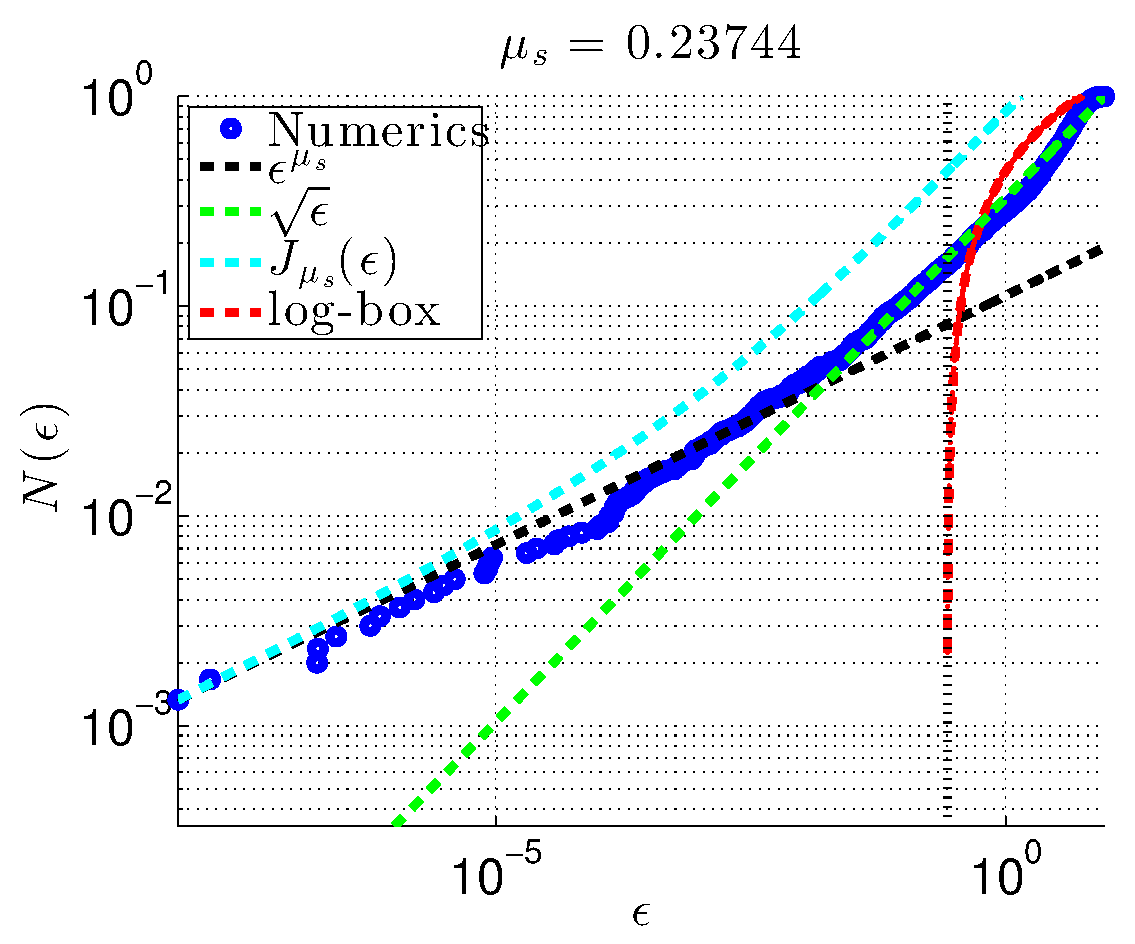
\includegraphics[height=4.5cm]{../Figs/N_E_1_french.eps}
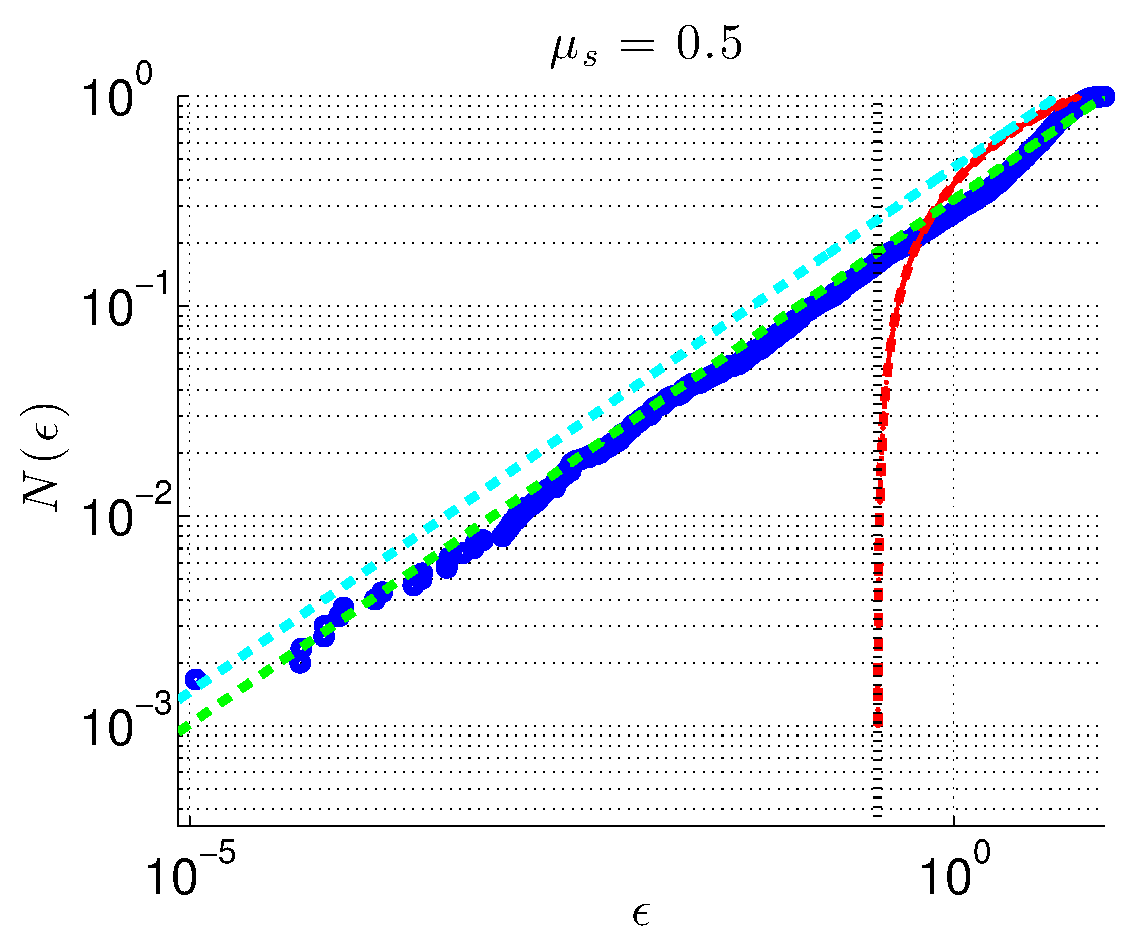
\includegraphics[height=4.5cm]{../Figs/N_E_2_french.eps}
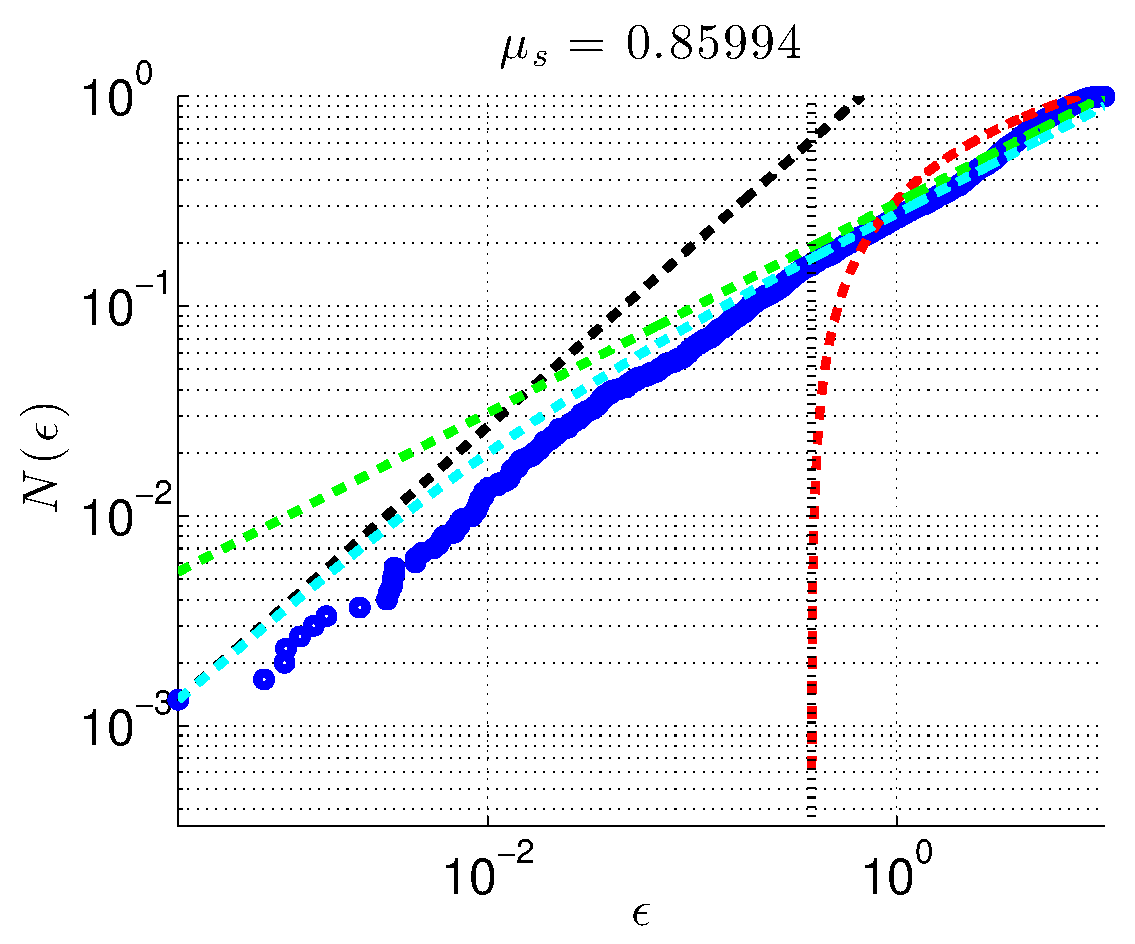
\includegraphics[height=4.5cm]{../Figs/N_E_3_french.eps}
\\ 
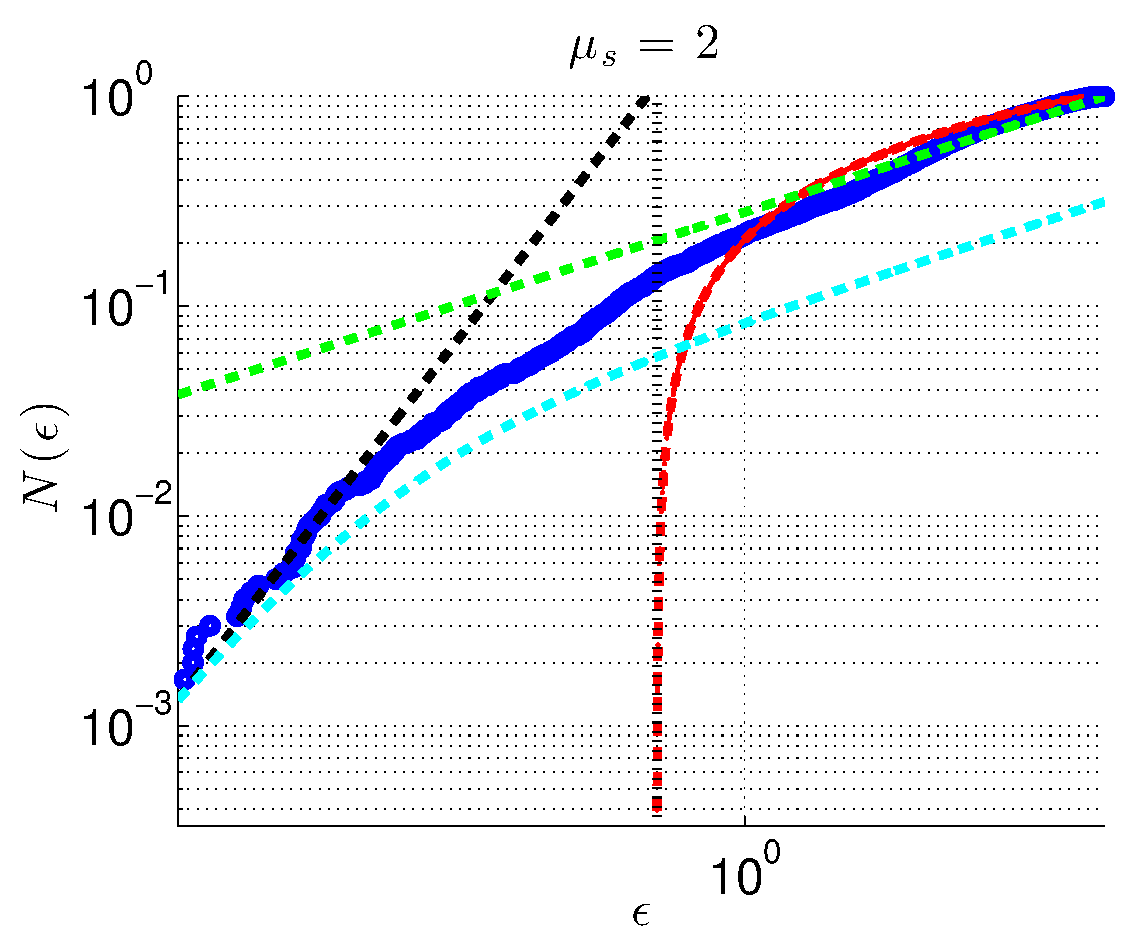
\includegraphics[height=4.5cm]{../Figs/N_E_4_french.eps}
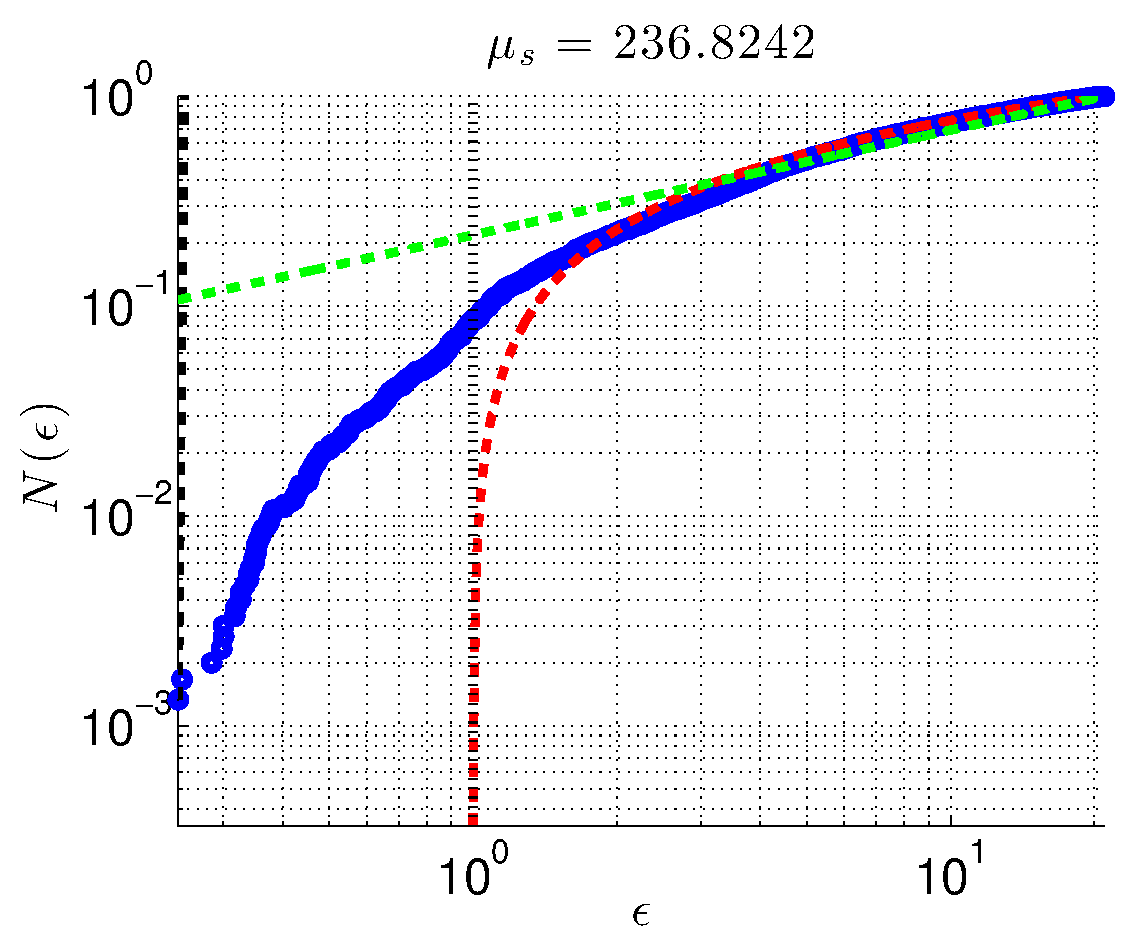
\includegraphics[height=4.5cm]{../Figs/N_E_5_french.eps}
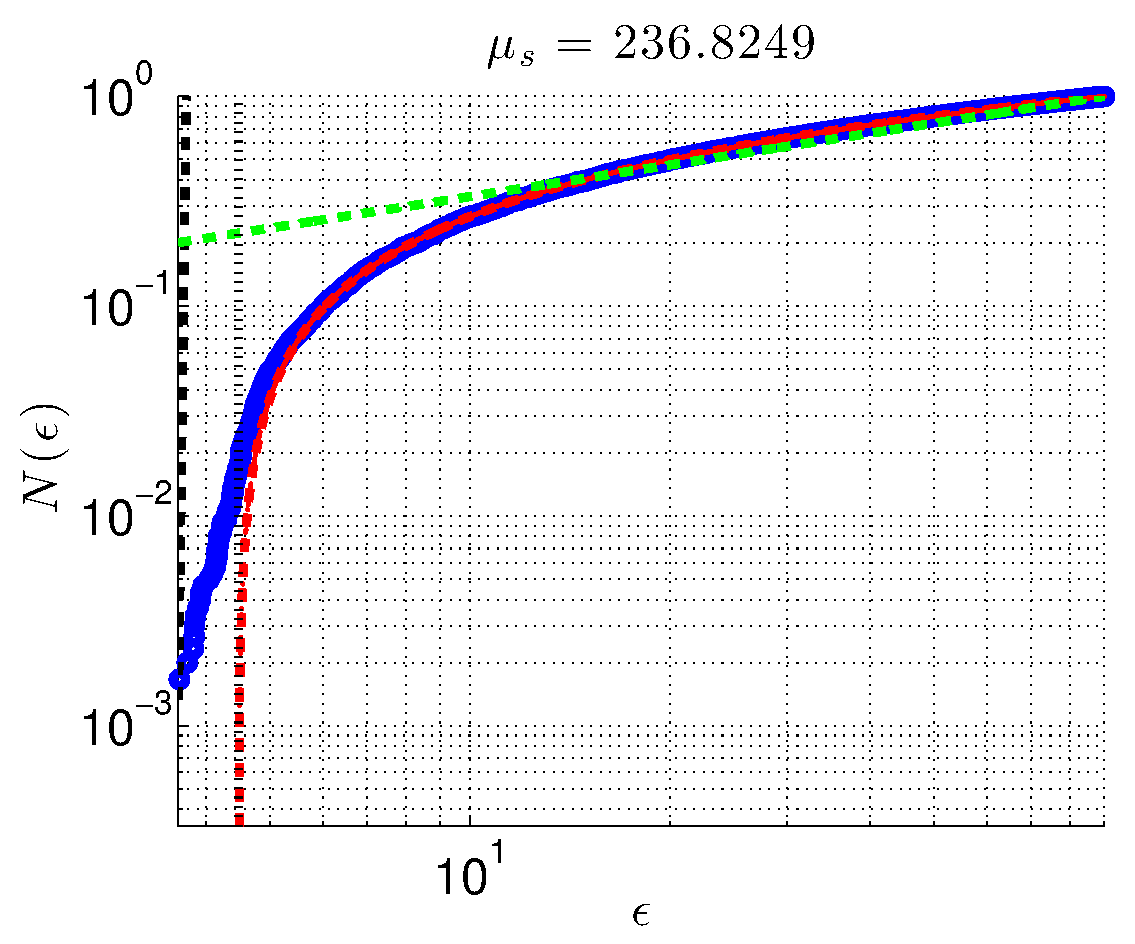
\includegraphics[height=4.5cm]{../Figs/N_E_6_french.eps}
\caption{The integrated density of states $N(\epsilon)$ for $N=3000, \ \sigma=3$ and $\alpha=\infty$. 
The dotted vertical line is $\epsilon_0=e^{(s-\sigma)/2}$.}
\end{figure}

\section{ Step by step electrostatics}
\label{A10}

The building blocks of the analysis are an isolated state, or point charge
and a continuum \Fig{stepByStep}. 
From these blocks we can construct any relevant 2D electrostatic potential.

{\bf Point charge.}  The potential of a single charge is simply 
%
\beq
V_{\text{charge}}(R) = \ln |R-\epsilon_1|
\eeq
%

{\bf Uniform charge.}
For a uniform charge distribution on the interval $x\in [a,b]$, the potential is given by the integral 
%
\beq
V(R) &=& \frac{1}{b-a}\int_a^b \ln |R-x| dx = \\
&=& \frac{1}{b-a}\left[(R-a)\ln|R-a| - (R-b)\ln |R-b| +a-b\right]
\eeq
%
which has a minimum at $R=(a+b)/2$ and resembles a "soft well" potential.

{\bf Continuum (clean ring).} 

For a continuum, or clean ring we show that the density is higher at the edges, leading to a "flat floor" potential.

The associated hermitian spectrum of a clean lattice ring is obtained by appropriately setting $s=0$ in \Eq{e12}
%
\beq
\epsilon_n = 2w\left[ \cosh \left(\frac{s}{2}\right) - \cos\left(\frac{2\pi}{N}n\right) \right]
\eeq
%
which can be inverted to obtain the integrated density of states
%
\beq
\mathcal{N}(\epsilon) \ = \ \frac{N}{2\pi }\arccos \left[  \cosh \left(\frac{s}{2}\right)  - \frac{\epsilon}{2w} \right]
\eeq
%
The density of states is 
%
\beq
\rho(\epsilon) &=& \frac{d\mathcal{N}}{d\epsilon} = 
\frac{N}{4\pi w}\left[ 1- \left(   \cosh \left(\frac{s}{2}\right)  - \frac{\epsilon}{2w}\right)^2\right]^{-1/2} 
\eeq
%
from which we obtain
%
\beq
\rho(k) = \frac{N}{4\pi w}\left[ 1-\cos^2 (k)\right]^{-1/2} =  \frac{N}{4\pi w\sin(k) }
\eeq
%
The electrostatic potential formed by a charge distribution $\rho(\epsilon)$ is given by means of \Eq{e23}
%
\beq
V(R) = \int_a^b  \ln \left| \frac{\epsilon - R}{w}\right| \rho(\epsilon) d\epsilon = 
\frac{N}{2\pi} \int_0^{2\pi} \ln \left| 2\cosh\left(\frac{s}{2}\right) - 2\cos(k) - R\right| dk 
\eeq
%
where $[a,b] = 2w[\cosh(s/2) \pm 1]$. 
%The potential is an oscillating function but the peaks form an envelope
%function that has the values 
%%
%\be{1070}
%V_{\text{continuum}}(R) \  \approx  \ \frac{N\ln(2)}{\pi} \ + \
%\left\{\begin{array}{cc}
%  \frac{N}{2\pi}\sqrt{|R-a|} &, \ \ R<a \\
%& \\
%0 &, \ \  R>a
% \end{array}
% \right.
% \eeq
%%

\begin{figure}[h]
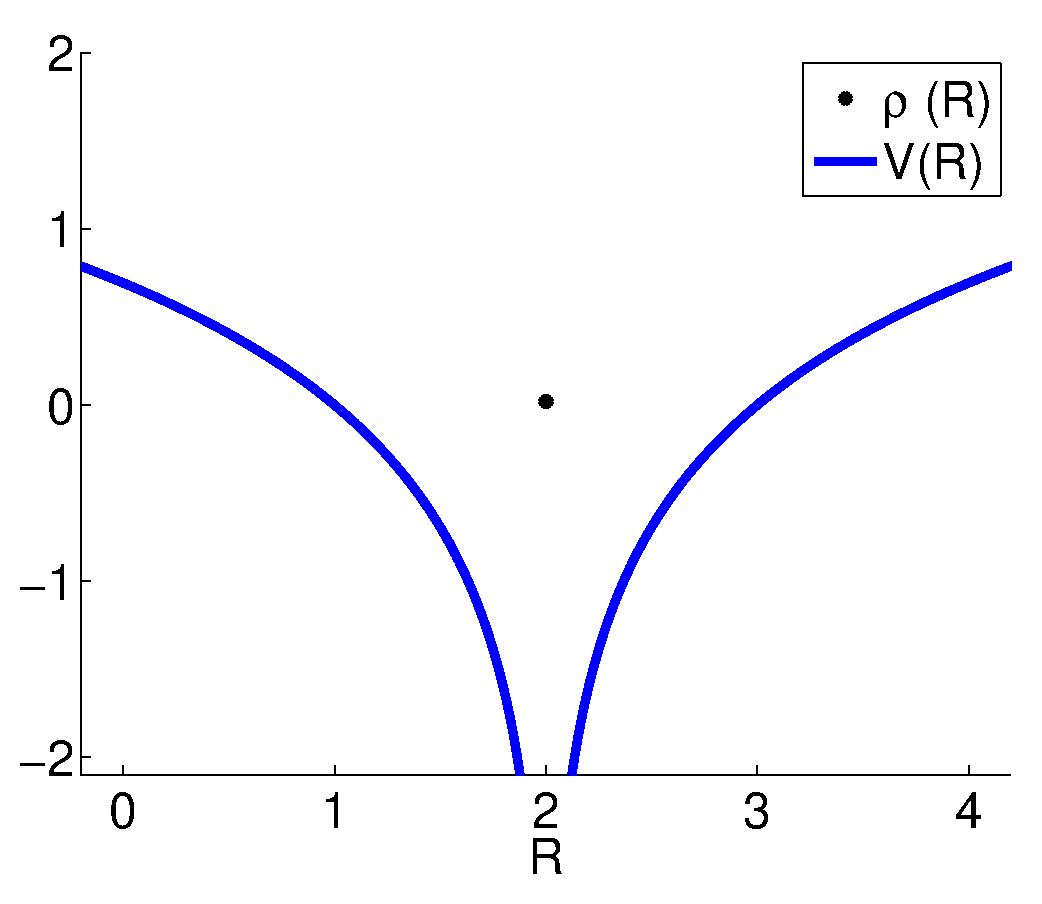
\includegraphics[height=4cm]{/Figs/V_R_stepbystep_point}
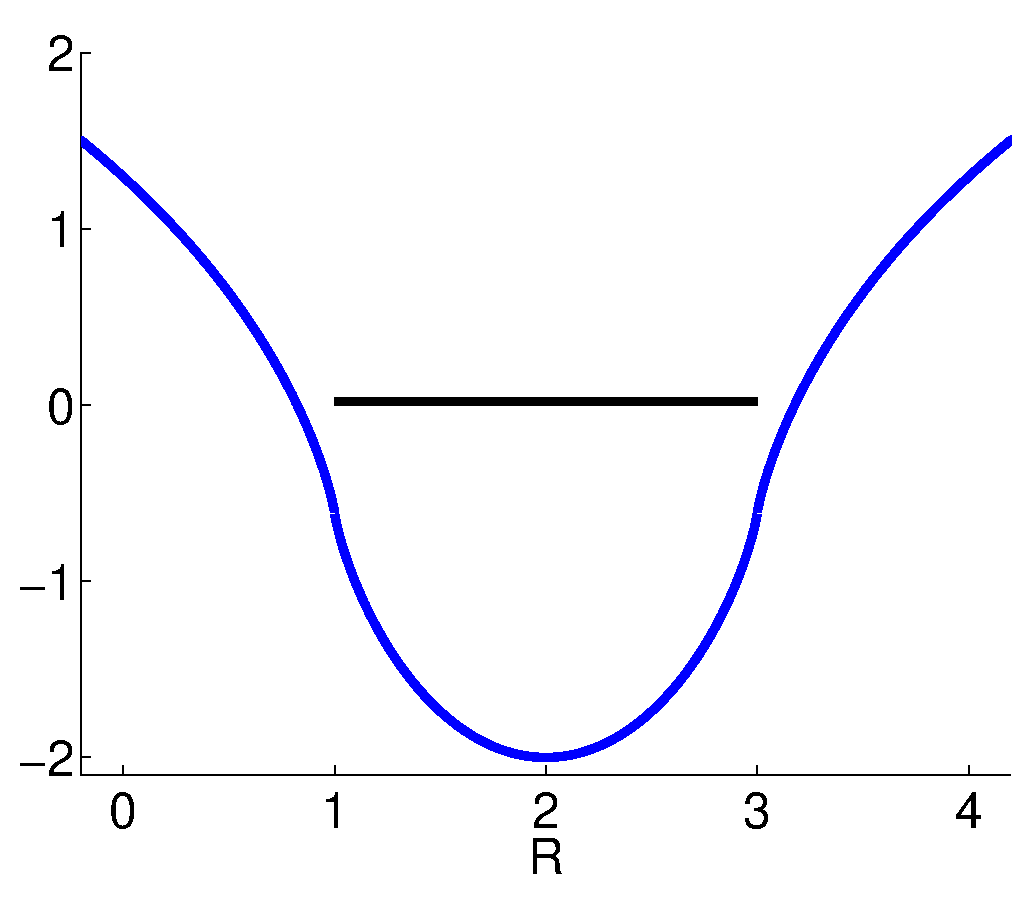
\includegraphics[height=4cm]{/Figs/V_R_stepbystep_uniform}
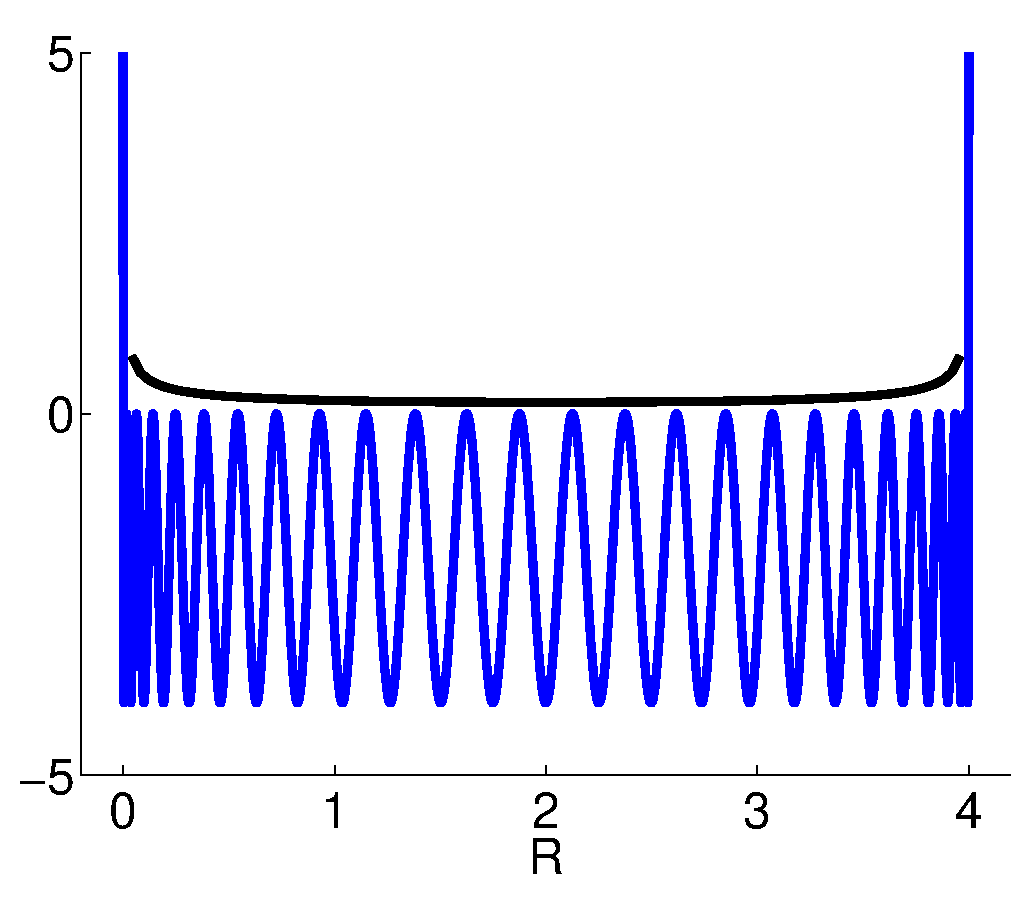
\includegraphics[height=4cm]{/Figs/V_R_stepbystep_continuum}
\caption{The building blocks of the electrostatic picture. 
A point charge at $R=2$ (left) generates a logarithmic potential, a uniform charge distribution on the interval $[1,3]$ (middle) generates a soft well
and a clean ring with $s=0$ (right) generates a flat floor (any $s\neq 0$ just shifts the charge density to the right). 
The potential is the blue line and the charge density is drawn in black.
For the clean ring we plot the spectral determinant instead of the potential, in order to show that the floor is really at zero.
}
%
%The electrostatic potential of a clean ring, \Eq{e1070} (blue). 
%The potential is flat (dashed red line) where the density of states  (black curve) is not zero
%and diverges as $\sqrt{|R|}$ elsewhere (green line)}
\label{stepByStep}
\end{figure}

\section{The NESS formula}
\label{Ap12}
%
The left eigenvector of ${\bm W}$ with eigenvalue $\lambda_0=0$ is 
the non-equilibrium steady state, and is given by the following formula (The derivation appears in \cite{nef}, however there is a typo in the last line and the notation is somewhat confusing. The correct version is given here.)
We have shown that the master equation can be rewritten in the form 
%
\beq
I = \left( \overleftarrow{G}_n {-} \overrightarrow{G}_n  \right)p_{n},  
\eeq
%
where $\overrightarrow{G}_n$ is determined by "cutting" the ring at $n$
equation 17 of \cite{nef} becomes 
%
\beq
\overrightarrow{G}_n \  \ &=& \ \ \left[ \sum_{r=0}^{N-1} \frac{1}{w_{\overrightarrow{n+r+1}}} 
\,\exp\left(-\sum_{x=n+1}^{n{+}r} \mathcal{E}_x \right) \right]^{-1} 
\eeq
%
It is easily seen that ${\overleftarrow{G}_n = \exp(-S) \, \overrightarrow{G}_n}$
and by definition, 
%
\beq
p_n = I/( \overleftarrow{G}_n - \overrightarrow{G}_n)
\eeq
%
so we have
%
\beq
p_n &\  \propto \ & 
\sum_{r=0}^{N-1} \frac{1}{w_{\overrightarrow{n+1+r}}} \exp \left[  - \sum_{x=n+1}^{n+r}  \mathcal{E}_x\right] = \sum_{r=0}^{N-1} \frac{1}{w_{\overrightarrow{n+1+r}}} e^{  U(n+r)-U(n)-s\cdot r} = \\
& \ = \ & \left (\sum_{r=0}^{N-1} \frac{1}{w_{\overrightarrow{n+1+r}}} e^{  U(n+r)-s\cdot r} \right)
e^{-U(n)} \ \equiv \ \left( \frac{1}{w_{\overrightarrow{n}}}\right)_s e^{-\left(U(n)-U_s(n)\right)}
\eeq
%
where the potential $U(X)$ is defined via
%
\beq
\sum_{x'}^{x''} \mathcal{E}_x \ = \ U(x'){-}U(x'') + s\cdot(x''{-}x')
\eeq  

\end{document}
%%%%%%%%%%%%%%%%%%%%%%%%%%%%%%%%%%%%%%%%%%%%%%%%%%%%%%%%%%%%%%%%%%%%%%%%%%
%%%%%%%%%%%%%%%%%%%%%%%%%%%%%%%%%%%%%%%%%%%%%%%%%%%%%%%%%%%%%%%%%%%%%%%%%%


